\documentclass[11pt,a4paper,oneside]{article}
\usepackage[utf8]{inputenc}
\usepackage{amsmath}
\usepackage{amsfonts}
\usepackage{amssymb}
\usepackage{url}
\usepackage{graphicx}
\usepackage{geometry}
 \geometry{
 a4paper,
 total={170mm,257mm},
 left=20mm,
 top=20mm,
 }
 
\setlength{\parskip}{1em} 
 
\author{John Walmsley, Gary R.~Mirams}
\title{Predicting simulation-experiment discrepancy in cell-specific cardiac electrophysiology models}

\newcommand{\norm}[1]{\left\lVert#1\right\rVert}

\begin{document}

\maketitle

\section{Introduction}

Acquired Long QT syndrome (aLQTS) leading to potentially lethal torsade de pointes arrhythmias has been a rare complication of pharmaceutical treatment with serious consequences for patients, clinicians, regulators and pharmaceutical companies\cite{Roden2004}. At present, screening for pro-arrhythmic side effects is performed using the Thorough QT study. This study is extremely sensitive but highly aspecific, leading to the likely removal of many safe compounds at early stages of drug development, increasing costs of development and reducing the number of beneficial compounds that can be taken forwards through the drug development pipeline.

In response to the present unsatisfactory situation, the United States Food \& Drug Administration (FDA) has launched the Comprehensive \textit{in vitro} Pharmaceutical Assay (CiPA) project in collaboration with academic researchers, safety pharmacologists and key regulatory bodies\footnote{\url{http://cipaproject.org/}}. CiPA aims to improve or replace existing screening methods with assays that use computational cardiac cell models representing human cardiac electrophysiology and/or human induced pluripotent stem cell-derived cardiomyocytes\cite{Colatsky2016}. A particular focus of the CiPA project is characterisation of the activation and drug binding kinetics of the hERG channel, which carries the crucial rapidly activating delayed rectifier potassium current (I$_{\text{Kr}}$). I$_{\text{Kr}}$ is a key component of cardiac repolarization and is commonly implicated in aLQTS.

As part of the CiPA initiative, Beattie \textit{et al} recently published a novel method for fitting hERG channel kinetics on a cell-specific basis that uses a novel `sine wave' voltage clamp protocol as training data to parameterise a simple model of the hERG channel\cite{Beattie2018}. This model has four `states' and is analogous to the Hodgkin-Huxley potassium current model. The resultant fits produced an excellent qualitative fit to prediction data based on a combination of action potential voltage waveforms. The resultant parameterized model outperformed existing characterisations of IKr extant in the modelling literature with a range of different model structures. Consequently, this new method for characterizing hERG channel kinetics is highly promising for the CiPA project, as it offers a way to characterise recorded kinetics from high-throughput data, while requiring a fraction of the data (and hence recording time) required by long traditional step protocols which can require multiple cells to parameterise adequately, which may be prohibitive for applications which also require characterisation of channel kinetics in presence of pharmaceutical agents.

To advance this promising model parameterisation approach further for application in pharmaceutical development pipelines, several key issues still need to be addressed. Namely 1) can we quantify our certainty in the predictions of the parameterised model, and 2) does the discrepancy between the parameterised model and the experimental data arise due to an inadequate model structure, or an inadequate parameterisation of the model? This report descibes attempts to address these questions using regression methods.

\section{Models of the hERG Channel} \label{Sec_ModelsOfHerg}

In this study, we will focus on two formulations of models for hERG. The first is a standard Hodgkin-Huxley model written in a Markov formulation, as used by Beattie et al\cite{Beattie2018},
\begin{align}
		\frac{d[C]}{dt}&= -(k_1+k_3)[C] + k_2 [O] + k_4[IC],\\ \label{Eq_dCdt}
		\frac{d[O]}{dt}&= -(k_2 + k_3 )[O] + k_1 [C] + k_4 [I],
		, \\
		\frac{d[I]}{dt}&= -(k_2 + k_4 )[I] + k_3 [O] + k_1 [IC],\\
		 [IC] &= 1 - ([C] + [O] + [I]),
\end{align}

where $ \left[ C \right] $ is the closed, $ \left[O \right]$ the open, $\left[ I \right]$ the inactive and $\left[ IC \right]$ the inactive and closed state probability. The rate constants are given by,
\begin{align}
k_1 & = P_0 \exp(P_1 V),\\ 
k_2 & = P_2 \exp( - P_3 V),\\ 
k_3 & = P_4 \exp(P_5 V),\\
k_4 & = P_6 \exp(- P_7 V).
\end{align}
The current arising from this model is given by,
\begin{align}
I & = G [O] (V-V_R), \label{Eq_I_hh}
\end{align}
where $G$ is the conductance of the channel, $V$ is the membrane potential and $V_R$ is the Nernst potential for potassium ions, a quantitiy that can be calculated from a patch clamp experiment. For the rest of this report we will label these results using $y_1 = [IC]$, $y_2=[I]$, $y_3 = [O]$ and $y_4 = [C]$ to be consistent with the Matlab code. $k_{ij}$ will denote the transition from state $i$ to state $j$.

Equivalently, the above model can be reformulated as follows,
\begin{align}
\frac{dm}{dt} & = \frac{m_{\infty} - m}{\tau_m},\\ \label{Eq_dmdt}
\frac{dh}{dt} & = \frac{h_{\infty} - h}{\tau_h},
\end{align}
where, 
\begin{align}
m_{\infty} & = \frac{k_1}{k_1+k_2},\\
\tau_{m} & = \frac{1}{k_1+k_2},\\
h_{\infty} & = \frac{k_3}{k_3+k_4},\\
\tau_{h} & = \frac{1}{k_3+k_4},
\end{align}
and the current is given by
\begin{align}
I & = G m h(V-V_R). \label{Eq_mh}
\end{align}
An advantage of this formulation is that it allows for more complex forms of the model to be generated quickly using the same equations for $m$ and $h$, for example,
\begin{align}
I & = G m^2 h(V-V_R), \label{Eq_m2h} \\
I & = G m^3 h(V-V_R),\\
I & = G m^4 h(V-V_R),\\
I & = G m^2 h^2(V-V_R). \label{Eq_m2h2}
\end{align}
We will return to the latter form of equations in Section \ref{Sec_ModelDiscrepancy}.


\section{Definition of Discrepancy} \label{Sec_ModelsOfDiscrepancy}
\subsection{Simulation discrepancy}
"Model discrepancy" can be defined in different ways. For the purposes of this project, we will be using two different definitions. The first (in line with the CIPA goals described above) is the discrepancy between the model and the target trace $I_{exp}$, which may be experimental data or some other simulated data. We can sub-divide this definition in terms of how we consider this discrepancy. The first method is very simple:
\begin{align}
	I_{exp} = G O ( V - V_E ) + d\\
	d = I_{exp} - G O ( V - V_E ) \label{discrepancy_d}
\end{align}
This is the difference between model simulation and data, used in \cite{Beattie2018} in the least squares fitting procedure. The second definition is more natural from a physiological point of view, but less well behaved mathematically. Because the measured current is proportion to the open probability of the channel and the (known) voltage, we can also consider
\begin{align}
	I_{exp} = G ( O + d_o ) ( V - V_E )\\
	d_o = \frac{I_{exp} }{ G( V - V_E ) } - O \label{discrepancy_do}
\end{align}
Because of the singularity around the Nernst potential $V_E$, we need to remove these points from the trace - most traces spend relatively little time at these potentials (~-88mV). In this project, a 5mV window either side of the Nernst potential was discarded. These definitions of discrepancy are used in Sections \ref{SubSec_Lasso_Discrepancy} and \ref{SubSec_StepwiseLM_Discrepancy}. Plots of both forms of discrepancy for the sine wave and action potential protocols are shown in Fig.~\ref{Fig_Discrepancy}.

\begin{figure}[t]
\begin{center}
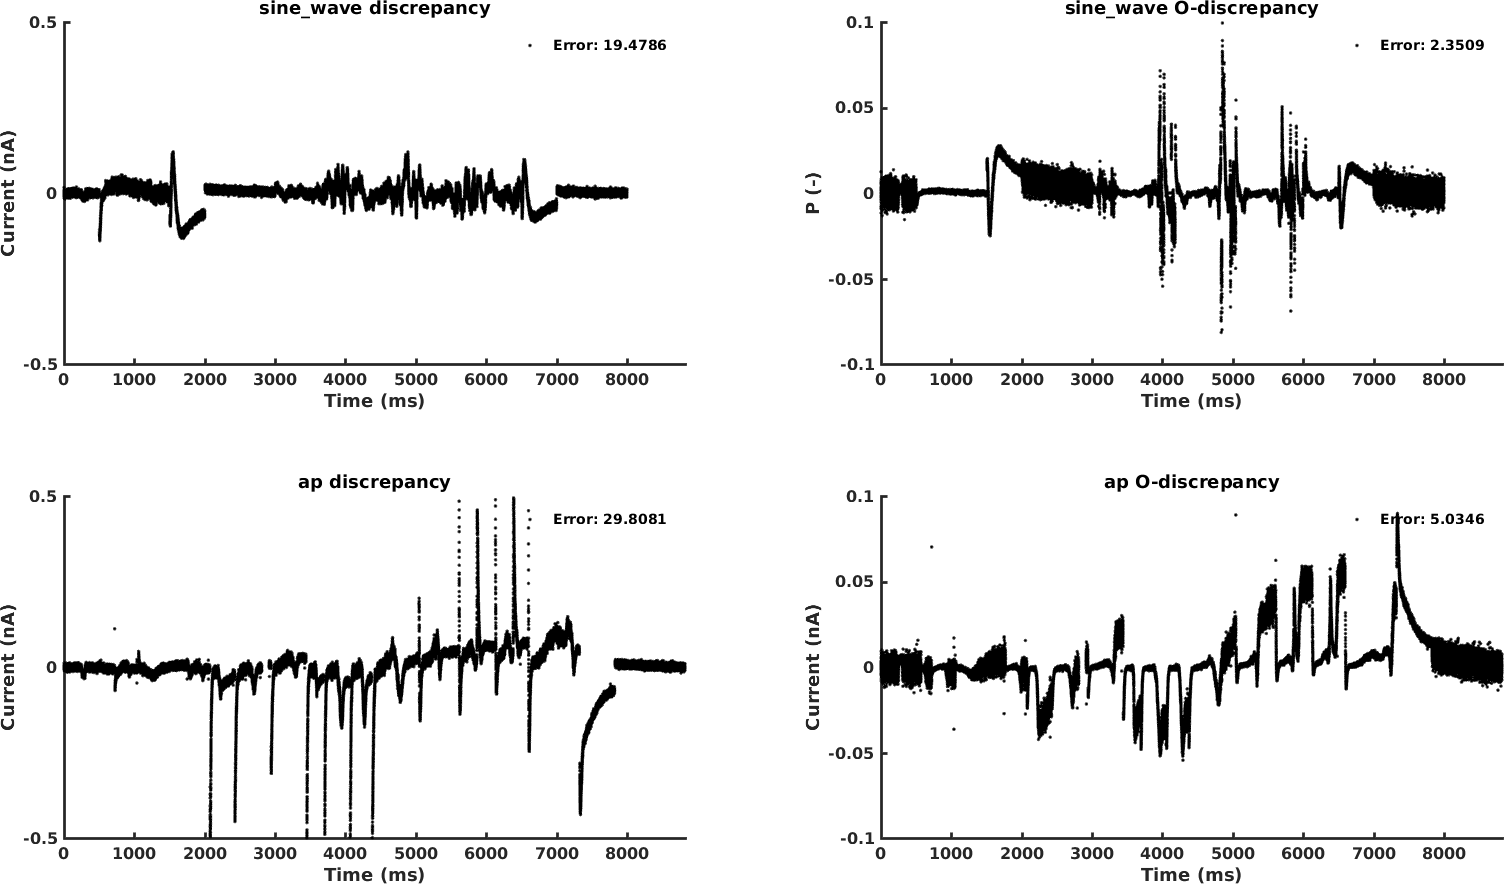
\includegraphics[scale=0.42]{Figures/PlotDiscrepancyVsDiscrepancyInOpen_sine_wave_ap.png}
\caption{\textbf{Discrepancies for the sine wave (top) and action potential (bottom) protocols.} The left hand column shows $d$ and the right hand column shows $d_o$. Capacitative spikes have been removed.}
\label{Fig_Discrepancy}
\end{center}
\end{figure}


\subsection{Structural discrepancy}
Both of the above definitions rely on a particular parameterisation of the model. However, it is also possible to consider the model discrepancy as being the difference between the model and reality. This concept is explained in more detail in \cite{Kennedy2002} and \cite{Strong2014} and refers to the structure of the model rather than its parameterisation.  This definition of model discrepancy refers to model structure, rather than model parameterization (which would change $d$ and $d_o$, above). In the context of hERG modelling, this could be a relatively simple difference, such as the number of closed states in a model or the form of the rate constants. Alternatively, it could be an entirely different feature not preserved in the model of interest - consider the difference between a molecular dynamics simulation of channel opening and a four state Markov model. In this project, we considered this form of discrepancy by fitting four models to the same data and then exploring how their evolution differed in time (Section \ref{Sec_ModelDiscrepancy}).

\section{Statistical Prediction of Discrepancy}

\subsection{Introduction}

Our goal was to predict simulation discrepancy when using fitted models for prediction. The goal would then be to quantify, based on the training data and the prediction simulation, where and by how much the prediction simulation would differ from the actual experimental trace recorded from that cell, for the prediction protocol. In this report, we use two methods, LASSO and the Matlab method Stepwise Linear Model.

\subsection{Input Variables}\label{SubSec_Predictors}

As an initial hypothesis, we proposed to use properties derivable from the model equations shown in Eqs.~\eqref{Eq_dCdt}-\eqref{Eq_I_hh}. These properties are
\begin{itemize}
\item Variables $y_1$, $y_2$, $y_3$, $y_4$.
\item Rates $K_{ij}$
\item Fluxes $y_i K_{ij}$
\item Current $I$
\item Voltage $V$
\item Voltage time derivative $\frac{dV}{dt}$
\item Time $t$
\item Parameter sensitivities $\frac{dy_i}{dp_j}$
\item Current sensitivity $\frac{dI}{dp_j} = G \frac{dy_3}{dp_j} (V-V_E) $
\end{itemize}

Parameter sensitivities are derived using the following equation \cite{}. Using $s_{ij} = \frac{dy_i}{dp_j}$,
\begin{align}
	\frac{\partial}{\partial p_j} ( \frac{dy_i}{dt} ) & = \frac{\partial}{\partial p_j} (f( y ) ) \\
	\frac{d}{dt}(\frac{\partial y_i}{\partial p_j})   & = \frac{\partial f}{ \partial y_i}\frac{\partial y_i}{ \partial p_j} + \frac{\partial f}{ \partial p_j} \\
	\frac{d s_{ij}}{dt} & = \frac{\partial f}{ \partial y_i} s_{ij} + \frac{\partial f}{ \partial p_j}
\end{align}
The CVODES libraries are used to integrate the parameter sensitivity equations alongside the ODEs in Eqns.~\eqref{Eq_dCdt}-\eqref{Eq_I_hh}.

Before performing any estimation, we check for linear dependence of each set of properties in turn, then check for linear dependence of all the properties that remain. The linear independence check is numerical and performed using the Mathworks File Exchange program getLinearDependent.m. Note that we did not include the derivatives of the variables ($\frac{dy_i}{dt}$) because they are linear combinations of the fluxes.

\subsection{Experimental Data}
For the purposes of this study we restricted ourselves to one cell from the study by \cite{}, the `middle' cell in terms of quality that is used in most of the plots in that paper. This cell has cell identifier 16713110. A number of experimental voltage protocols are used in this study. The main focus is on the `sine wave' (SW) and `action potential' (AP) protocols used by Beattie \textit{et al}\cite{Beattie2018}. However, we also used some other protocols recorded during data collection for this study, namely the `Original Sine Wave' (OSW), `Equal Proportions' (EP), and `Mazahari-Wang Difference' (MWDD) protocols. All protocols used and the corresponding experimentally recorded current are shown in Fig.~\ref{Fig_Protocols}. For the purposes of fitting, all capacitance spikes were removed as in Beattie \textit{et al}\cite{Beattie2018}.

\begin{figure}[t]
\begin{center}
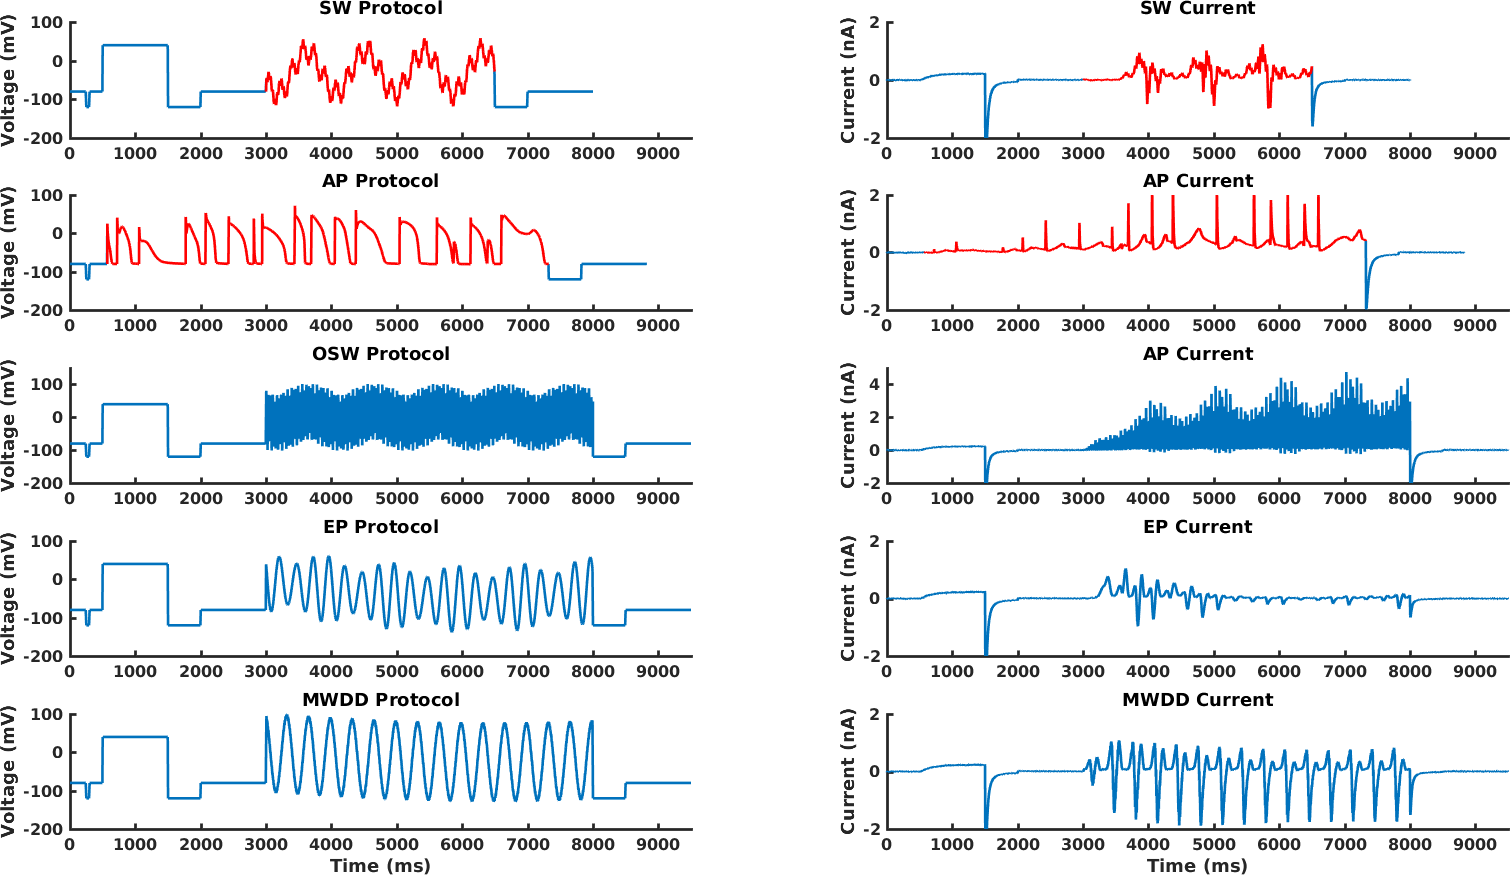
\includegraphics[scale=0.42]{Figures/Protocols.png}
\caption{\textbf{Protocols and current traces used in this report.} All five protocols and the resulting current traces for cell 16713110 as used in this study are shown with capacitative spikes removed. For the SW and AP protocols, the `core' of the protocol used in Sections \ref{SubSec_Lasso_Discrepancy} and \ref{SubSec_StepwiseLM_Discrepancy} are highlighted in red. Note that the y-axis scale for the OSW protocol and current differ from the other protocols due to the higher (and non-physiological) potentials reached - this was one reason for the rejection of the OSW protocol during the development of the SW protocol.}
\label{Fig_Protocols}
\end{center}
\end{figure}

\subsection{Predicting Discrepancy Using LASSO}\label{SubSec_Lasso_Discrepancy}

\subsubsection{The Method}
The Least Absolute Shrinkage and Selection Operator (LASSO)\footnote{\url{https://www.mathworks.com/help/stats/lasso.html}} is a popular linear regression method that incorporates a regularization parameter $\lambda$. For a set of predictors $X$, $N$ data points $y$ and coefficients $\beta$, the LASSO method can be written in Lagrangian form as
\begin{align}
	\min_{\beta} ( \frac{1}{N} \norm{ y - \beta X }^2 + \lambda \norm{ \beta }^1 ).
\end{align}
The size of the parameter $\lambda$ determines the degree of regularization. Essentially, a large $\lambda$ penalizes $\beta$ heavily, and so produces smaller models. Conversely, a small $\lambda$ allows the method more freedom in the number of variables included. A key feature of the LASSO algorithm is that due to the $L_1$ norm used for regularization, elements of $\beta$ can be set to zero by the method, resulting in smaller models. This key property has made LASSO a popular method in Machine Learning. Variations on this method are Ridge regression (uses $\lambda \norm{ \beta }^2$ instead) and Elastic Net regression (a combination of Ridge and LASSO).

One challenge of the LASSO method is that there is no a priori choice for the regularization parameter $\lambda$. To determine $\lambda$ and check the validity of the resulting models we use K-fold cross-validation. This method works by splitting the experimental data into K equally sized folds, leaving one out, then checking the model's ability to predict the data in the left out fold. This results in a mean squared error (MSE) for each fold, and for each value of $\lambda$. The variation in the MSE at each $lambda$ can be used to select $\lambda$ and hence, the model. To do so, we find the $\lambda$ value giving the minimum MSE, and then choose the largest $\lambda$ within one standard deviation from this point. This can be seen as choosing the smallest justifiable  model within the variation of the model that gives the absolute minium error. In this study, we use 10 folds which is a fairly standard choice.

An important property of K-fold cross-validation as inplemented in Matlab is that it uses random data points in each fold. While this is in principle a good thing, the extremely high time resolution of our data means that all of the resulting folds are likely to be effectively the same, subject to experimental noise. As a result, the models produced by the Matlab algorithm were both non-predictive and non-deterministic. To correct for this phenomenon and produce meaningful folds, some editing of the Matlab source code is required (detailed in README.md). We instead split the trace into ten equal segments consecutive in time to ensure variation between folds.

\subsubsection{Results}

LASSO fits for a linear regression model of model discrepancy of $d$ and $d_o$ are shown in Figure \ref{Fig_LASSO_SW_AP_full_discrepancy}. For this model, the discrepancies resulting from the sine wave (SW) protocol developed in by Beattie et al.~was used as training data, and was used to predict the results from the action potential (AP) protocol used for validation in that study. The resulting corrected currents together with the original simulation and experimental data are shown in Fig.~\ref{Fig_LASSO_SW_AP_full_currents}. It can be appreciated that, in both cases, the linear models of discrepancy fail to predict the discrepancy observed in the AP trace.

\begin{figure}[t]
\begin{center}
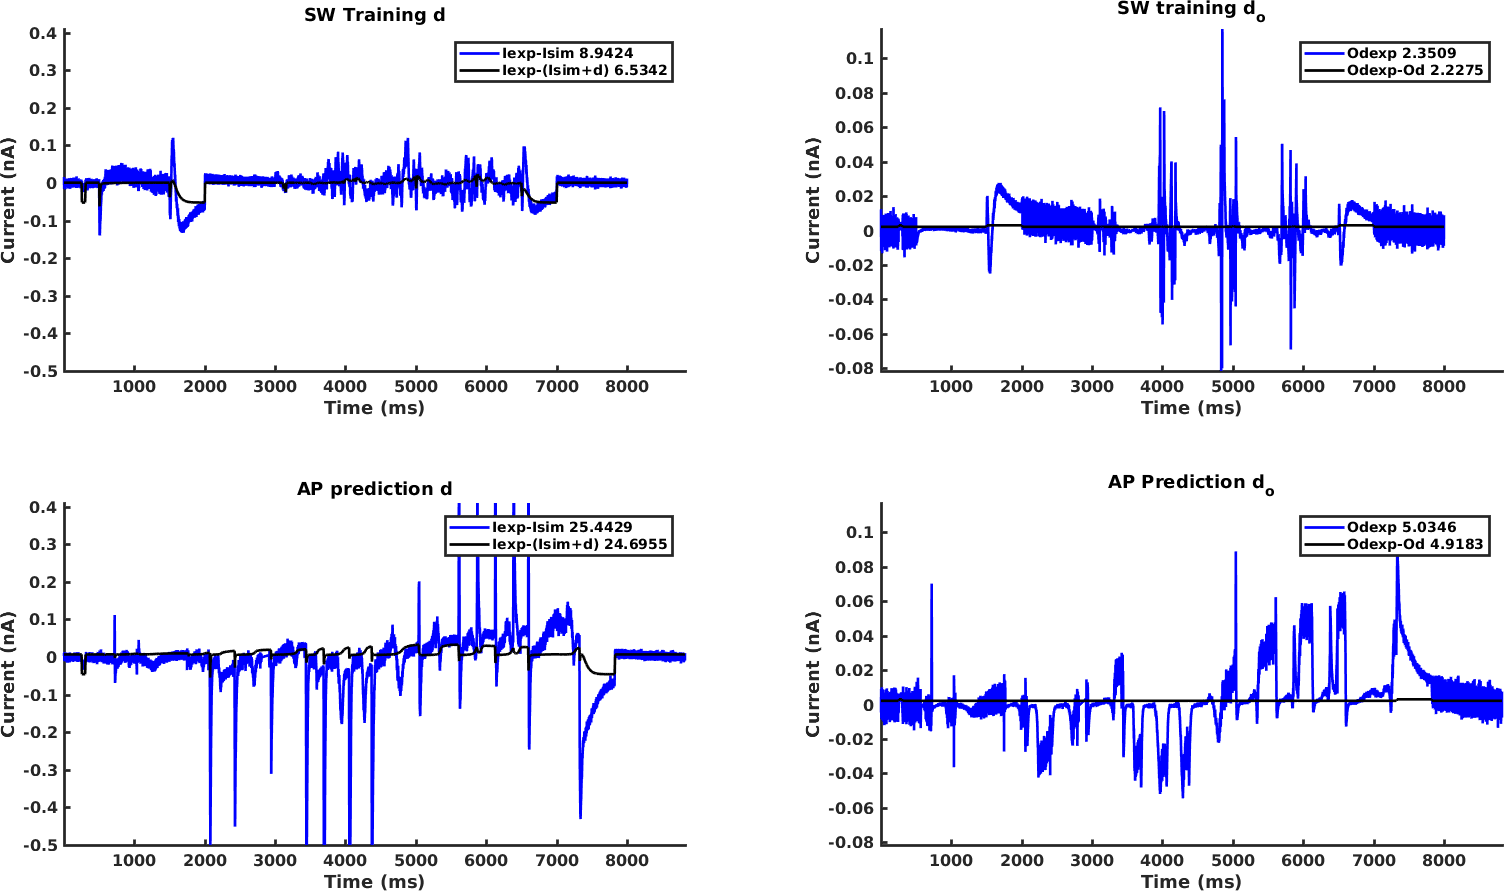
\includegraphics[scale=0.42]{Figures/LASSO_SW_AP_full_discrepancy.png}
\caption{\textbf{Linear model of discrepancy constructed using LASSO from the SW protocol.} These models of $d$ (left) and $d_o$ (right) were constructed using LASSO on the entire SW trace (top), starting with all linearly independent predictors. The improvement of the training trace (top) is poor and the resulting models fail to predict the discrepancy in the AP trace (bottom). The root mean square errors between the simulated and predicted traces are shown in the legends. } 
\label{Fig_LASSO_SW_AP_full_discrepancy}
\end{center}
\end{figure}

\begin{figure}[hb]
\begin{center}
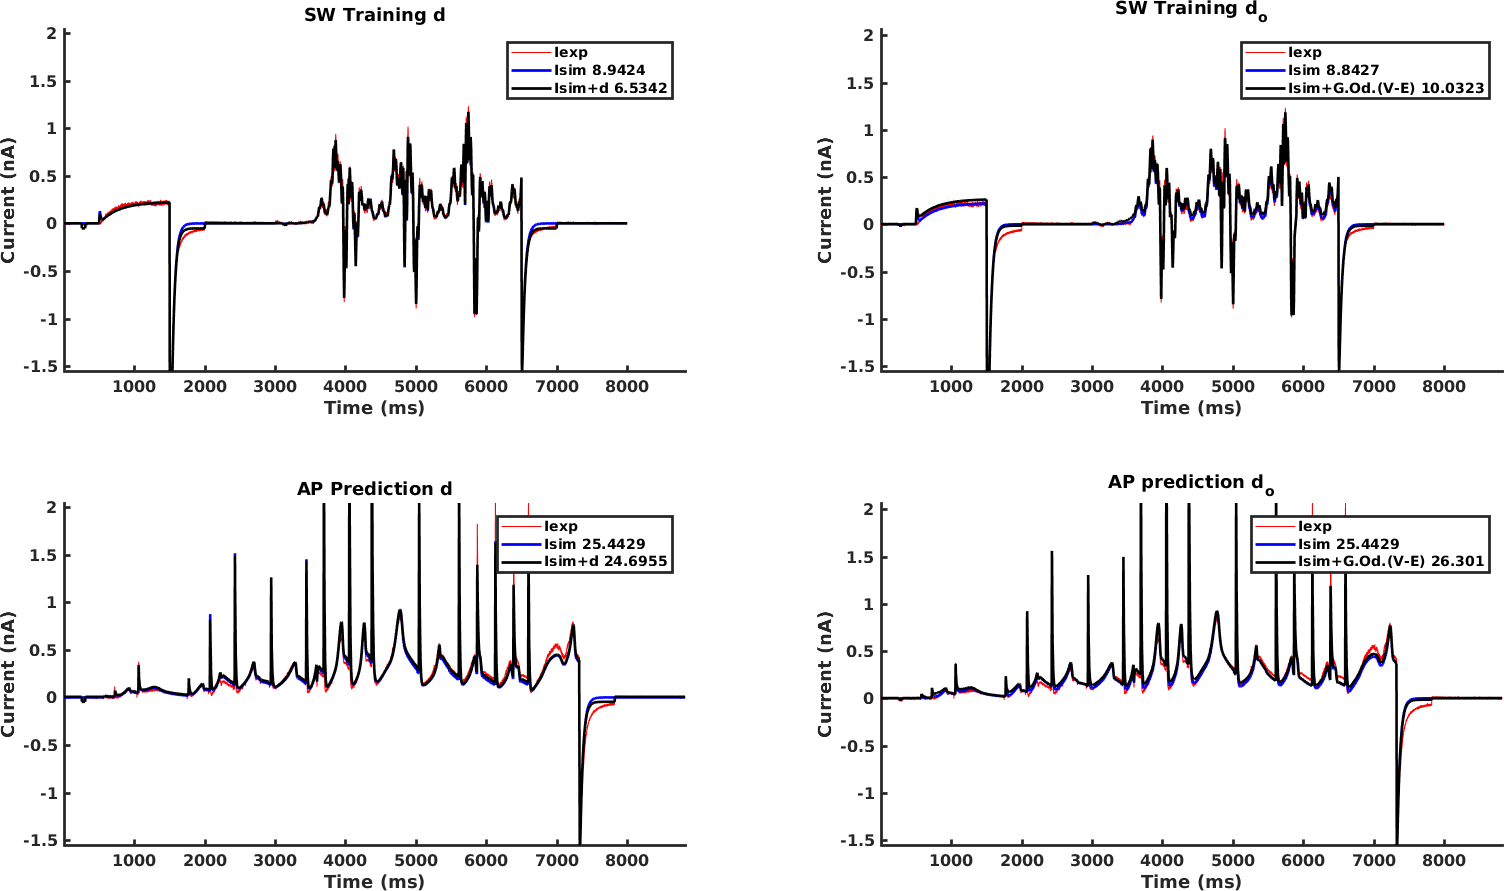
\includegraphics[scale=0.42]{Figures/LASSO_SW_AP_full_currents.png}
\caption{\textbf{Corrected currents using a linear model of discrepancy constructed using LASSO from the SW protocol.} The models of $d$ (left) and $d_o$ (right) in Fig. ~\ref{Fig_LASSO_SW_AP_full_discrepancy} have been incorporated into the simulation (blue line), giving a revised prediction for the SW and AP protocols (black line). As expected from Fig.~\ref{Fig_LASSO_SW_AP_full_discrepancy}, there is little improvement in the agreement with the experimental data (red line). The sum of squared errors between the models and the data are shown in the legend.}
\label{Fig_LASSO_SW_AP_full_currents}
\end{center}
\end{figure}

Included parameters and their coefficients are shown in Fig.~\ref{Fig_LASSO_SW_AP_coefficients}. The parameters differ considerably between the models for $d$ and $d_o$. Fig.~\ref{Fig_LASSO_SW_AP_lambda} shows the plot of $\lambda$ as a function of MSE. The model with the minimum MSE is indicated by the green line and the model with the largest value of $\lambda$ (hence, the smallest model) within one standard error of the minimum MSE model is shown by the blue line. Note the characteristic U-shaped form of the $\lambda$ - MSE relationship, with overfitting on the right and underfitting on the left.

\begin{figure}[t]
\begin{center}
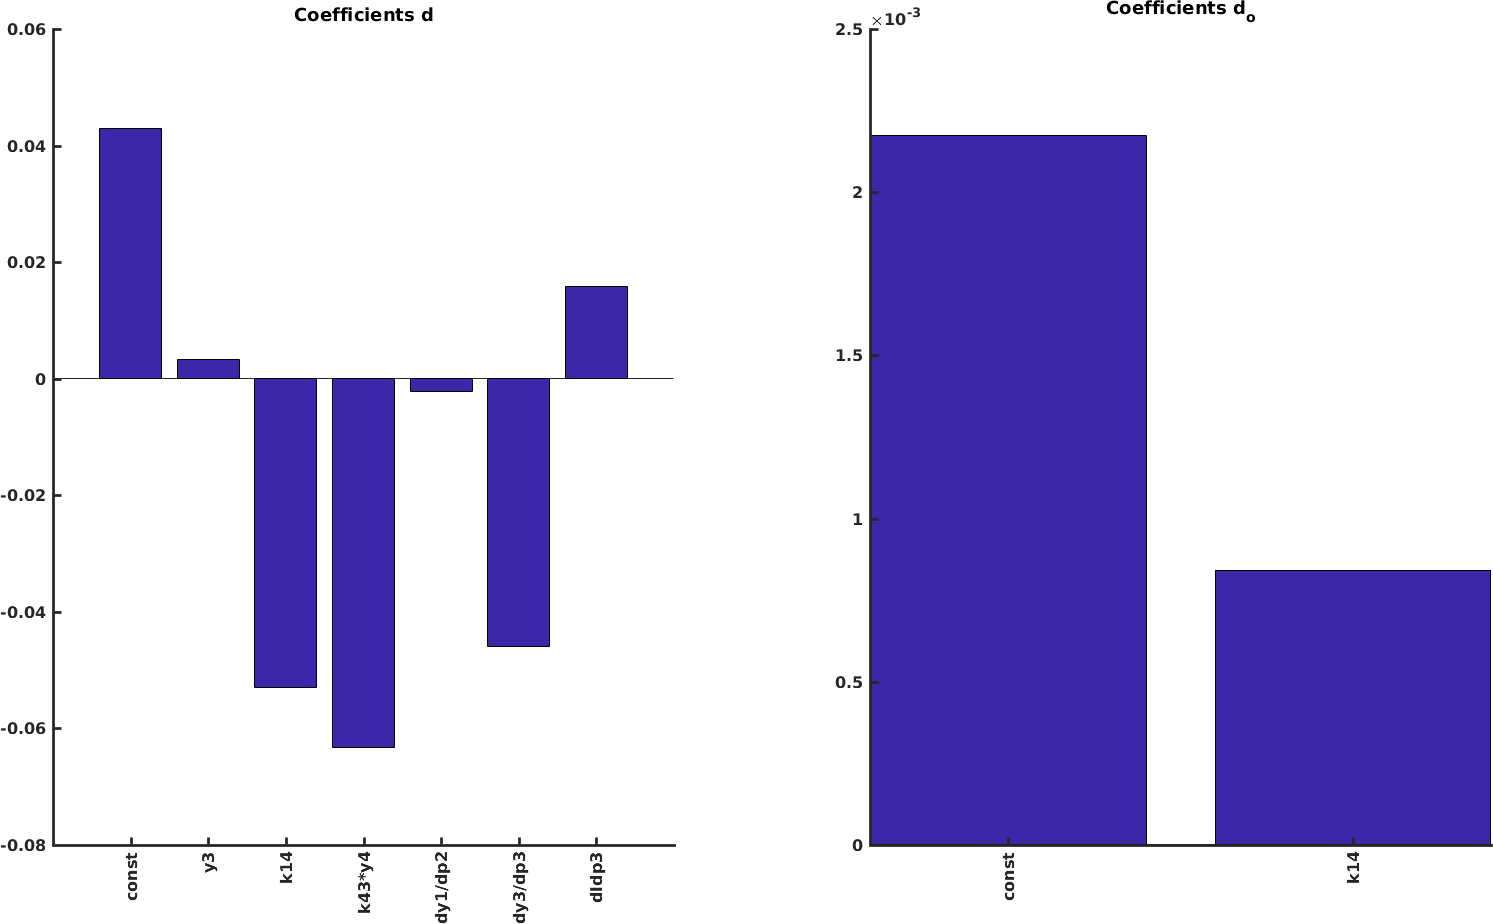
\includegraphics[scale=0.42]{Figures/LASSO_SW_AP_full_coefficients.png}
\caption{\textbf{Coefficients in the linear model of discrepancy constructed using LASSO from the SW protocol.} This plot shows the included parameters and coefficients for the model produced by LASSO shown in Fig.~\ref{Fig_LASSO_SW_AP_full_discrepancy} and Fig.~\ref{Fig_LASSO_SW_AP_full_currents}. Coefficients for $d$ are shown on the left, and coefficients for $d_o$ are shown on the right.} 
\label{Fig_LASSO_SW_AP_coefficients}
\end{center}
\end{figure}

\begin{figure}[hb]
\begin{center}
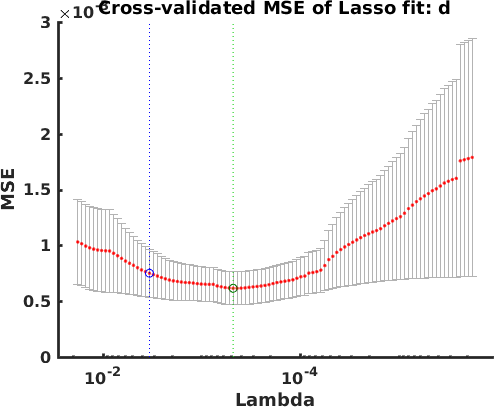
\includegraphics[scale=0.42]{Figures/LASSO_SW_AP_full_lambda_d.png}
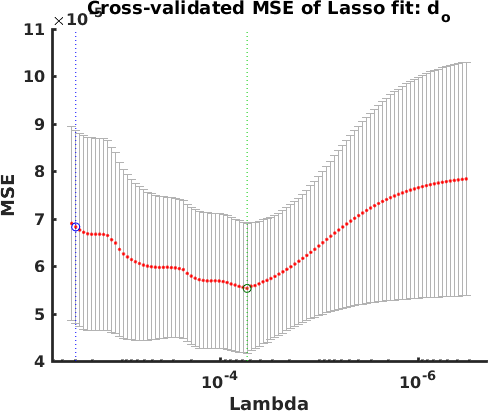
\includegraphics[scale=0.42]{Figures/LASSO_SW_AP_full_lambda_od.png}
\caption{\textbf{$\lambda$ and Mean Squared Error plots from the linear models of the SW protocol.} The models of $d$ (left) and $d_o$ (right) have been generated by varying $\lambda$. The error bars indicate the standard error in the MSE between folds. The value of $\lambda$ giving the minimum MSE is indicated by the green line and the selected value of $\lambda$, being the largest value of $\lambda$ with an MSE within one standard error of the minimum, is shown in blue. Note that $\lambda$ runs from largest to smallest, so that the largest model is on the left.}
\label{Fig_LASSO_SW_AP_lambda}
\end{center}
\end{figure}

\clearpage

Based on the failure of the `naive' LASSO method in this standard case, we also addressed the following hypotheses:
\begin{itemize}
\item the LASSO method might be biased by the large errors that occur in the deactivation steps, and so fail to fit the more subtle errors in the main part of the trace.
\item Because the fit to the SW protocol is `optimal' and  extremely good, there may simply not be enough information in the discrepancy of the sine wave protocol to train a model.
\end{itemize}

To address the first hypothesis, we tried fitting a model to only the sine wave generated part of the SW protocol, and omit the activation and deactivation steps on either end (see Fig.~\ref{Fig_Protocols}). These were then used to predict only the section of the AP protocol containing the action potentials. To address the second hypothesis, we instead trained the models using alternative protocols (OSW, EP, MWDD) that were recorded during the course of the sine wave protocol study. Results for each of these approaches are shown in Fig.~\ref{Fig_LASSO_SW_AP_core_discrepancy}-\ref{Fig_LASSO_AP_AP_full_lambda}. In each case, the linear model of discrepancy only provides marginal gains in the training data, and either fails to improve the discrepancy in the prediction (AP) trace or makes it worse. In general, across all sets of results, the discrepancy in the open probability, $d_o$, appears to be both harder to predict and lead to more over-fitting than the standard definition, $d$.

To investigate what the `best possible' model would look like, we also constructed a model from our prediction data, namely the discrepancy in the AP protocol. The quality of this fit effectively places an upper bound on the success of the LASSO procedure for constructing a linear model of the data we wish to predict. This model is shown in Figs.~\ref{Fig_LASSO_SW_AP_core_discrepancy}-\ref{Fig_LASSO_OSW_AP_core_lambda}. Whilst this model produces an appreciable improvement in the agreement between data and model, this result suggests that a linear regression approach would only ever be able to account for a sub-portion of the discrepancy observed between simulation and experiment.

\begin{figure}[t]
\begin{center}
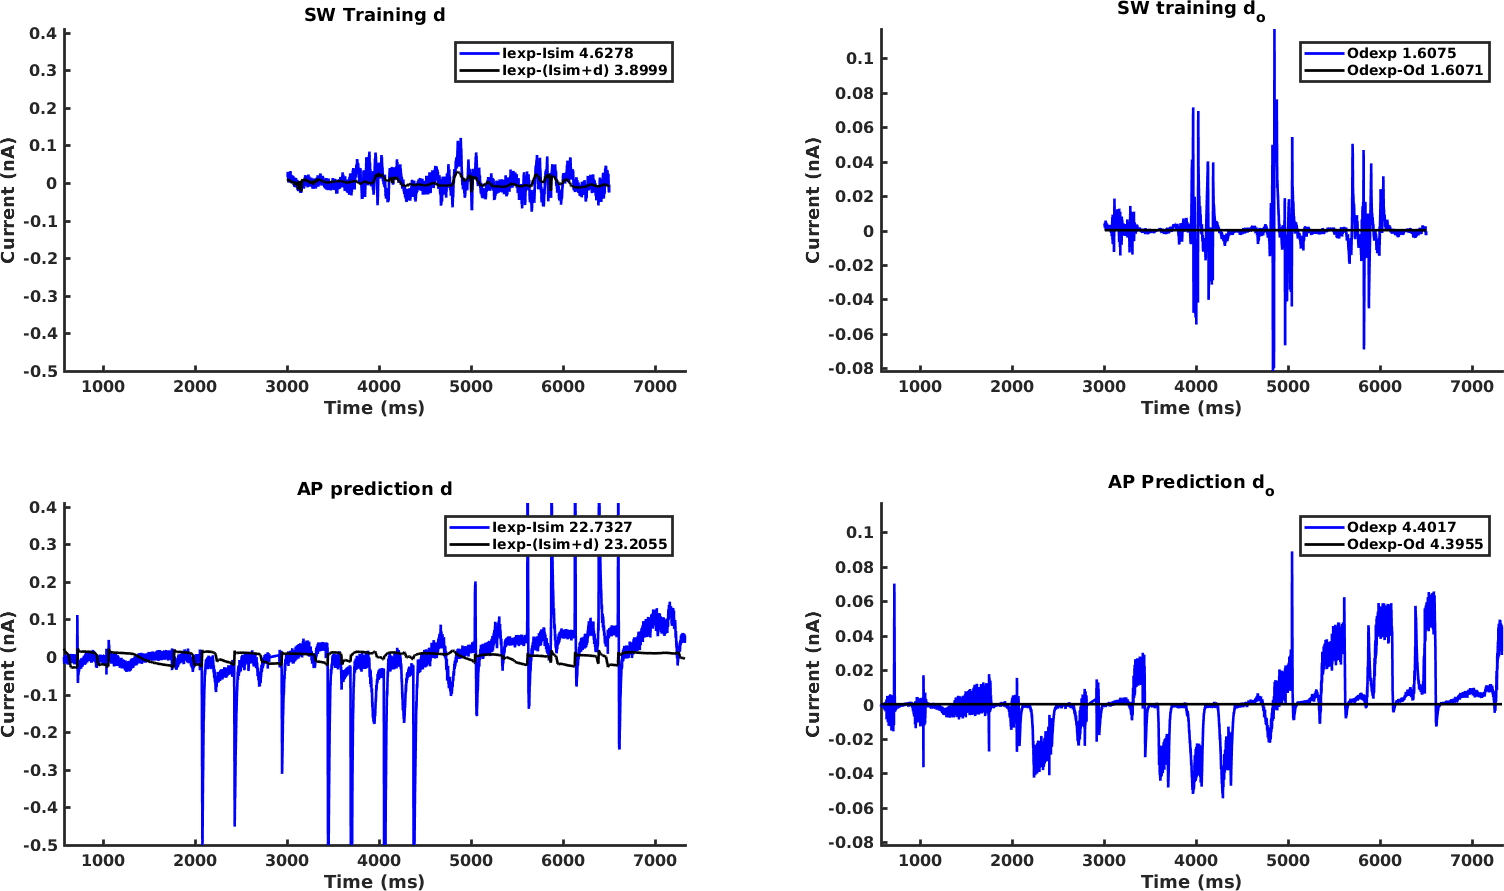
\includegraphics[scale=0.42]{Figures/LASSO_SW_AP_core_discrepancy.png}
\caption{\textbf{Linear model of discrepancy constructed using LASSO.} These models of $d$ (left) and $d_o$ (right) were constructed using LASSO on the entire SW trace (top), starting with all linearly independent predictors. The root mean square errors between the simulated and predicted traces are shown in the legends. } 
\label{Fig_LASSO_SW_AP_core_discrepancy}
\end{center}
\end{figure}

\begin{figure}[hb]
\begin{center}
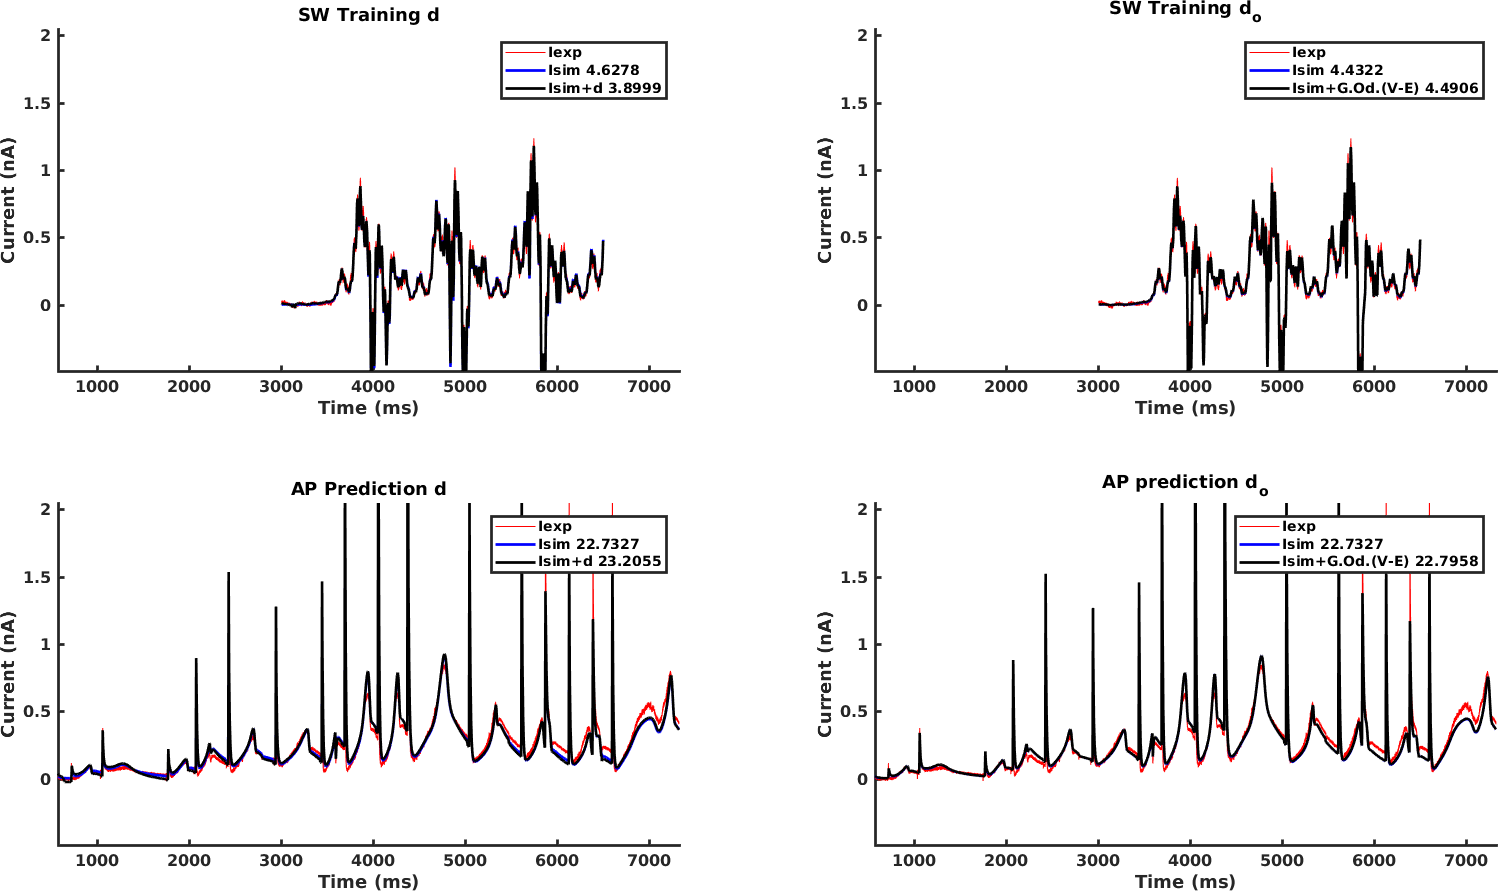
\includegraphics[scale=0.42]{Figures/LASSO_SW_AP_core_currents.png}
\caption{\textbf{Corrected currents using a linear model of discrepancy constructed using LASSO from the sine wave generated component of the SW protocol.} The models of $d$ (left) and $d_o$ (right) in Fig.~\ref{Fig_LASSO_SW_AP_core_discrepancy} have been incorporated into the simulation (blue line), giving a revised prediction for the SW and AP protocols (black line). The sum of squared errors between the models and the data are shown in the legend.}
\label{Fig_LASSO_SW_AP_core_currents}
\end{center}
\end{figure}

\clearpage

\begin{figure}[t]
\begin{center}
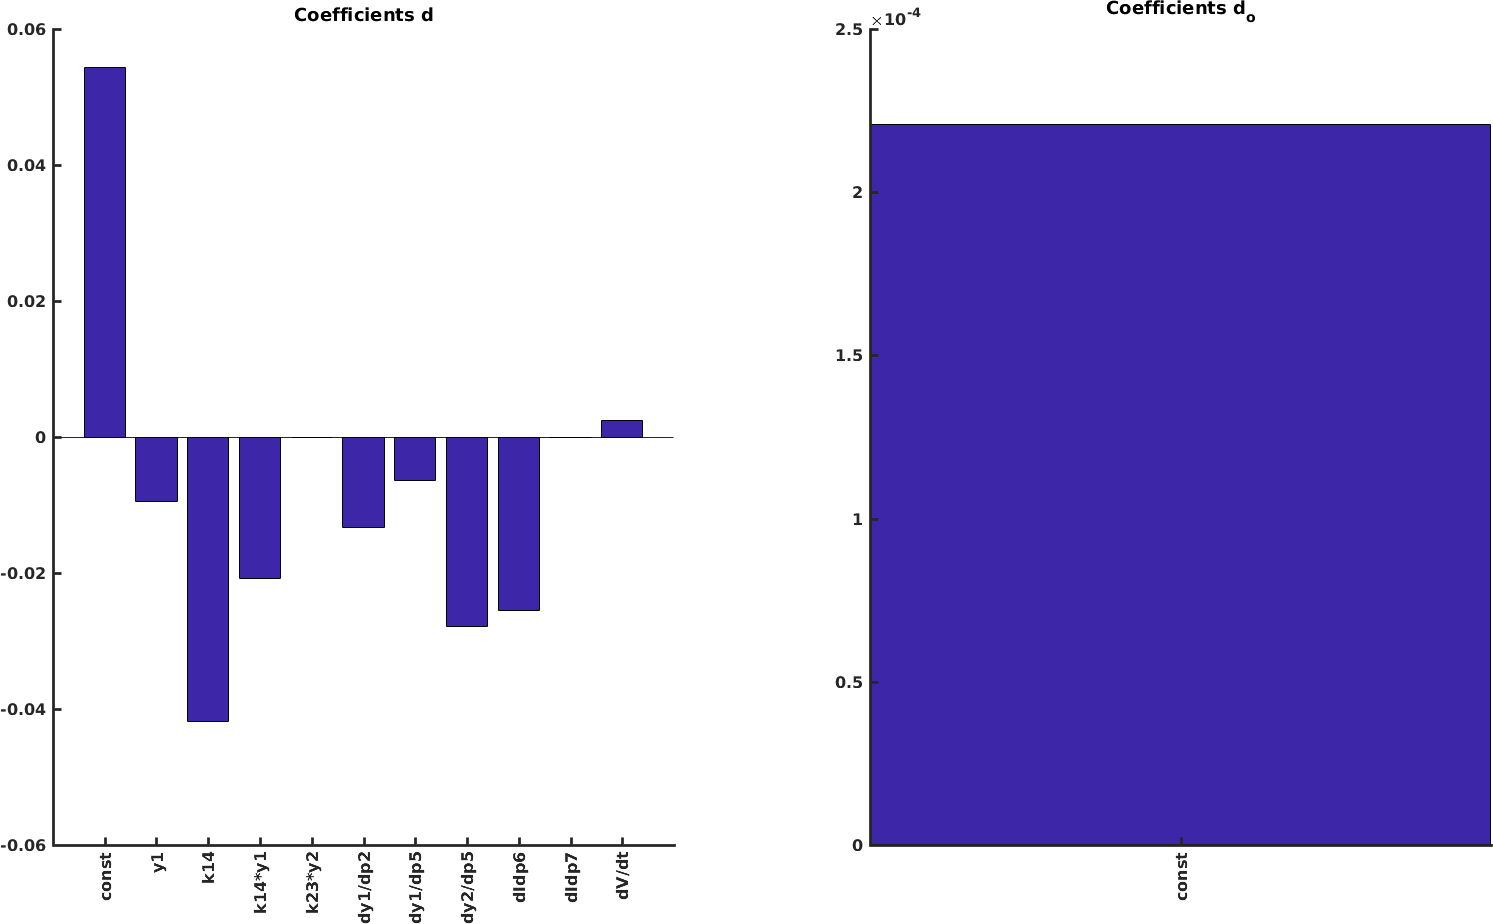
\includegraphics[scale=0.42]{Figures/LASSO_SW_AP_core_coefficients.png}
\caption{\textbf{Coefficients in the linear model of discrepancy constructed using LASSO from the sine wave generated component of the SW protocol.} This plot shows the included parameters and coefficients for the model produced by LASSO shown in Fig.~\ref{Fig_LASSO_SW_AP_core_discrepancy} and Fig.~\ref{Fig_LASSO_SW_AP_core_currents}. Coefficients for $d$ are shown on the left, and coefficients for $d_o$ are shown on the right.} 
\label{Fig_LASSO_SW_AP_core_coefficients}
\end{center}
\end{figure}

\begin{figure}[hb]
\begin{center}
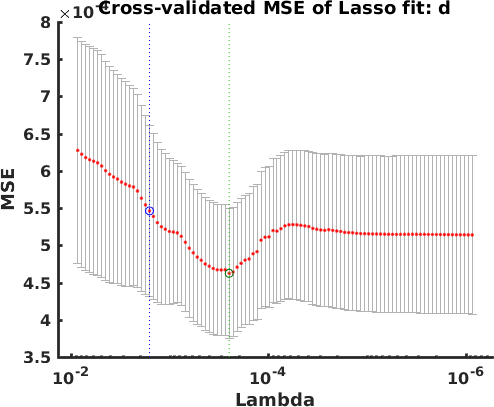
\includegraphics[scale=0.42]{Figures/LASSO_SW_AP_core_lambda_d.png}
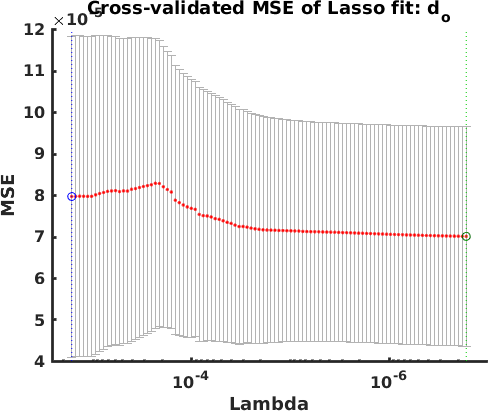
\includegraphics[scale=0.42]{Figures/LASSO_SW_AP_core_lambda_od.png}
\caption{\textbf{$\lambda$ and Mean Squared Error plots from the linear models of the sine wave component of the SW protocol.} The models of $d$ (left) and $d_o$ (right) have been generated by varying $\lambda$. The error bars indicate the standard error in the MSE between folds. The value of $\lambda$ giving the minimum MSE is indicated by the green line and the selected value of $\lambda$, being the largest value of $\lambda$ with an MSE within one standard error of the minimum, is shown in blue. Note that $\lambda$ runs from largest to smallest, so that the largest model is on the left.}
\label{Fig_LASSO_SW_AP_core_lambda}
\end{center}
\end{figure}

\clearpage

\begin{figure}[t]
\begin{center}
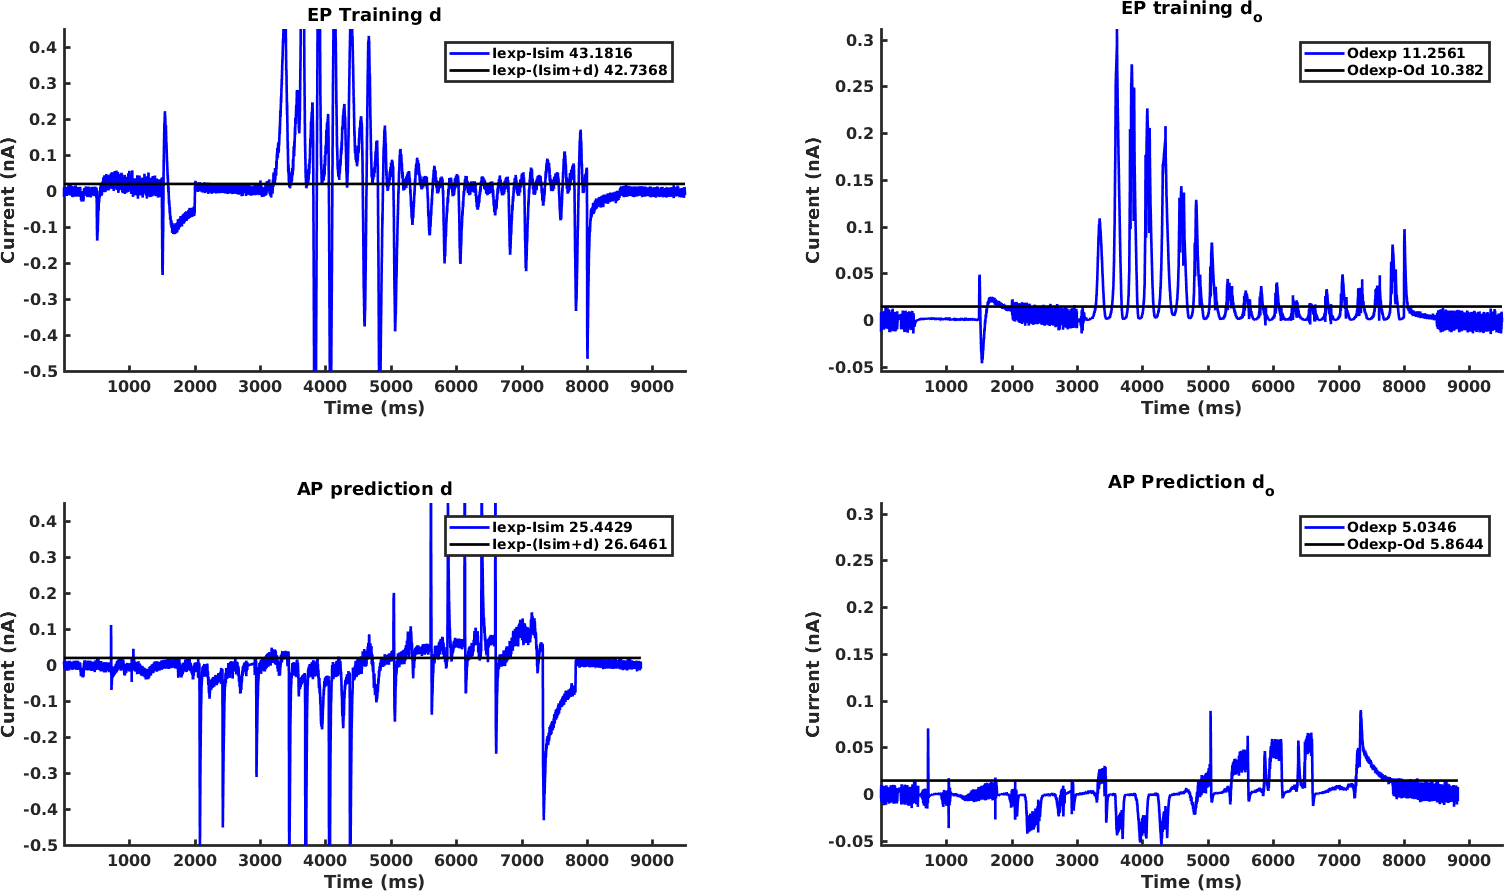
\includegraphics[scale=0.42]{Figures/LASSO_EP_AP_full_discrepancy.png}
\caption{\textbf{Linear model of discrepancy constructed using LASSO from the EP protocol.} These models of $d$ (left) and $d_o$ (right) were constructed using LASSO on the entire SW trace (top), starting with all linearly independent predictors. The root mean square errors between the simulated and predicted traces are shown in the legends. } 
\label{Fig_LASSO_EP_AP_full_discrepancy}
\end{center}
\end{figure}

\begin{figure}[hb]
\begin{center}
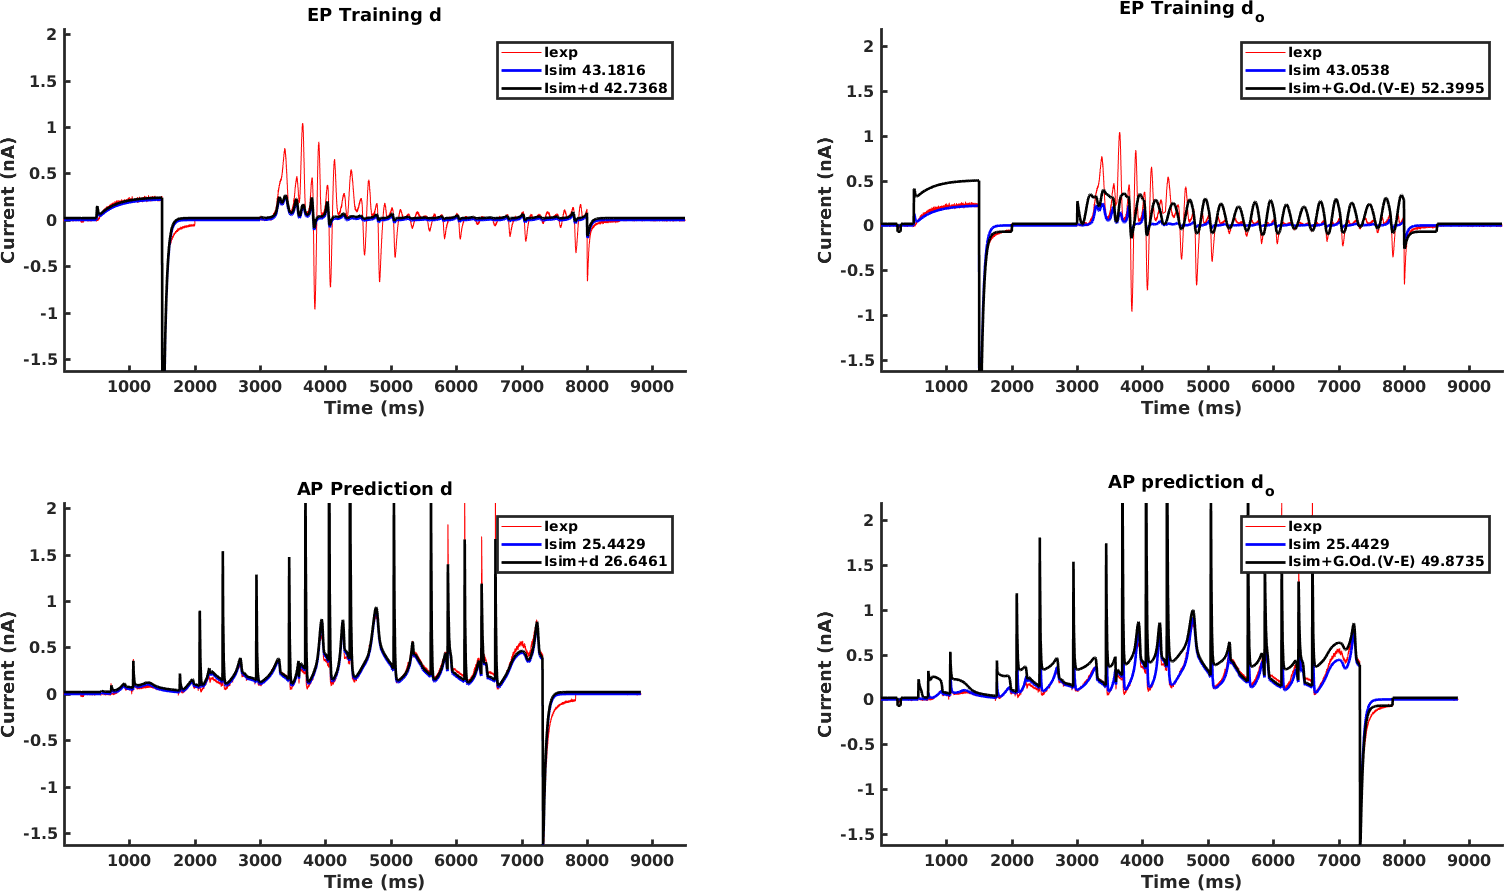
\includegraphics[scale=0.42]{Figures/LASSO_EP_AP_full_currents.png}
\caption{\textbf{Corrected currents using a linear model of discrepancy constructed using LASSO from the EP protocol.} The models of $d$ (left) and $d_o$ (right) in Fig. ~\ref{Fig_LASSO_SW_AP_full_discrepancy} have been incorporated into the simulation (blue line), giving a revised prediction for the EP and AP protocols (black line). The sum of squared errors between the models and the data are shown in the legend.}
\label{Fig_LASSO_EP_AP_full_currents}
\end{center}
\end{figure}

\clearpage

\begin{figure}[t]
\begin{center}
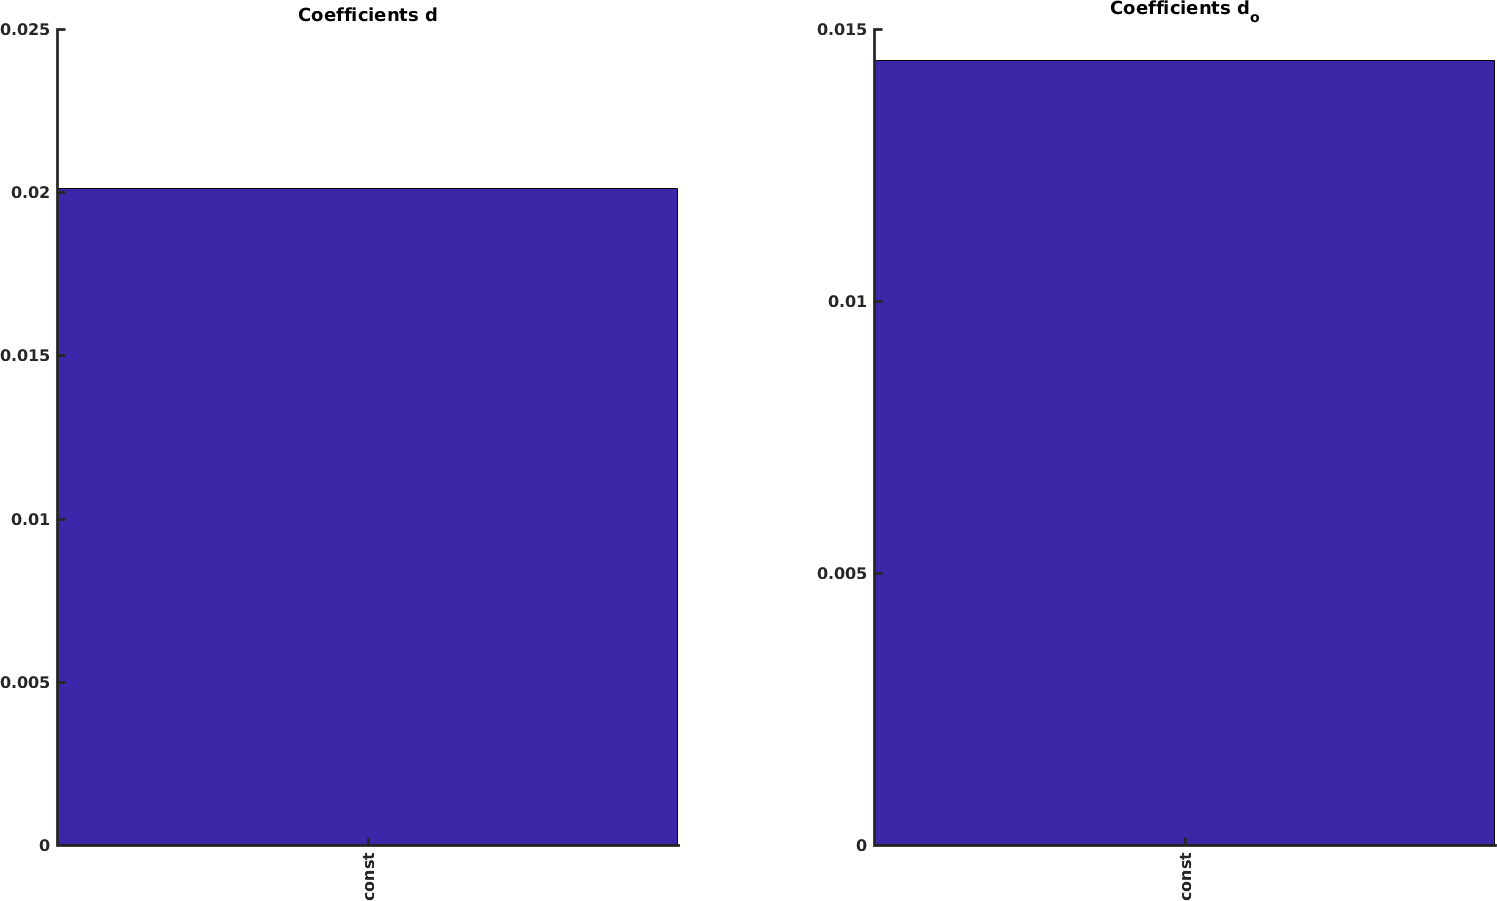
\includegraphics[scale=0.42]{Figures/LASSO_EP_AP_full_coefficients.png}
\caption{\textbf{Coefficients in the linear model of discrepancy constructed using LASSO from the sine wave generated component of the EP protocol.} This plot shows the included parameters and coefficients for the model produced by LASSO shown in Fig.~\ref{Fig_LASSO_EP_AP_full_discrepancy} and Fig.~\ref{Fig_LASSO_EP_AP_full_currents}. Coefficients for $d$ are shown on the left, and coefficients for $d_o$ are shown on the right.} 
\label{Fig_LASSO_EP_AP_full_coefficients}
\end{center}
\end{figure}

\begin{figure}[hb]
\begin{center}
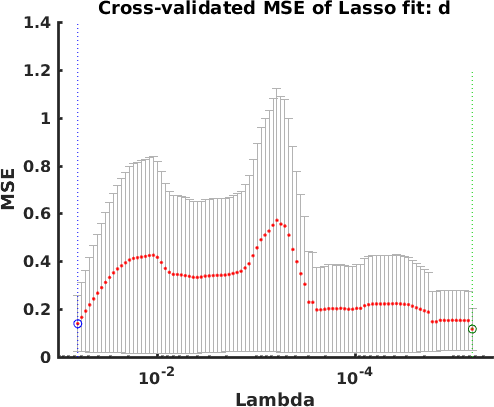
\includegraphics[scale=0.42]{Figures/LASSO_EP_AP_full_lambda_d.png}
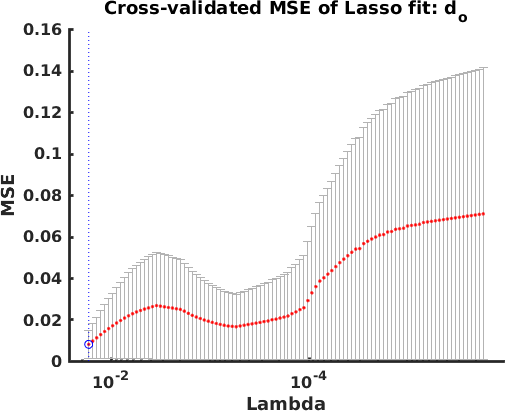
\includegraphics[scale=0.42]{Figures/LASSO_EP_AP_full_lambda_od.png}
\caption{\textbf{$\lambda$ and Mean Squared Error plots from the linear models of the sine wave component of the EP protocol.} The models of $d$ (left) and $d_o$ (right) have been generated by varying $\lambda$. The error bars indicate the standard error in the MSE between folds. The value of $\lambda$ giving the minimum MSE is indicated by the green line and the selected value of $\lambda$, being the largest value of $\lambda$ with an MSE within one standard error of the minimum, is shown in blue. Note that $\lambda$ runs from largest to smallest, so that the largest model is on the left.}
\label{Fig_LASSO_EP_AP_full_lambda}
\end{center}
\end{figure}

\clearpage

\begin{figure}[t]
\begin{center}
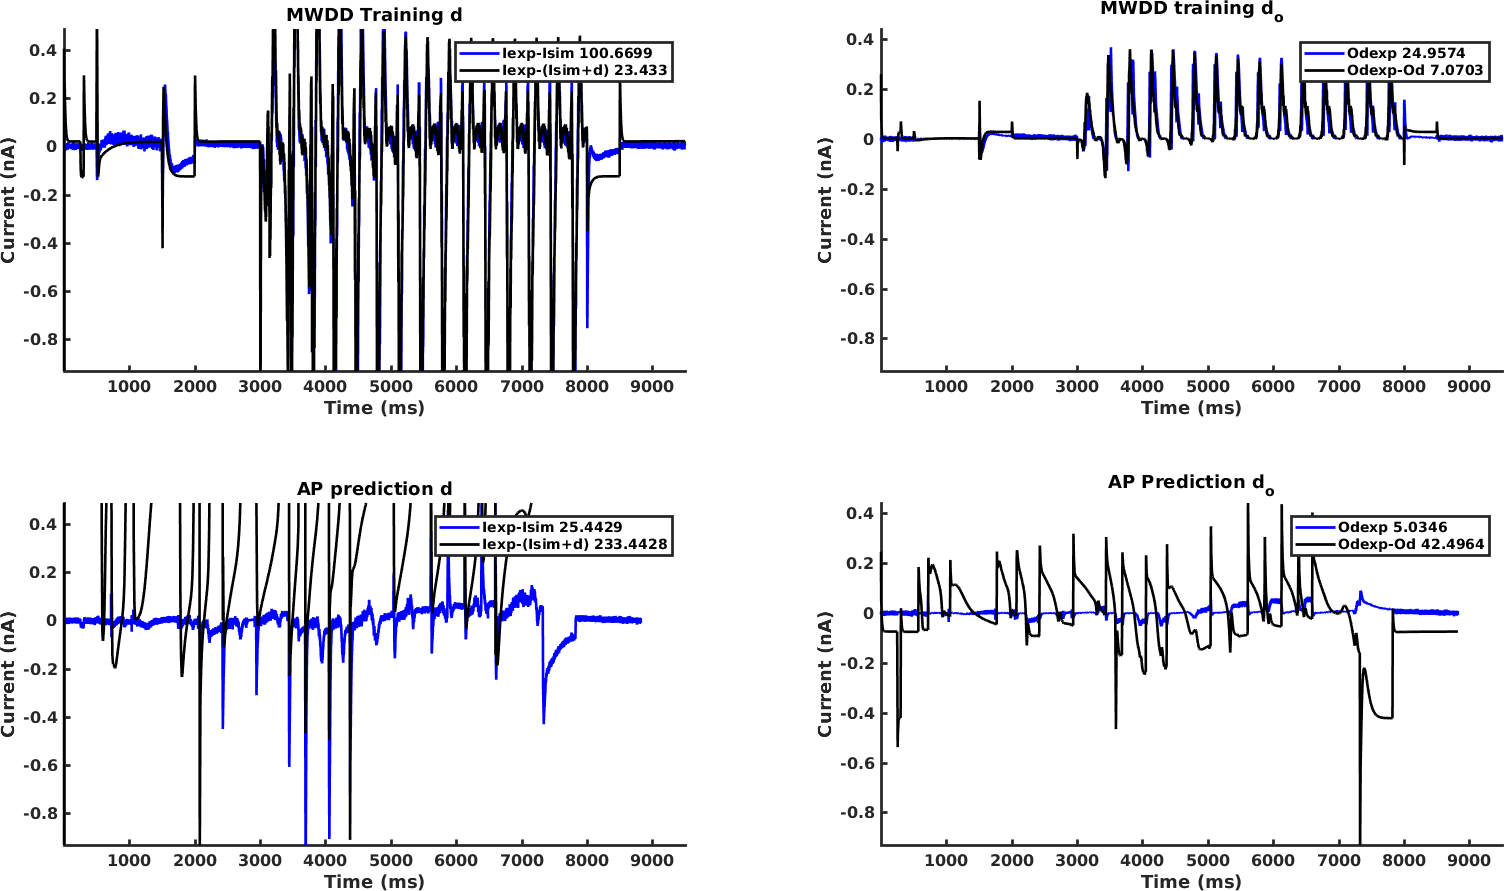
\includegraphics[scale=0.42]{Figures/LASSO_MWDD_AP_full_discrepancy.png}
\caption{\textbf{Linear model of discrepancy constructed using LASSO from the MWDD protocol.} These models of $d$ (left) and $d_o$ (right) were constructed using LASSO on the entire MWDD trace (top), starting with all linearly independent predictors. The root mean square errors between the simulated and predicted traces are shown in the legends. } 
\label{Fig_LASSO_MWDD_AP_full_discrepancy}
\end{center}
\end{figure}

\begin{figure}[hb]
\begin{center}
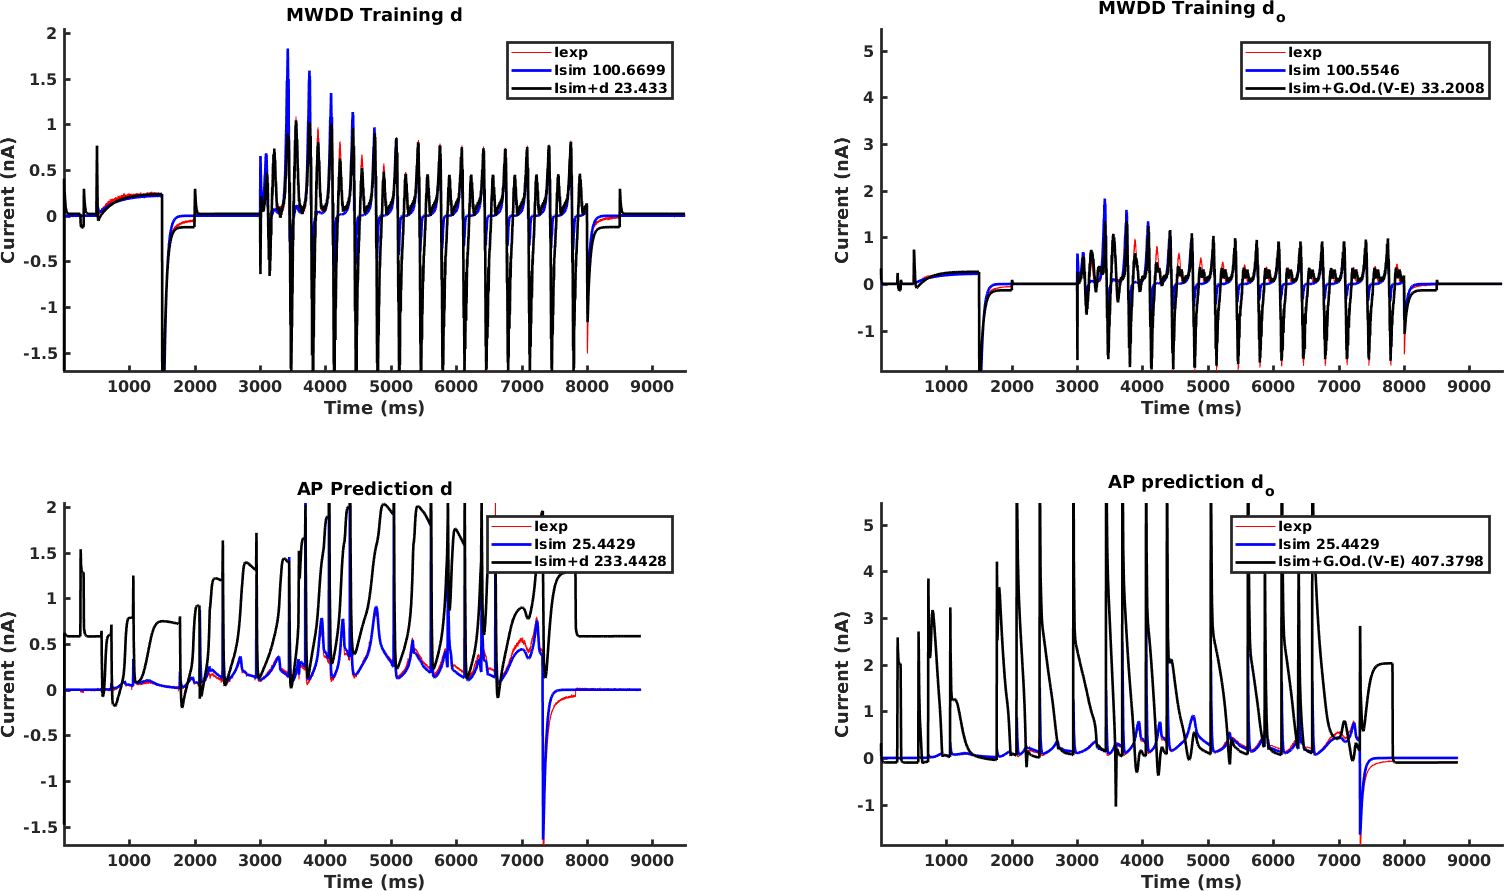
\includegraphics[scale=0.42]{Figures/LASSO_MWDD_AP_full_currents.png}
\caption{\textbf{Corrected currents using a linear model of discrepancy constructed using LASSO from the MWDD protocol.} The models of $d$ (left) and $d_o$ (right) in Fig. ~\ref{Fig_LASSO_MWDD_AP_full_discrepancy} have been incorporated into the simulation (blue line), giving a revised prediction for the MWDD and AP protocols (black line). The sum of squared errors between the models and the data are shown in the legend.}
\label{Fig_LASSO_MWDD_AP_full_currents}
\end{center}
\end{figure}

\clearpage

\begin{figure}[t]
\begin{center}
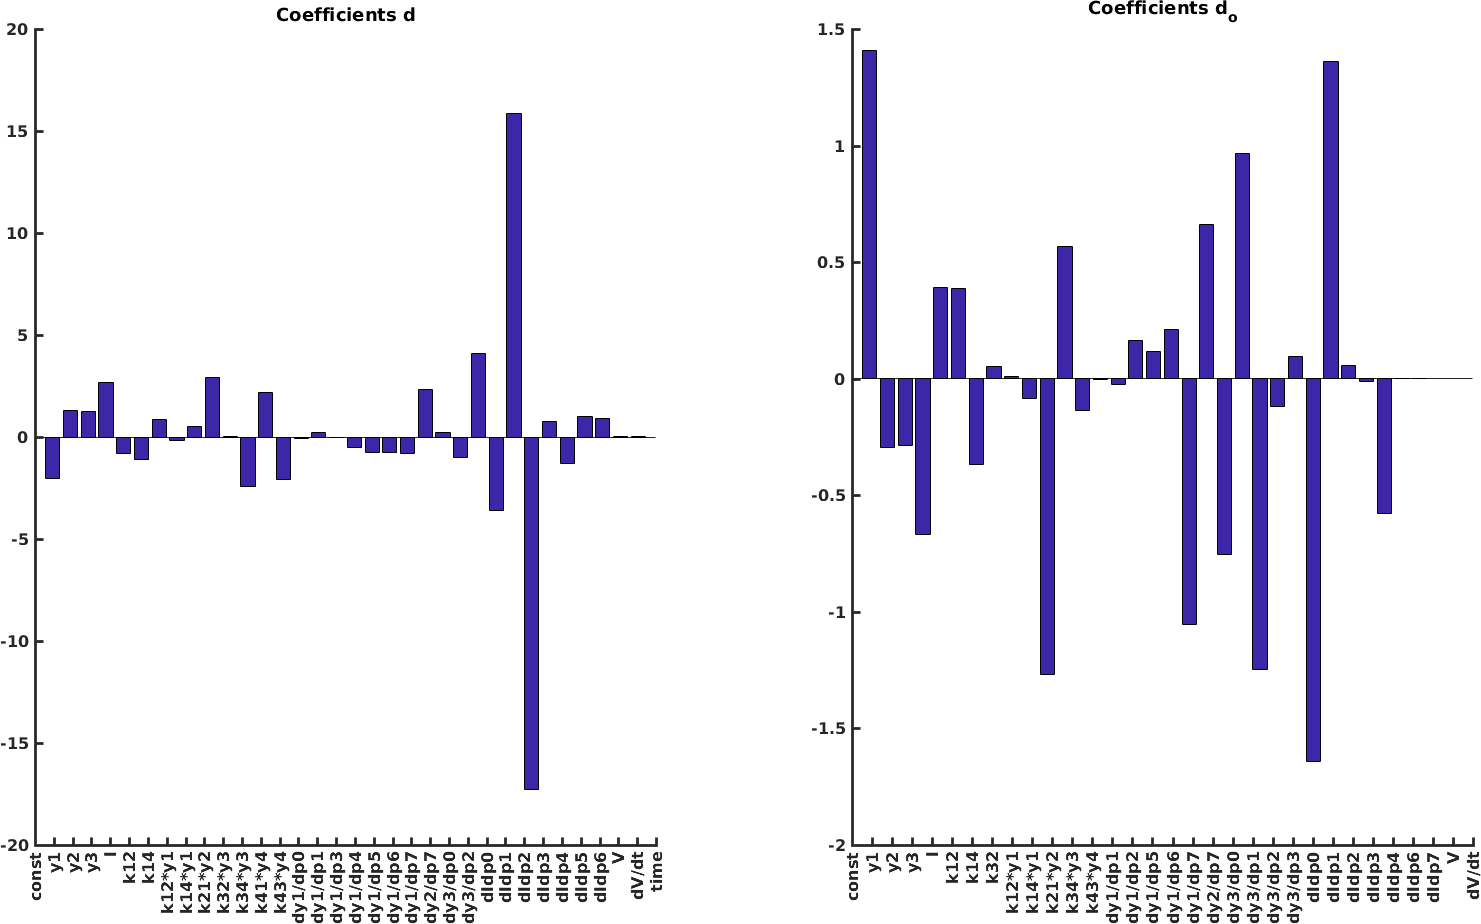
\includegraphics[scale=0.42]{Figures/LASSO_MWDD_AP_full_coefficients.png}
\caption{\textbf{Coefficients in the linear model of discrepancy constructed using LASSO from the sine wave generated component of the MWDD protocol.} This plot shows the included parameters and coefficients for the model produced by LASSO shown in Fig.~\ref{Fig_LASSO_MWDD_AP_full_discrepancy} and Fig.~\ref{Fig_LASSO_MWDD_AP_full_currents}. Coefficients for $d$ are shown on the left, and coefficients for $d_o$ are shown on the right.} 
\label{Fig_LASSO_MWDD_AP_full_coefficients}
\end{center}
\end{figure}

\begin{figure}[hb]
\begin{center}
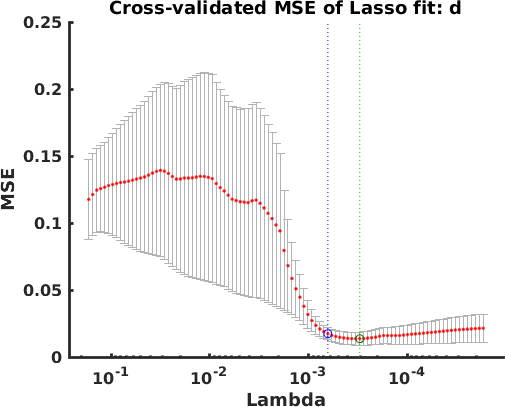
\includegraphics[scale=0.42]{Figures/LASSO_MWDD_AP_full_lambda_d.png}
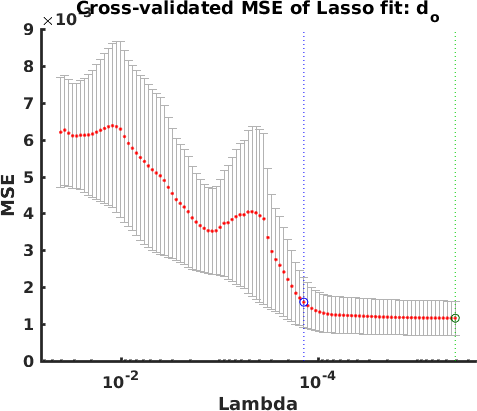
\includegraphics[scale=0.42]{Figures/LASSO_MWDD_AP_full_lambda_od.png}
\caption{\textbf{$\lambda$ and Mean Squared Error plots from the linear models of the sine wave component of the MWDD protocol.} The models of $d$ (left) and $d_o$ (right) have been generated by varying $\lambda$. The error bars indicate the standard error in the MSE between folds. The value of $\lambda$ giving the minimum MSE is indicated by the green line and the selected value of $\lambda$, being the largest value of $\lambda$ with an MSE within one standard error of the minimum, is shown in blue. Note that $\lambda$ runs from largest to smallest, so that the largest model is on the left.}
\label{Fig_LASSO_MWDD_AP_full_lambda}
\end{center}
\end{figure}

\clearpage

\begin{figure}[t]
\begin{center}
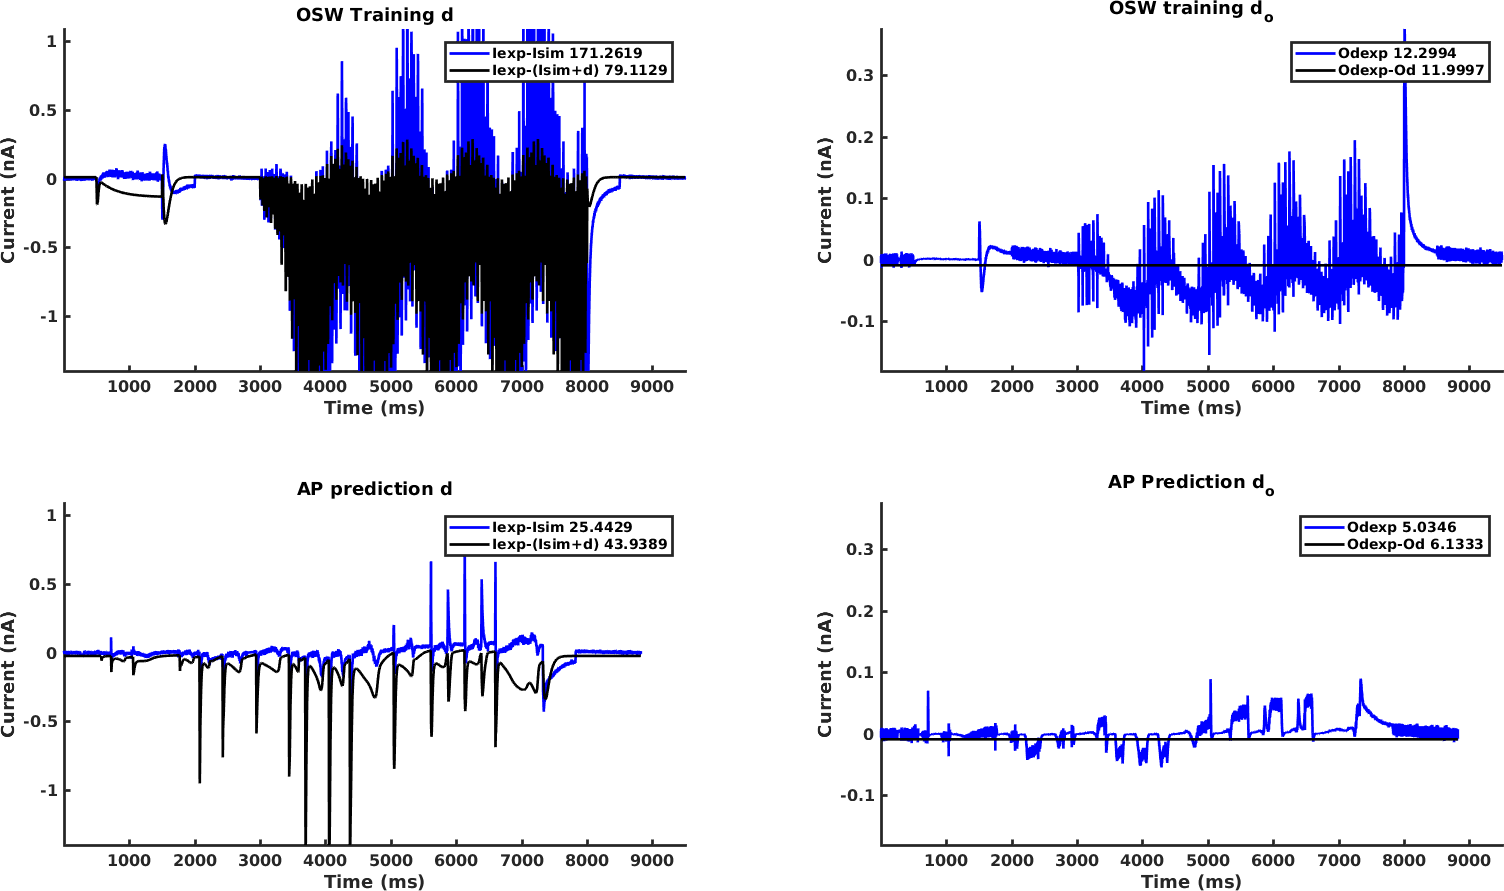
\includegraphics[scale=0.42]{Figures/LASSO_OSW_AP_full_discrepancy.png}
\caption{\textbf{Linear model of discrepancy constructed using LASSO from the OSW protocol.} These models of $d$ (left) and $d_o$ (right) were constructed using LASSO on the entire OSW trace (top), starting with all linearly independent predictors. The root mean square errors between the simulated and predicted traces are shown in the legends. } 
\label{Fig_LASSO_OSW_AP_full_discrepancy}
\end{center}
\end{figure}

\begin{figure}[hb]
\begin{center}
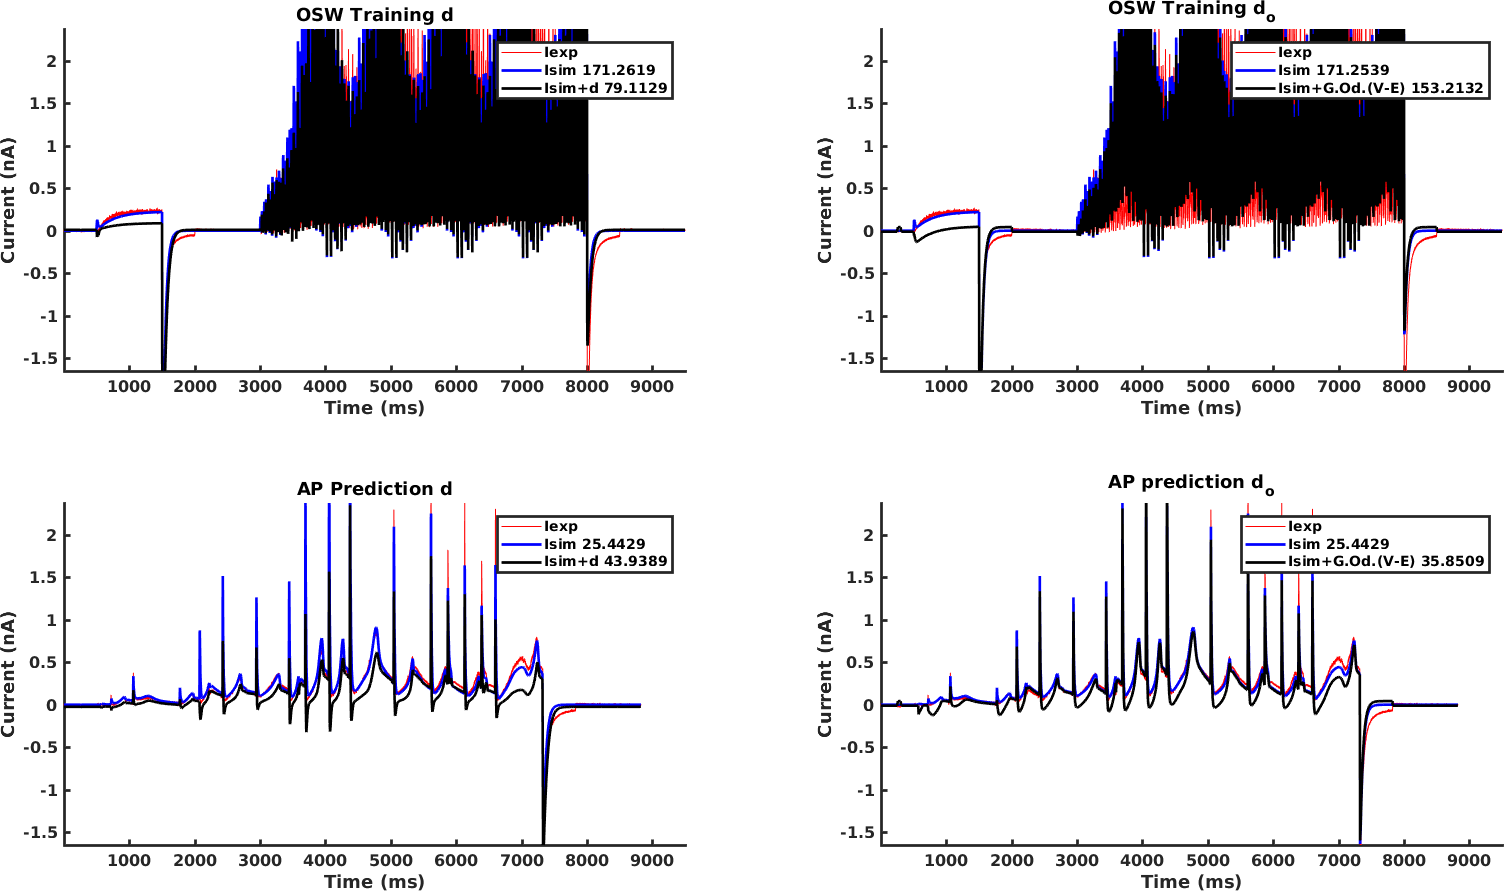
\includegraphics[scale=0.42]{Figures/LASSO_OSW_AP_full_currents.png}
\caption{\textbf{Corrected currents using a linear model of discrepancy constructed using LASSO from the OSW protocol.} The models of $d$ (left) and $d_o$ (right) in Fig. ~\ref{Fig_LASSO_OSW_AP_full_discrepancy} have been incorporated into the simulation (blue line), giving a revised prediction for the OSW and AP protocols (black line). The sum of squared errors between the models and the data are shown in the legend.}
\label{Fig_LASSO_OSW_AP_full_currents}
\end{center}
\end{figure}

\clearpage

\begin{figure}[t]
\begin{center}
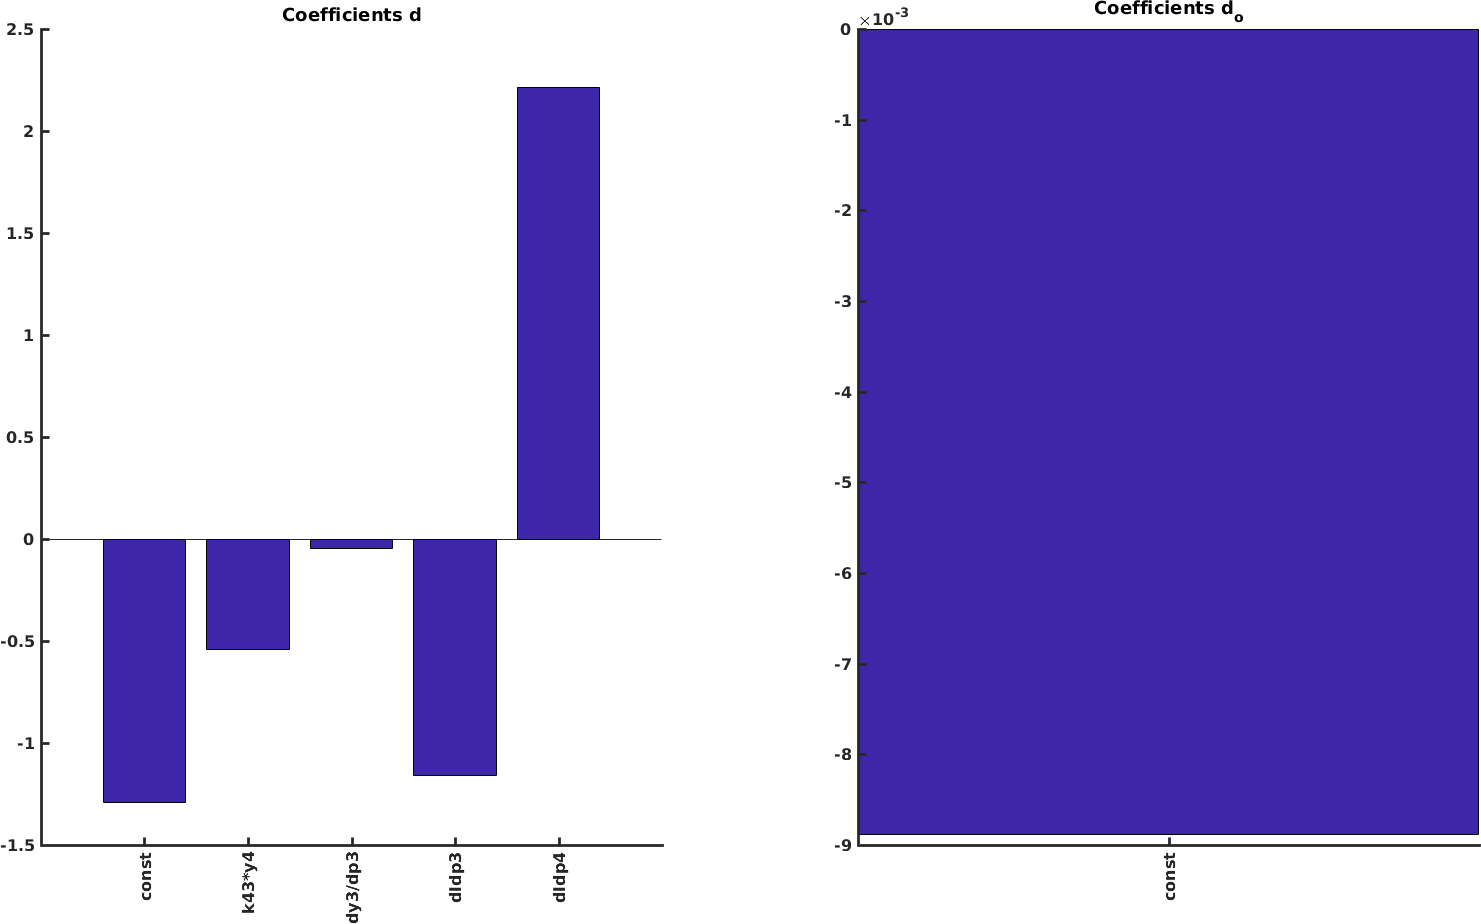
\includegraphics[scale=0.42]{Figures/LASSO_OSW_AP_full_coefficients.png}
\caption{\textbf{Coefficients in the linear model of discrepancy constructed using LASSO from the sine wave generated component of the OSW protocol.} This plot shows the included parameters and coefficients for the model produced by LASSO shown in Fig.~\ref{Fig_LASSO_OSW_AP_full_discrepancy} and Fig.~\ref{Fig_LASSO_OSW_AP_full_currents}. Coefficients for $d$ are shown on the left, and coefficients for $d_o$ are shown on the right.} 
\label{Fig_LASSO_OSW_AP_full_coefficients}
\end{center}
\end{figure}

\begin{figure}[hb]
\begin{center}
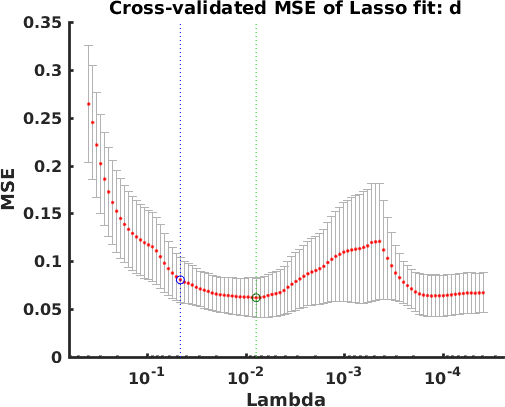
\includegraphics[scale=0.42]{Figures/LASSO_OSW_AP_full_lambda_d.png}
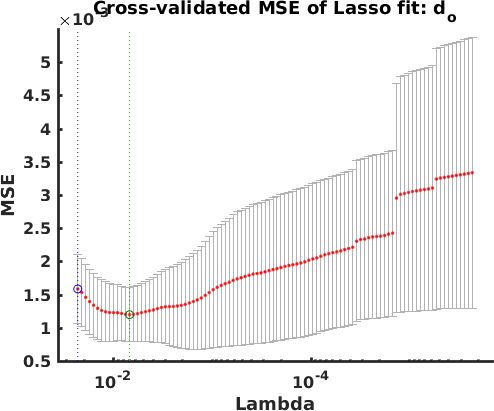
\includegraphics[scale=0.42]{Figures/LASSO_OSW_AP_full_lambda_od.png}
\caption{\textbf{$\lambda$ and Mean Squared Error plots from the linear models of the sine wave component of the OSW protocol.} The models of $d$ (left) and $d_o$ (right) have been generated by varying $\lambda$. The error bars indicate the standard error in the MSE between folds. The value of $\lambda$ giving the minimum MSE is indicated by the green line and the selected value of $\lambda$, being the largest value of $\lambda$ with an MSE within one standard error of the minimum, is shown in blue. Note that $\lambda$ runs from largest to smallest, so that the largest model is on the left.}
\label{Fig_LASSO_OSW_AP_core_lambda}
\end{center}
\end{figure}

\clearpage

\begin{figure}[t]
\begin{center}
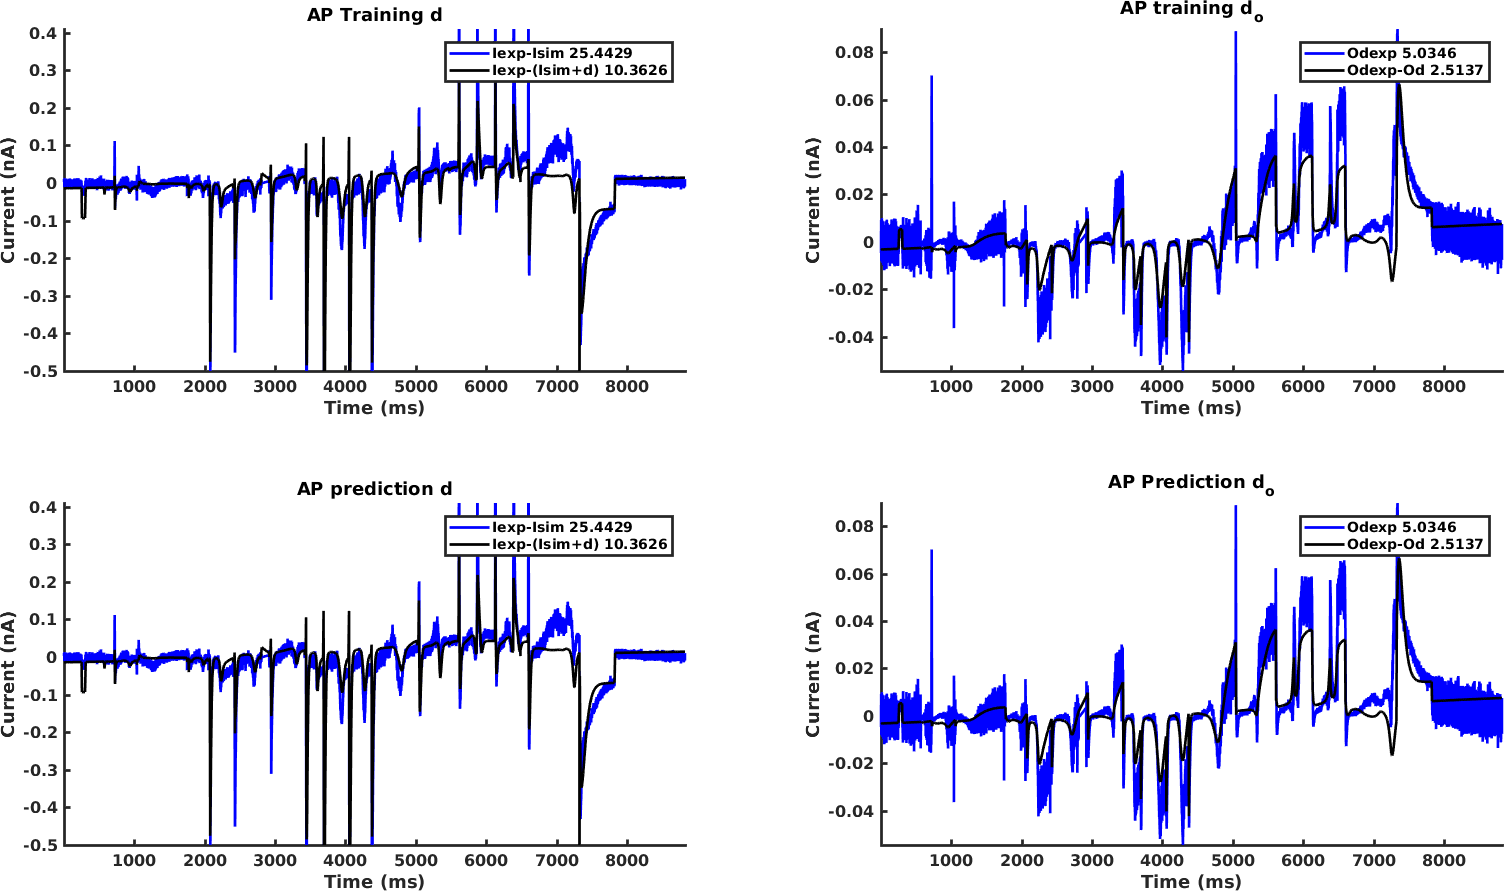
\includegraphics[scale=0.42]{Figures/LASSO_AP_AP_full_discrepancy.png}
\caption{\textbf{Linear model of discrepancy constructed using LASSO from the AP protocol.} These models of $d$ (left) and $d_o$ (right) were constructed using LASSO on the entire AP trace (top), starting with all linearly independent predictors. The root mean square errors between the simulated and predicted traces are shown in the legends. } 
\label{Fig_LASSO_AP_AP_full_discrepancy}
\end{center}
\end{figure}

\begin{figure}[hb]
\begin{center}
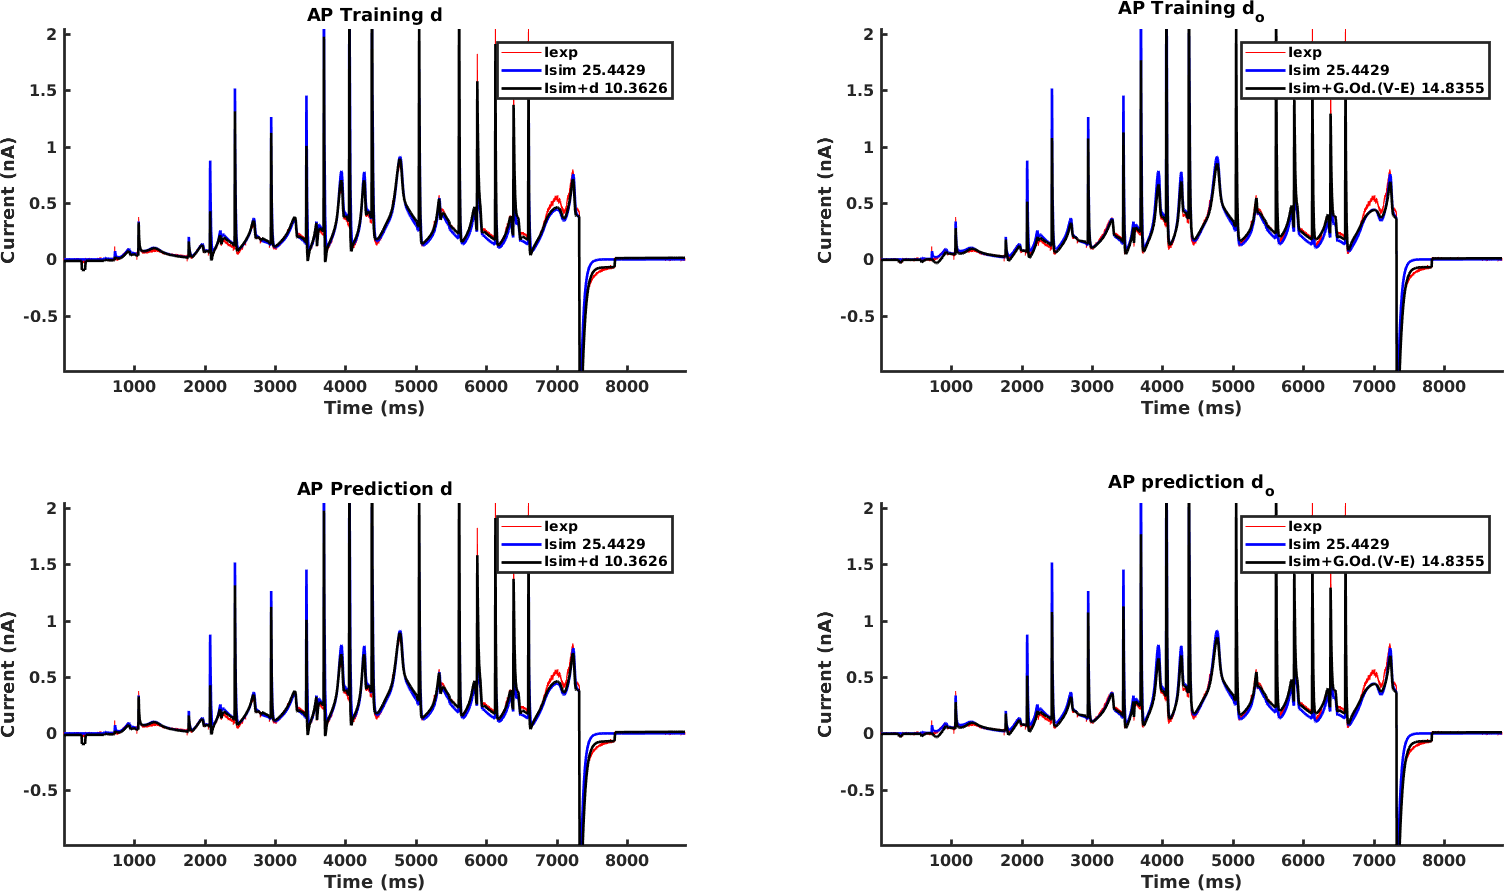
\includegraphics[scale=0.42]{Figures/LASSO_AP_AP_full_currents.png}
\caption{\textbf{Corrected currents using a linear model of discrepancy constructed using LASSO from the AP protocol.} The models of $d$ (left) and $d_o$ (right) in Fig. ~\ref{Fig_LASSO_AP_AP_full_discrepancy} have been incorporated into the simulation (blue line), giving a revised prediction for the AP protocol (black line). The sum of squared errors between the models and the data are shown in the legend.}
\label{Fig_LASSO_AP_AP_full_currents}
\end{center}
\end{figure}

\clearpage

\begin{figure}[t]
\begin{center}
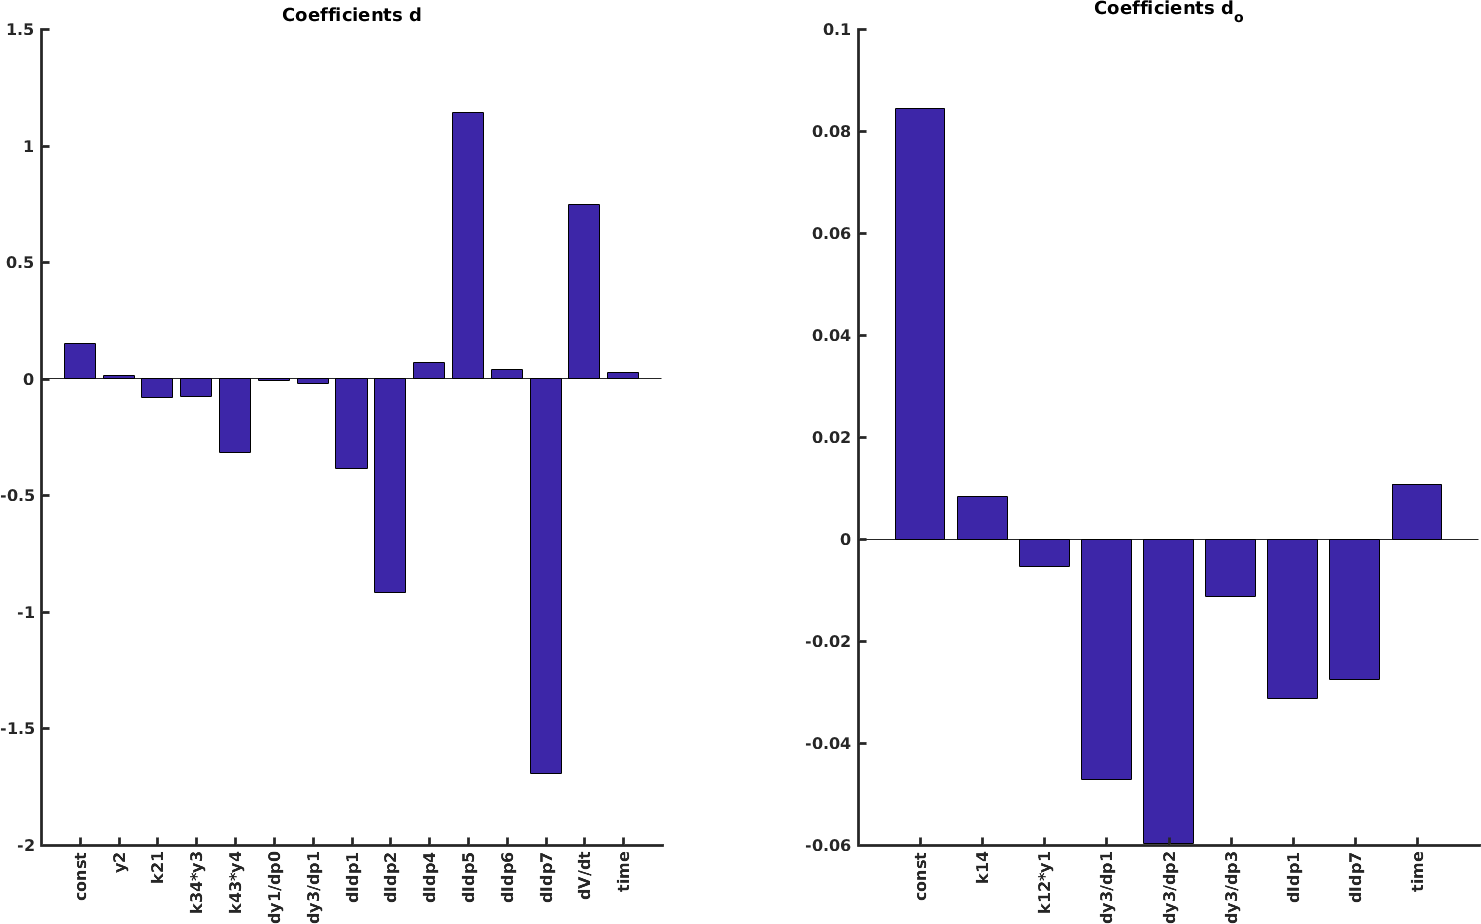
\includegraphics[scale=0.42]{Figures/LASSO_AP_AP_full_coefficients.png}
\caption{\textbf{Coefficients in the linear model of discrepancy constructed using LASSO from the sine wave generated component of the AP protocol.} This plot shows the included parameters and coefficients for the model produced by LASSO shown in Fig.~\ref{Fig_LASSO_AP_AP_full_discrepancy} and Fig.~\ref{Fig_LASSO_AP_AP_full_currents}. Coefficients for $d$ are shown on the left, and coefficients for $d_o$ are shown on the right.} 
\label{Fig_LASSO_AP_AP_full_coefficients}
\end{center}
\end{figure}

\begin{figure}[hb]
\begin{center}
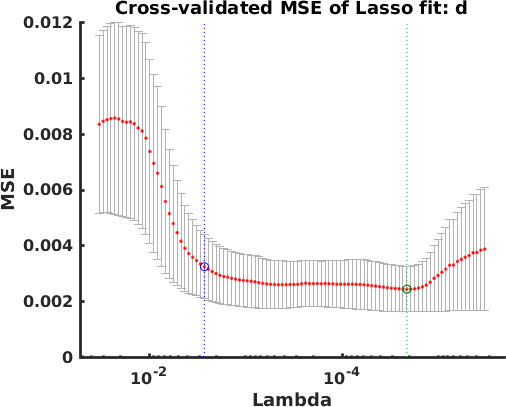
\includegraphics[scale=0.42]{Figures/LASSO_AP_AP_full_lambda_d.png}
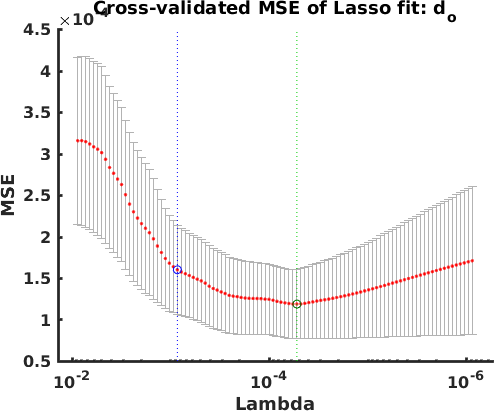
\includegraphics[scale=0.42]{Figures/LASSO_AP_AP_full_lambda_od.png}
\caption{\textbf{$\lambda$ and Mean Squared Error plots from the linear models of the sine wave component of the AP protocol.} The models of $d$ (left) and $d_o$ (right) have been generated by varying $\lambda$. The error bars indicate the standard error in the MSE between folds. The value of $\lambda$ giving the minimum MSE is indicated by the green line and the selected value of $\lambda$, being the largest value of $\lambda$ with an MSE within one standard error of the minimum, is shown in blue. Note that $\lambda$ runs from largest to smallest, so that the largest model is on the left.}
\label{Fig_LASSO_AP_AP_full_lambda}
\end{center}
\end{figure}

\clearpage

\subsection{Predicting Discrepancy Using Stepwise Linear Model}\label{SubSec_StepwiseLM_Discrepancy}
\subsubsection{The Method}
Stepwise Linear Model (StepwiseLM) is a Matlab method for constructing linear models using a stepwise approach\footnote{\url{https://www.mathworks.com/help/stats/stepwiselm.html}}. The method includes predictors in a stepwise manner by first building  up a model by examining all non-included predictors, checking if any have a value below a set entrance tolerance, then including the predictor with the smallest value in the model. Once no more terms can be added to the model, the reverse process is applied and terms are removed from the model if they exceed a removal value. Further terms are then added as before. The final model is then produced when no more predictors can be removed from the model. The method also allows for higher order terms such as interactions and quadratic terms. Initial experiments showed that this approach led to high degrees of overfitting and so was rejected. A number of criteria are available for setting the threshold for including predictors into the model\cite{Wasserman2010}, being
\begin{itemize}
\item $F$-test of the change in the sum of squared error 
\item Aikake Information Criterion (AIC), $\ell_S-|S|$ where $\ell_S$ is the log-likelihood of the model $S$ evaluated at the maximum likelihood estimate, and $|S|$ is the number of predictors in the model.
\item Bayesian Information Criterion (BIC), $\ell_S-\frac{|S|}{2} \log( n )$, where $n$ is the number of data points. BIC penalizes model size more heavily than AIC.
\item Increase in $R^2$
\item Increase in adjusted $R^2$
\end{itemize}
For the plots in Section \ref{SubSubSec_StepwiseLM_Results}, we used AIC with the Matlab default values for entering ($0$) and removal from ($0.1$) the model. The choice of AIC was motivated by the poor performance of the smaller models produced by LASSO, which made BIC a less attractive criterion.

The StepwiseLM method has the appealing feature that it can include polynomial interaction terms to arbitrary order, for example interactions ($X_iX_j$) or quadratic terms ($X_i^2$). Preliminary experiments found that these methods resulted in an enormous degree of over-fitting and very poor prediction. Consequently, they have been omitted from this report.

\subsubsection{Results}\label{SubSubSec_StepwiseLM_Results}
This section shows the same data as for the LASSO results shown above in Section \ref{SubSec_Lasso_Discrepancy}. Because stepwiselm does not use regularization, no lambda plots are shown. In general, the model tended to over-fit, rather than under-fit as for LASSO. As a result, the general trend is for a reasonable fit to the training data but a poor fit during prediction.

\begin{figure}[t]
\begin{center}
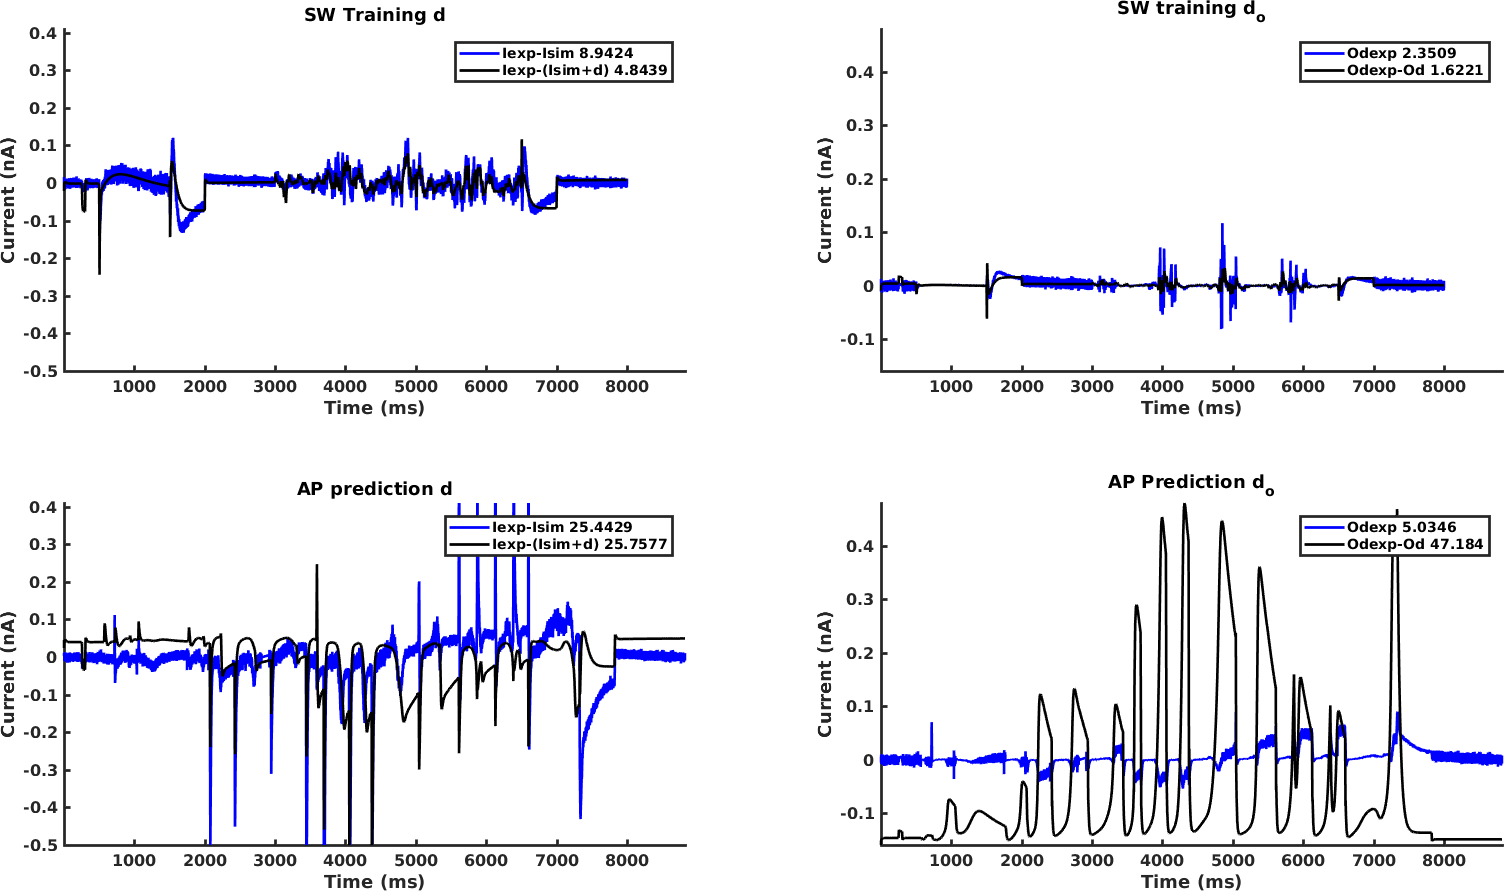
\includegraphics[scale=0.42]{Figures/StepwiseLM_SW_AP_full_discrepancy.png}
\caption{\textbf{Linear model of discrepancy constructed using StepwiseLM from the SW protocol.} These models of $d$ (left) and $d_o$ (right) were constructed using StepwiseLM on the entire SW trace (top), starting with all linearly independent predictors. The improvement of the training trace (top) is poor and the resulting models fail to predict the discrepancy in the AP trace (bottom). The root mean square errors between the simulated and predicted traces are shown in the legends. } 
\label{Fig_StepwiseLM_SW_AP_full_discrepancy}
\end{center}
\end{figure}

\begin{figure}[hb]
\begin{center}
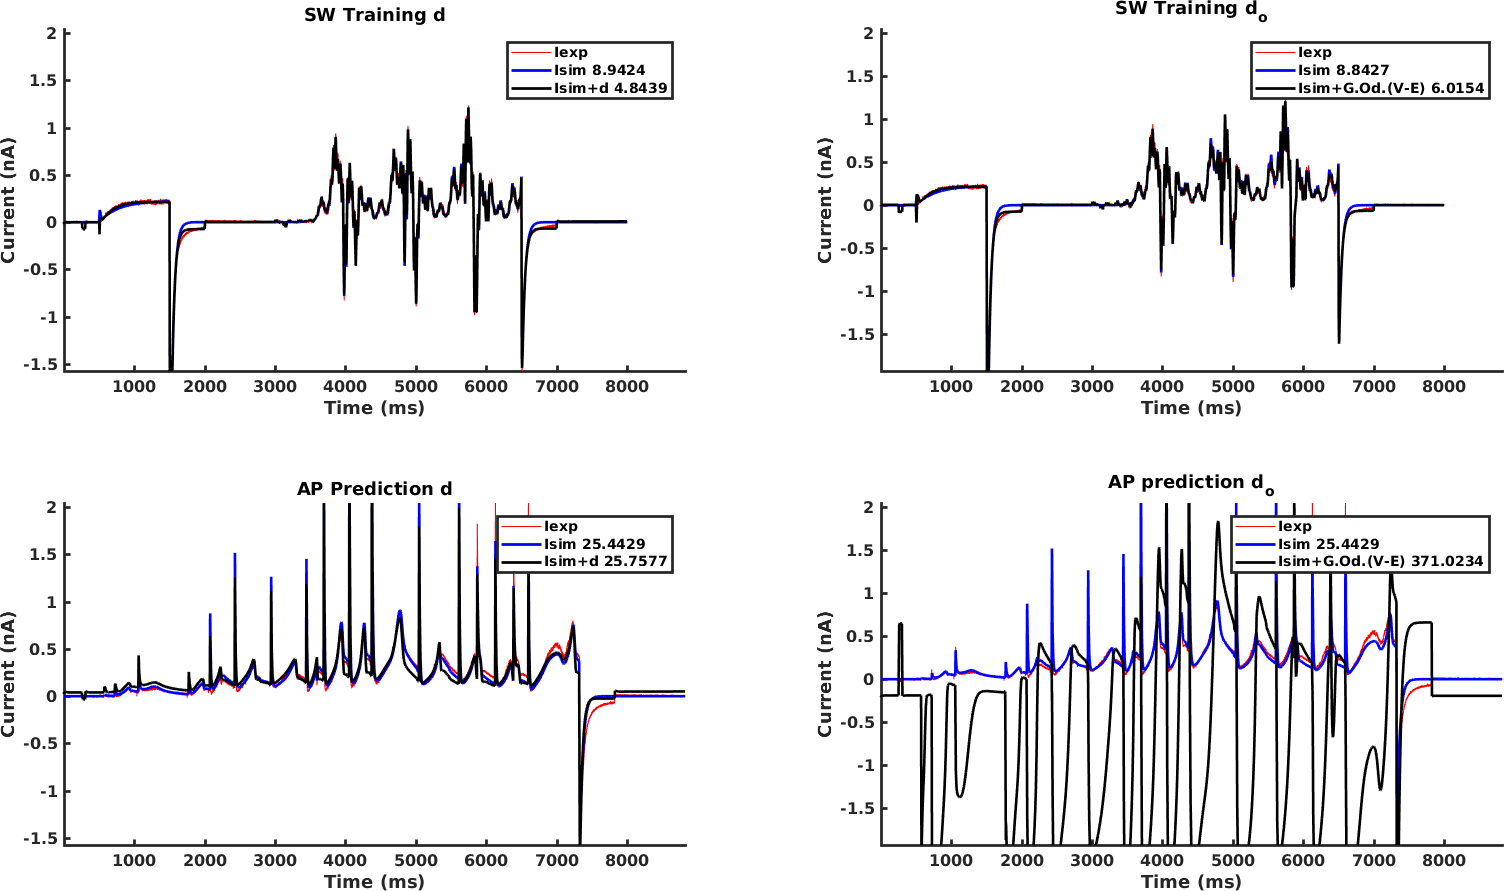
\includegraphics[scale=0.42]{Figures/StepwiseLM_SW_AP_full_currents.png}
\caption{\textbf{Corrected currents using a linear model of discrepancy constructed using StepwiseLM from the SW protocol.} The models of $d$ (left) and $d_o$ (right) in Fig. ~\ref{Fig_StepwiseLM_SW_AP_full_discrepancy} have been incorporated into the simulation (blue line), giving a revised prediction for the SW and AP protocols (black line). As expected from Fig.~\ref{Fig_StepwiseLM_SW_AP_full_discrepancy}, there is little improvement in the agreement with the experimental data (red line). The sum of squared errors between the models and the data are shown in the legend.}
\label{Fig_StepwiseLM_SW_AP_full_currents}
\end{center}
\end{figure}

\begin{figure}[t]
\begin{center}
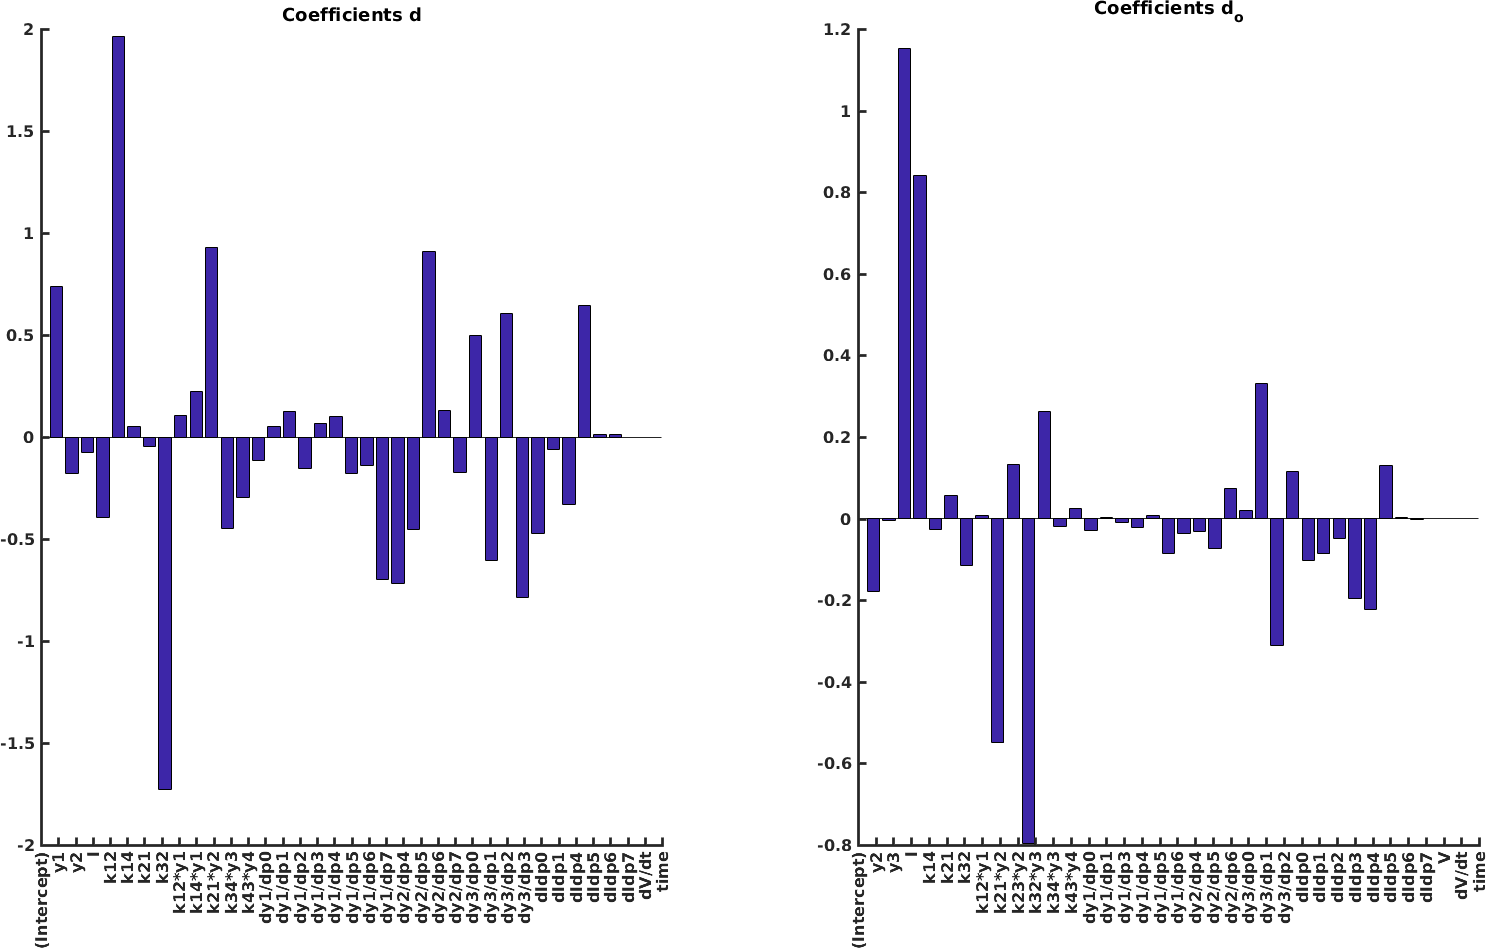
\includegraphics[scale=0.42]{Figures/StepwiseLM_SW_AP_full_coefficients.png}
\caption{\textbf{Coefficients in the linear model of discrepancy constructed using StepwiseLM from the SW protocol.} This plot shows the included parameters and coefficients for the model produced by StepwiseLM shown in Fig.~\ref{Fig_StepwiseLM_SW_AP_full_discrepancy} and Fig.~\ref{Fig_StepwiseLM_SW_AP_full_currents}. Coefficients for $d$ are shown on the left, and coefficients for $d_o$ are shown on the right.} 
\label{Fig_StepwiseLM_SW_AP_coefficients}
\end{center}
\end{figure}

\clearpage

\begin{figure}[t]
\begin{center}
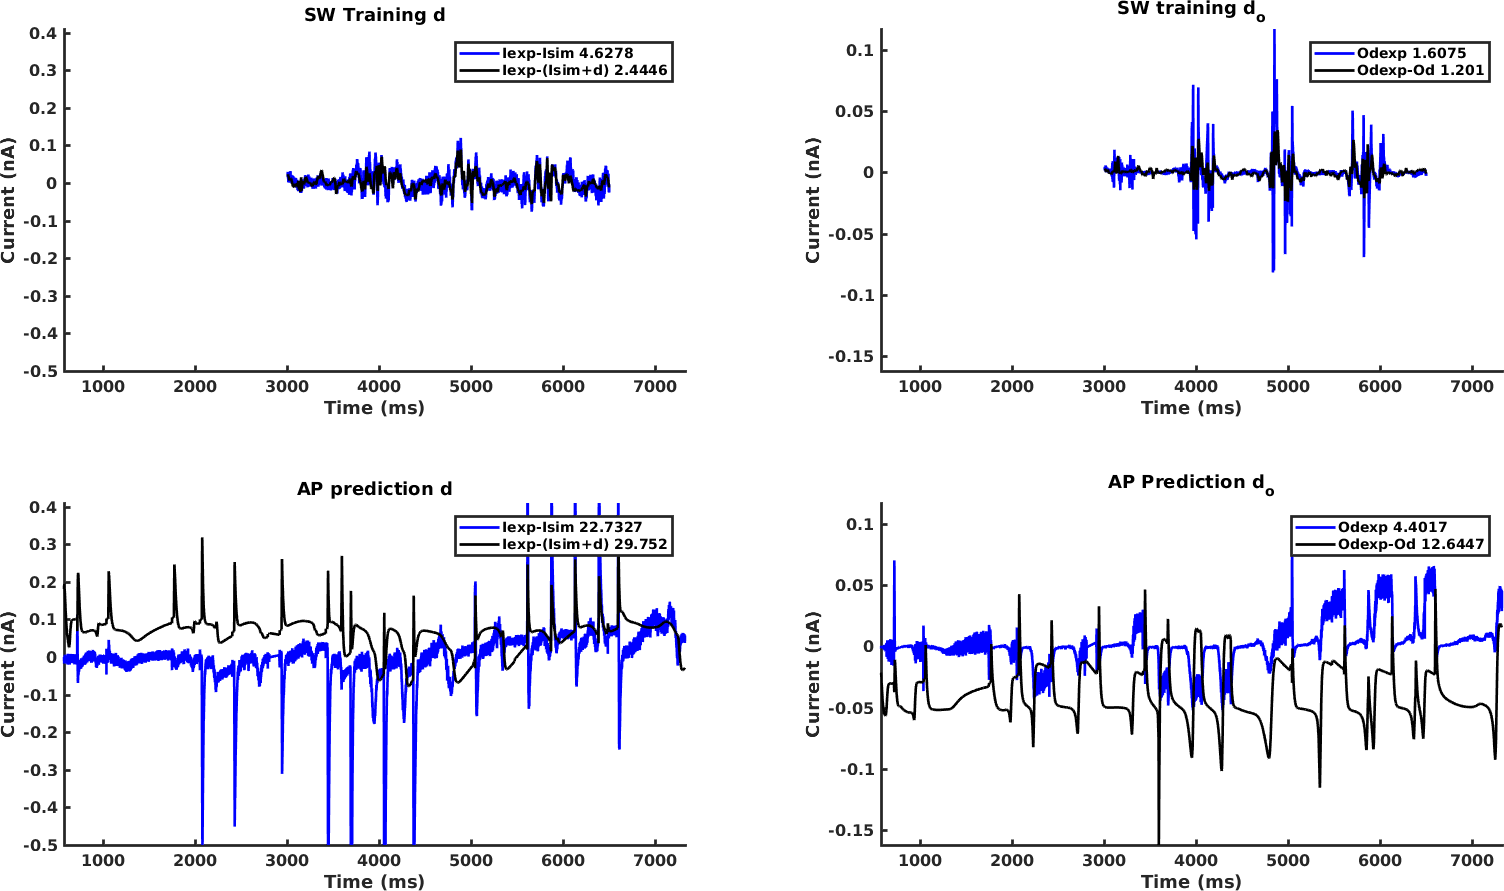
\includegraphics[scale=0.42]{Figures/StepwiseLM_SW_AP_core_discrepancy.png}
\caption{\textbf{Linear model of discrepancy constructed using StepwiseLM.} These models of $d$ (left) and $d_o$ (right) were constructed using StepwiseLM on the entire SW trace (top), starting with all linearly independent predictors. The root mean square errors between the simulated and predicted traces are shown in the legends. } 
\label{Fig_StepwiseLM_SW_AP_core_discrepancy}
\end{center}
\end{figure}

\begin{figure}[hb]
\begin{center}
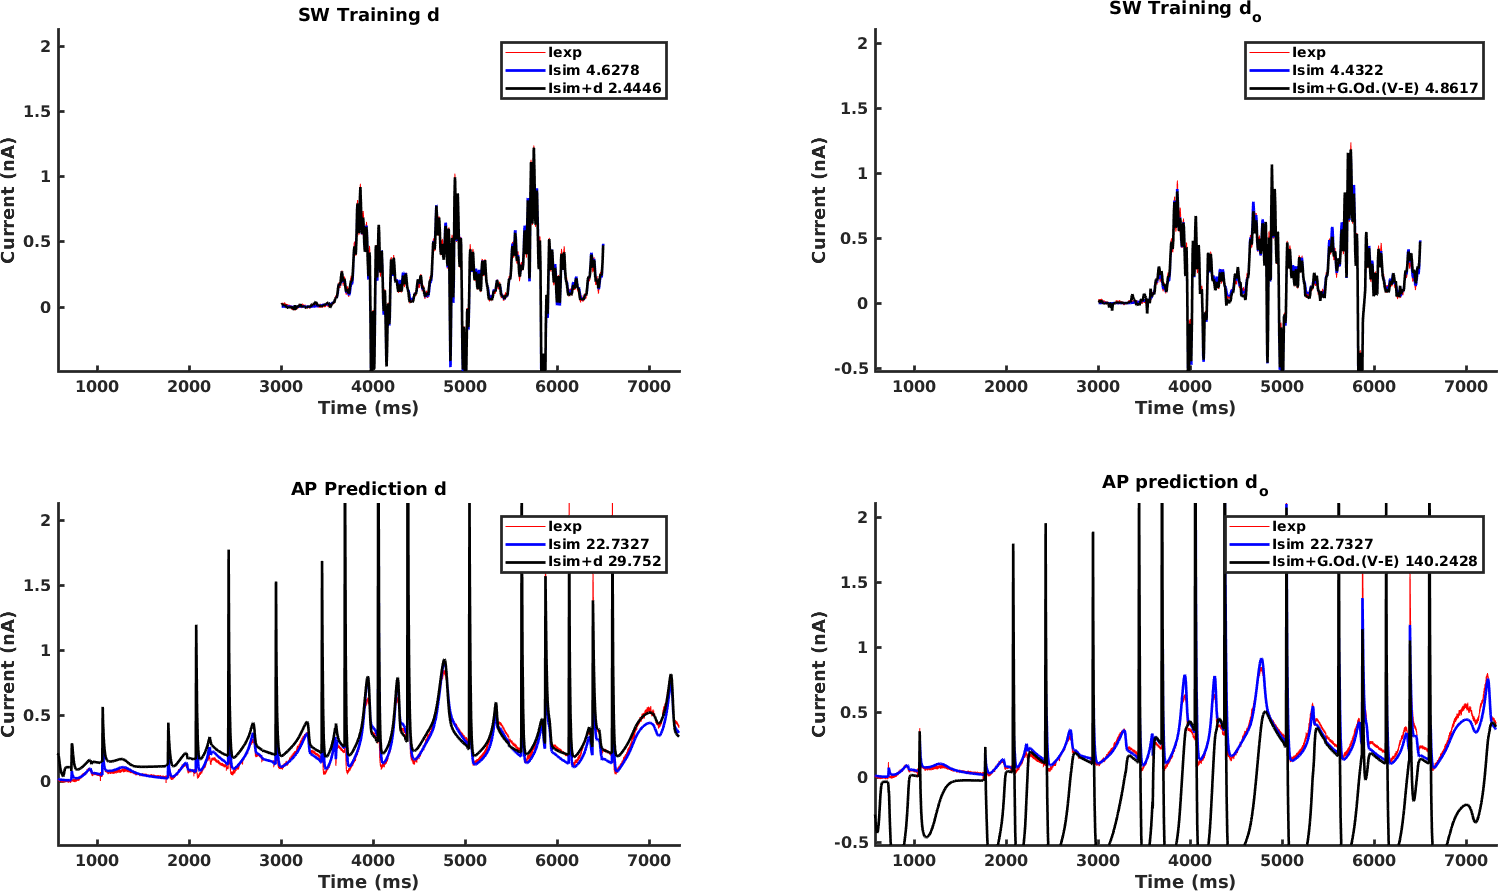
\includegraphics[scale=0.42]{Figures/StepwiseLM_SW_AP_core_currents.png}
\caption{\textbf{Corrected currents using a linear model of discrepancy constructed using StepwiseLM from the sine wave generated component of the SW protocol.} The models of $d$ (left) and $d_o$ (right) in Fig.~\ref{Fig_StepwiseLM_SW_AP_core_discrepancy} have been incorporated into the simulation (blue line), giving a revised prediction for the SW and AP protocols (black line). The sum of squared errors between the models and the data are shown in the legend.}
\label{Fig_StepwiseLM_SW_AP_core_currents}
\end{center}
\end{figure}

\clearpage

\begin{figure}[t]
\begin{center}
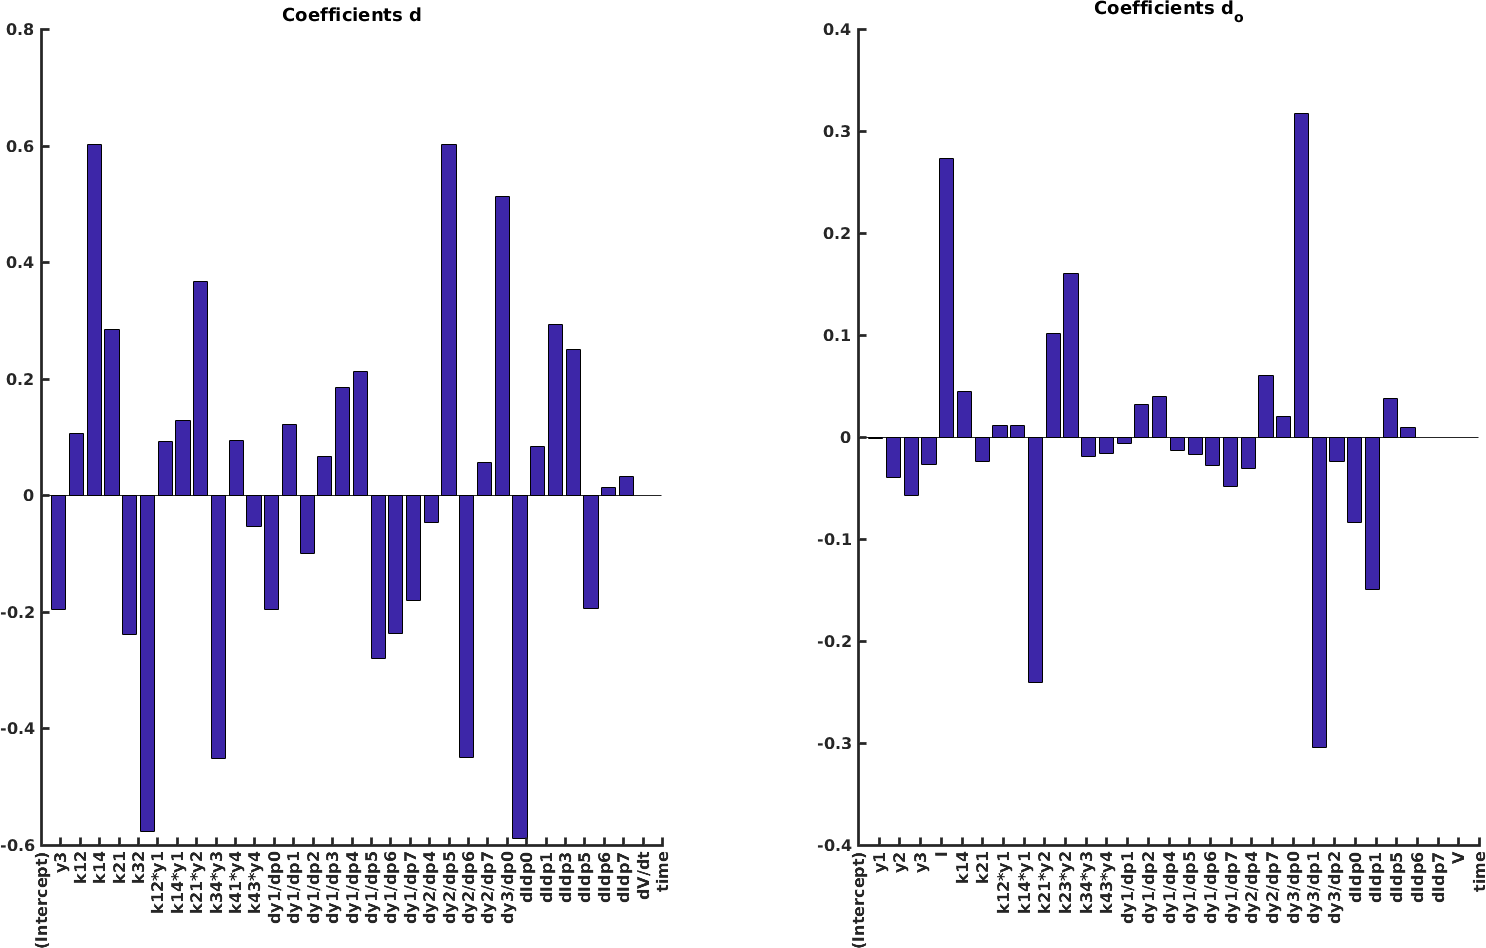
\includegraphics[scale=0.42]{Figures/StepwiseLM_SW_AP_core_coefficients.png}
\caption{\textbf{Coefficients in the linear model of discrepancy constructed using StepwiseLM from the sine wave generated component of the SW protocol.} This plot shows the included parameters and coefficients for the model produced by StepwiseLM shown in Fig.~\ref{Fig_StepwiseLM_SW_AP_core_discrepancy} and Fig.~\ref{Fig_StepwiseLM_SW_AP_core_currents}. Coefficients for $d$ are shown on the left, and coefficients for $d_o$ are shown on the right.} 
\label{Fig_StepwiseLM_SW_AP_core_coefficients}
\end{center}
\end{figure}

\clearpage

\begin{figure}[t]
\begin{center}
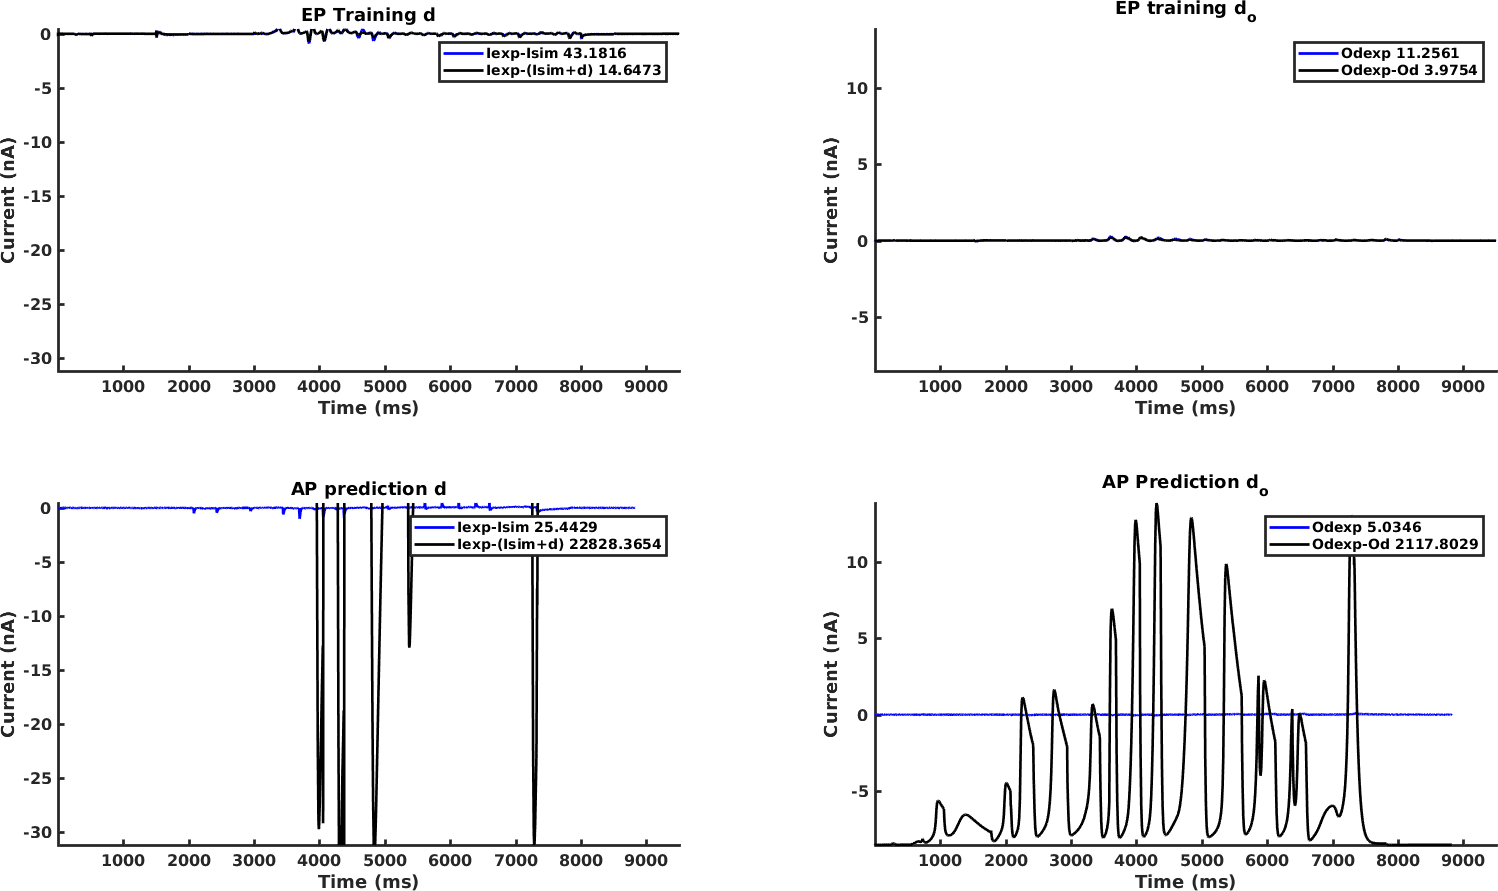
\includegraphics[scale=0.42]{Figures/StepwiseLM_EP_AP_full_discrepancy.png}
\caption{\textbf{Linear model of discrepancy constructed using StepwiseLM from the EP protocol.} These models of $d$ (left) and $d_o$ (right) were constructed using StepwiseLM on the entire SW trace (top), starting with all linearly independent predictors. The root mean square errors between the simulated and predicted traces are shown in the legends. } 
\label{Fig_StepwiseLM_EP_AP_full_discrepancy}
\end{center}
\end{figure}

\begin{figure}[hb]
\begin{center}
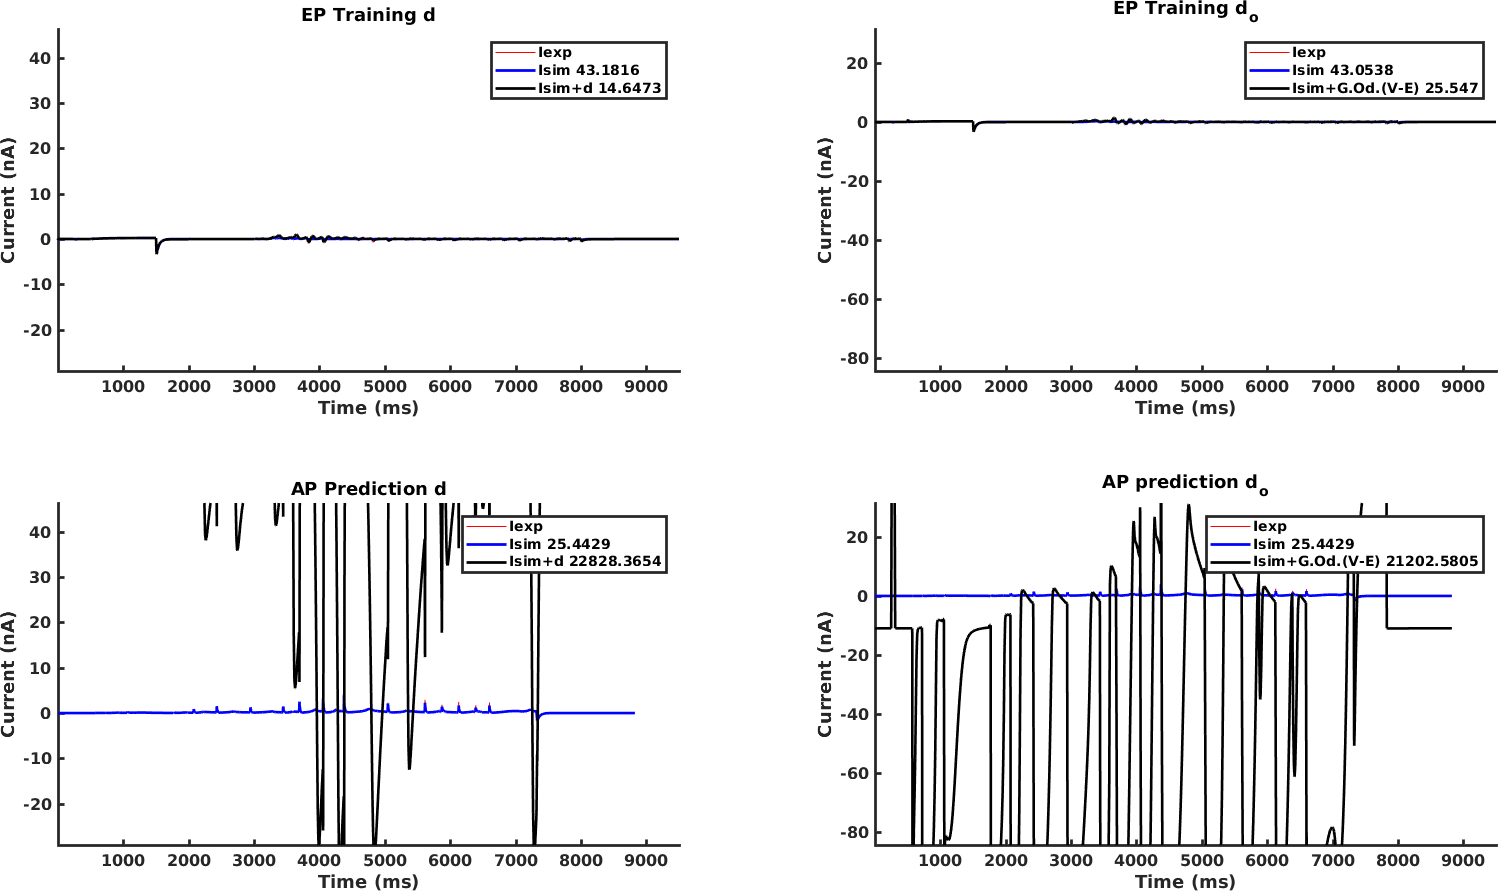
\includegraphics[scale=0.42]{Figures/StepwiseLM_EP_AP_full_currents.png}
\caption{\textbf{Corrected currents using a linear model of discrepancy constructed using StepwiseLM from the EP protocol.} The models of $d$ (left) and $d_o$ (right) in Fig. ~\ref{Fig_StepwiseLM_SW_AP_full_discrepancy} have been incorporated into the simulation (blue line), giving a revised prediction for the EP and AP protocols (black line). The sum of squared errors between the models and the data are shown in the legend.}
\label{Fig_StepwiseLM_EP_AP_full_currents}
\end{center}
\end{figure}

\clearpage

\begin{figure}[t]
\begin{center}
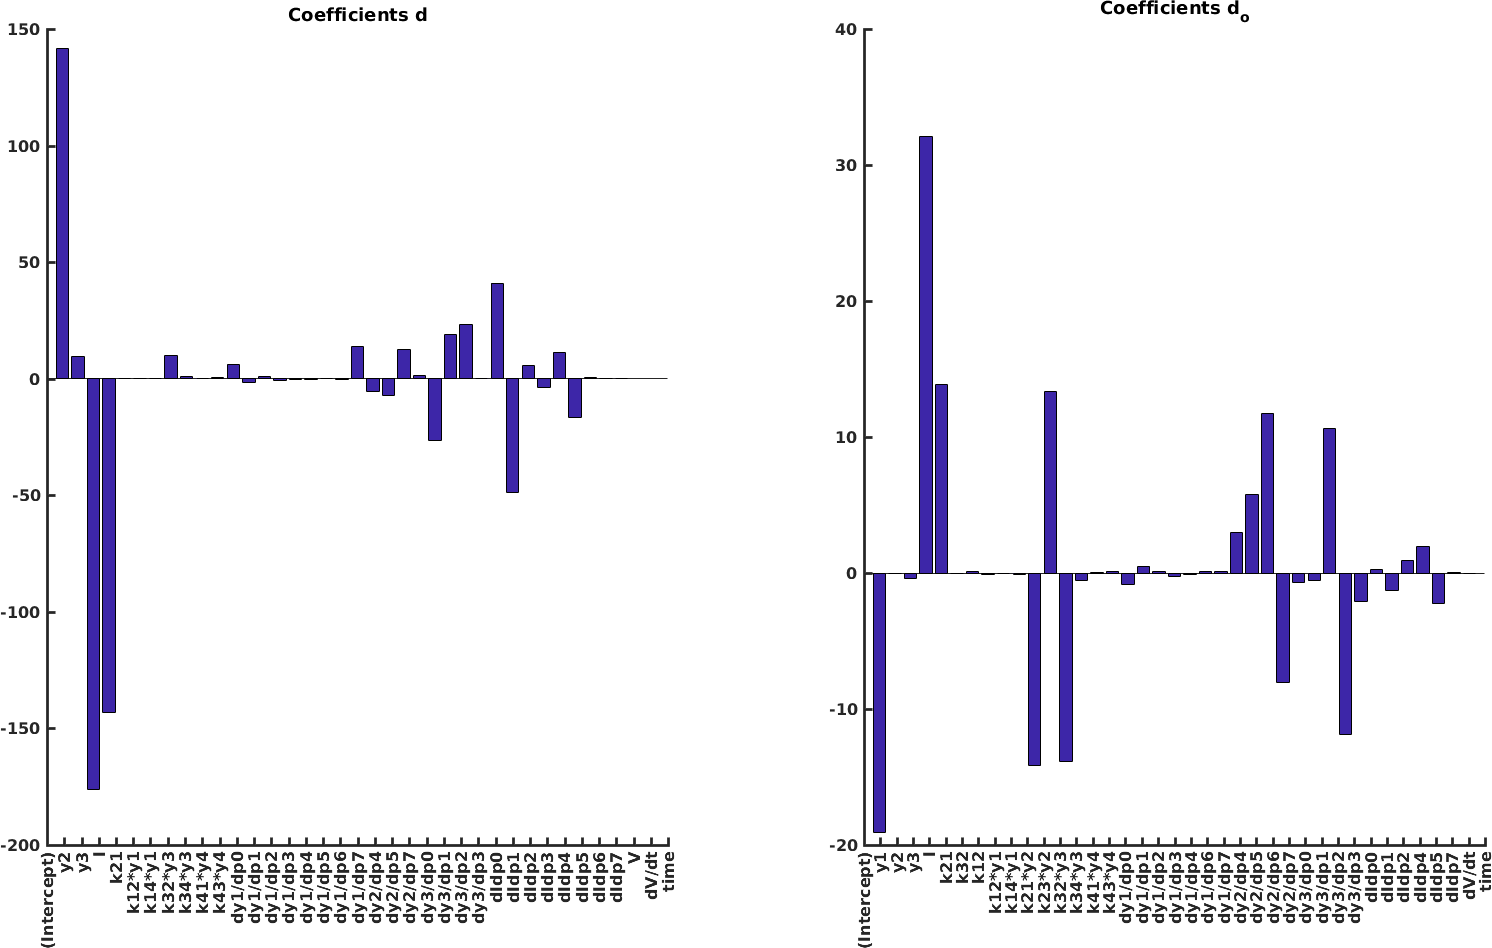
\includegraphics[scale=0.42]{Figures/StepwiseLM_EP_AP_full_coefficients.png}
\caption{\textbf{Coefficients in the linear model of discrepancy constructed using StepwiseLM from the EP protocol.} This plot shows the included parameters and coefficients for the model produced by StepwiseLM shown in Fig.~\ref{Fig_StepwiseLM_EP_AP_full_discrepancy} and Fig.~\ref{Fig_StepwiseLM_EP_AP_full_currents}. Coefficients for $d$ are shown on the left, and coefficients for $d_o$ are shown on the right.} 
\label{Fig_StepwiseLM_EP_AP_full_coefficients}
\end{center}
\end{figure}

\clearpage

\begin{figure}[t]
\begin{center}
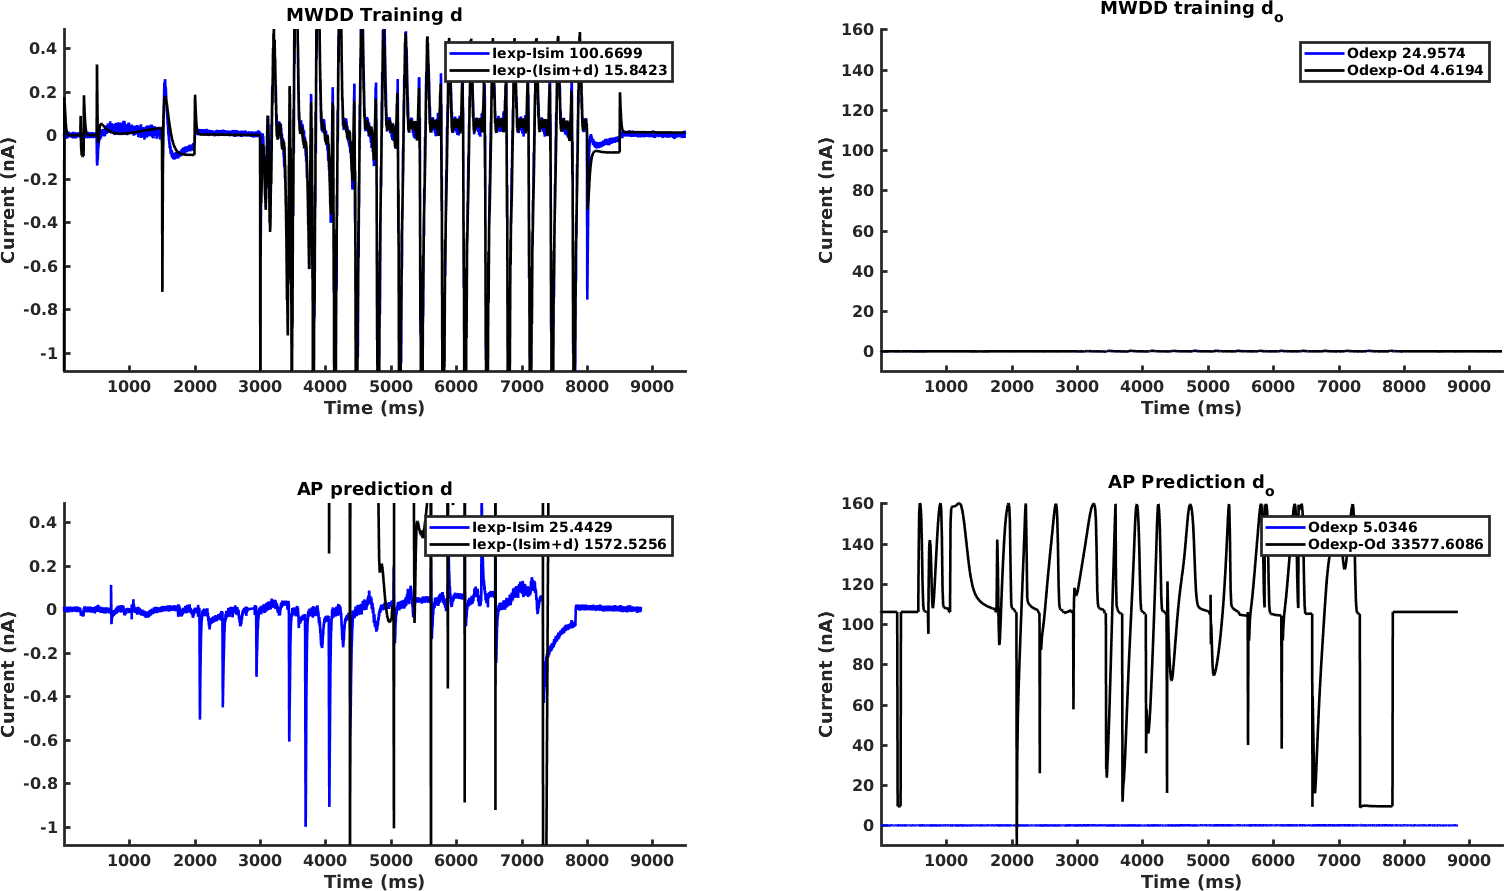
\includegraphics[scale=0.42]{Figures/StepwiseLM_MWDD_AP_full_discrepancy.png}
\caption{\textbf{Linear model of discrepancy constructed using StepwiseLM from the MWDD protocol.} These models of $d$ (left) and $d_o$ (right) were constructed using StepwiseLM on the entire MWDD trace (top), starting with all linearly independent predictors. The root mean square errors between the simulated and predicted traces are shown in the legends. } 
\label{Fig_StepwiseLM_MWDD_AP_full_discrepancy}
\end{center}
\end{figure}

\begin{figure}[hb]
\begin{center}
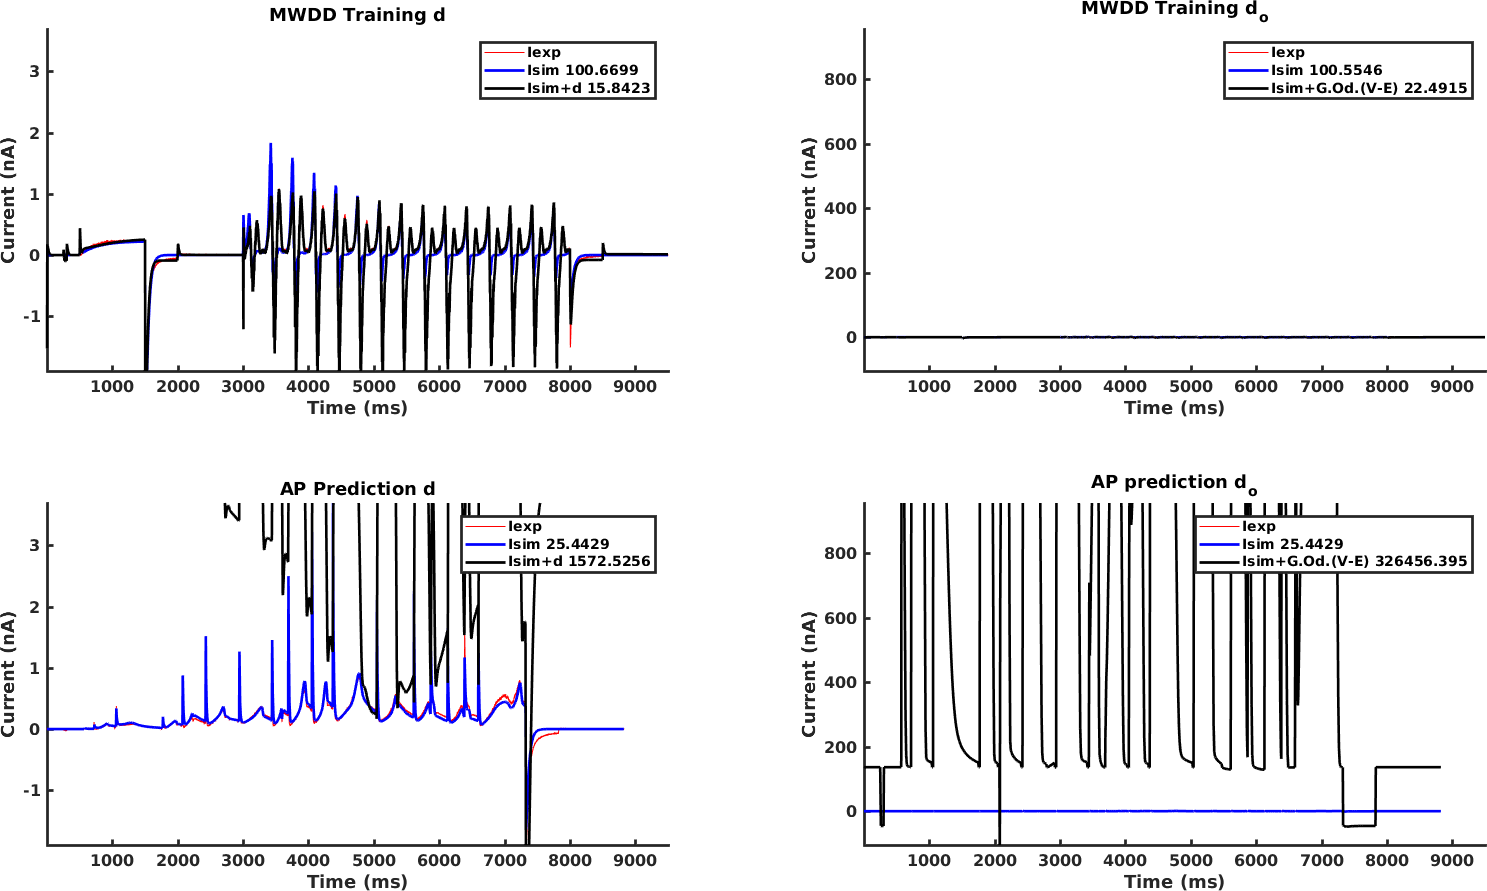
\includegraphics[scale=0.42]{Figures/StepwiseLM_MWDD_AP_full_currents.png}
\caption{\textbf{Corrected currents using a linear model of discrepancy constructed using StepwiseLM from the MWDD protocol.} The models of $d$ (left) and $d_o$ (right) in Fig. ~\ref{Fig_StepwiseLM_MWDD_AP_full_discrepancy} have been incorporated into the simulation (blue line), giving a revised prediction for the MWDD and AP protocols (black line). The sum of squared errors between the models and the data are shown in the legend.}
\label{Fig_StepwiseLM_MWDD_AP_full_currents}
\end{center}
\end{figure}

\clearpage

\begin{figure}[t]
\begin{center}
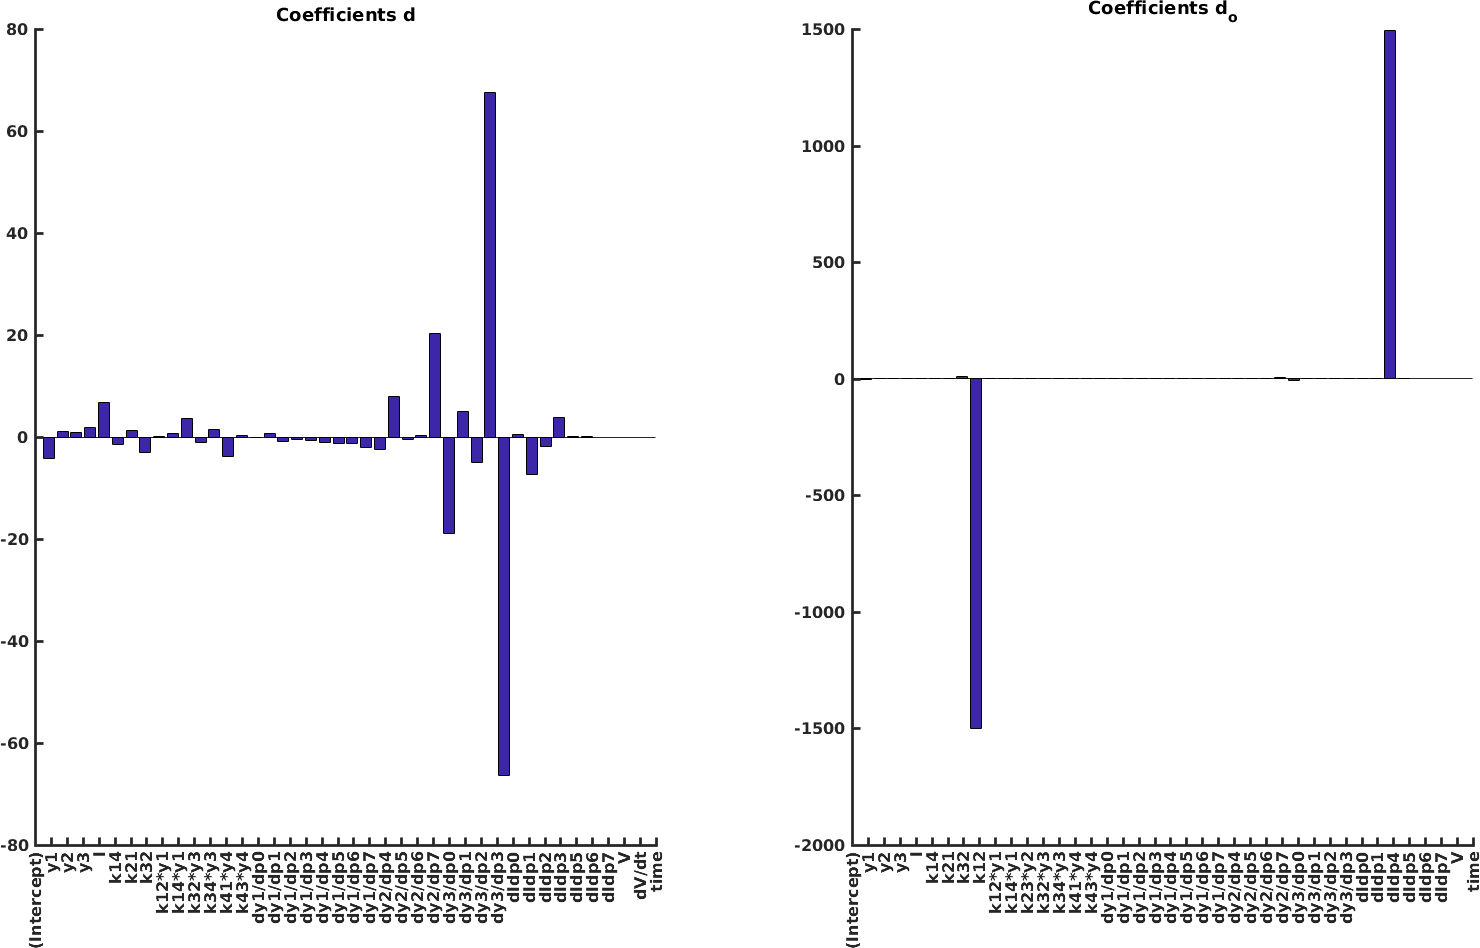
\includegraphics[scale=0.42]{Figures/StepwiseLM_MWDD_AP_full_coefficients.png}
\caption{\textbf{Coefficients in the linear model of discrepancy constructed using StepwiseLM from the MWDD protocol.} This plot shows the included parameters and coefficients for the model produced by StepwiseLM shown in Fig.~\ref{Fig_StepwiseLM_MWDD_AP_full_discrepancy} and Fig.~\ref{Fig_StepwiseLM_MWDD_AP_full_currents}. Coefficients for $d$ are shown on the left, and coefficients for $d_o$ are shown on the right.} 
\label{Fig_StepwiseLM_MWDD_AP_full_coefficients}
\end{center}
\end{figure}

\clearpage

\begin{figure}[t]
\begin{center}
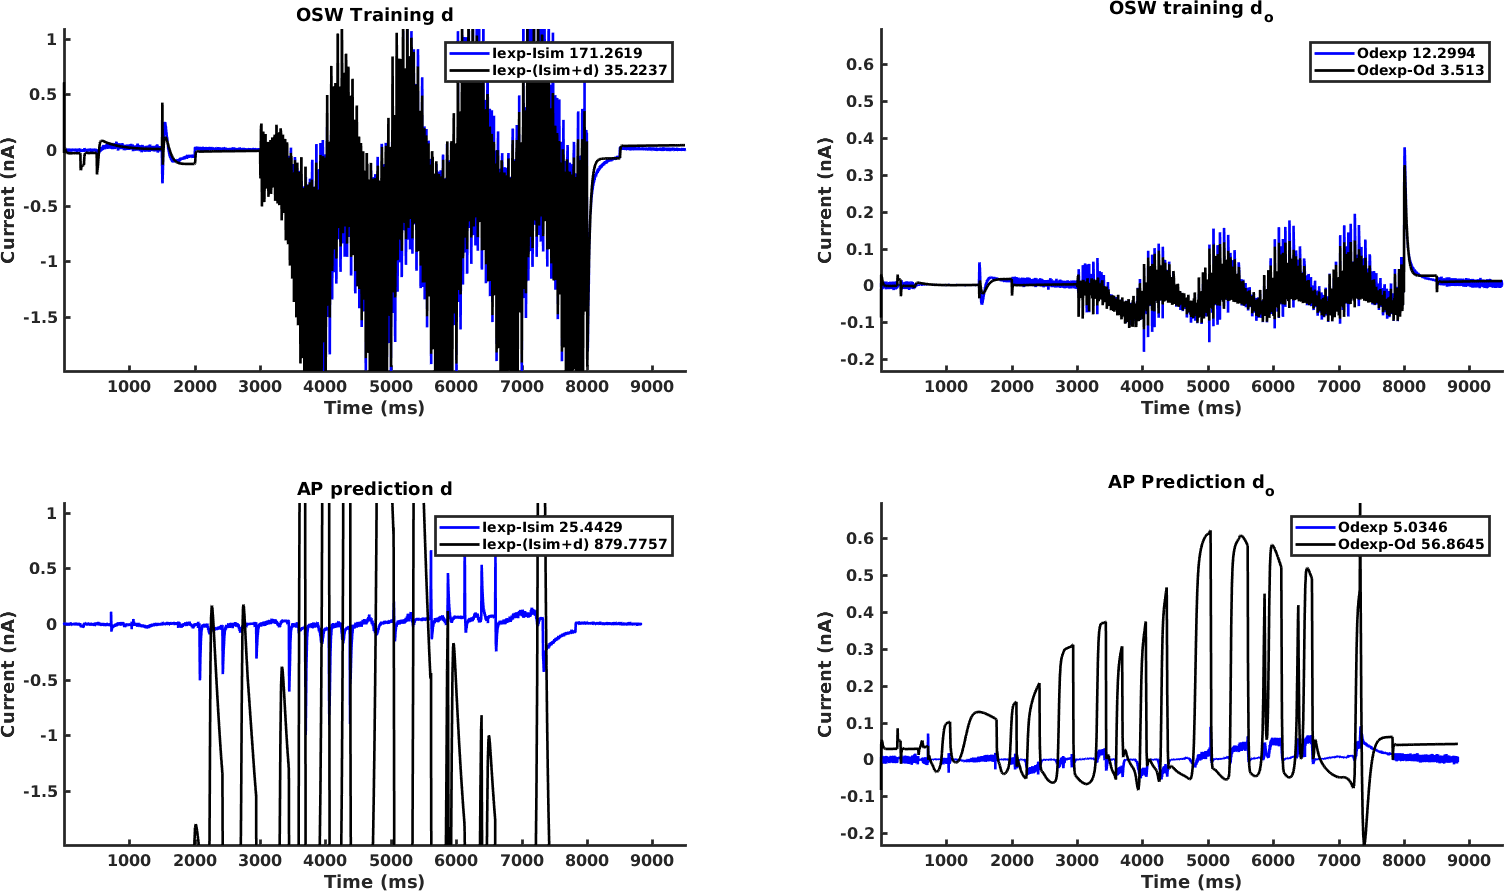
\includegraphics[scale=0.42]{Figures/StepwiseLM_OSW_AP_full_discrepancy.png}
\caption{\textbf{Linear model of discrepancy constructed using StepwiseLM from the OSW protocol.} These models of $d$ (left) and $d_o$ (right) were constructed using StepwiseLM on the entire OSW trace (top), starting with all linearly independent predictors. The root mean square errors between the simulated and predicted traces are shown in the legends. } 
\label{Fig_StepwiseLM_OSW_AP_full_discrepancy}
\end{center}
\end{figure}

\begin{figure}[hb]
\begin{center}
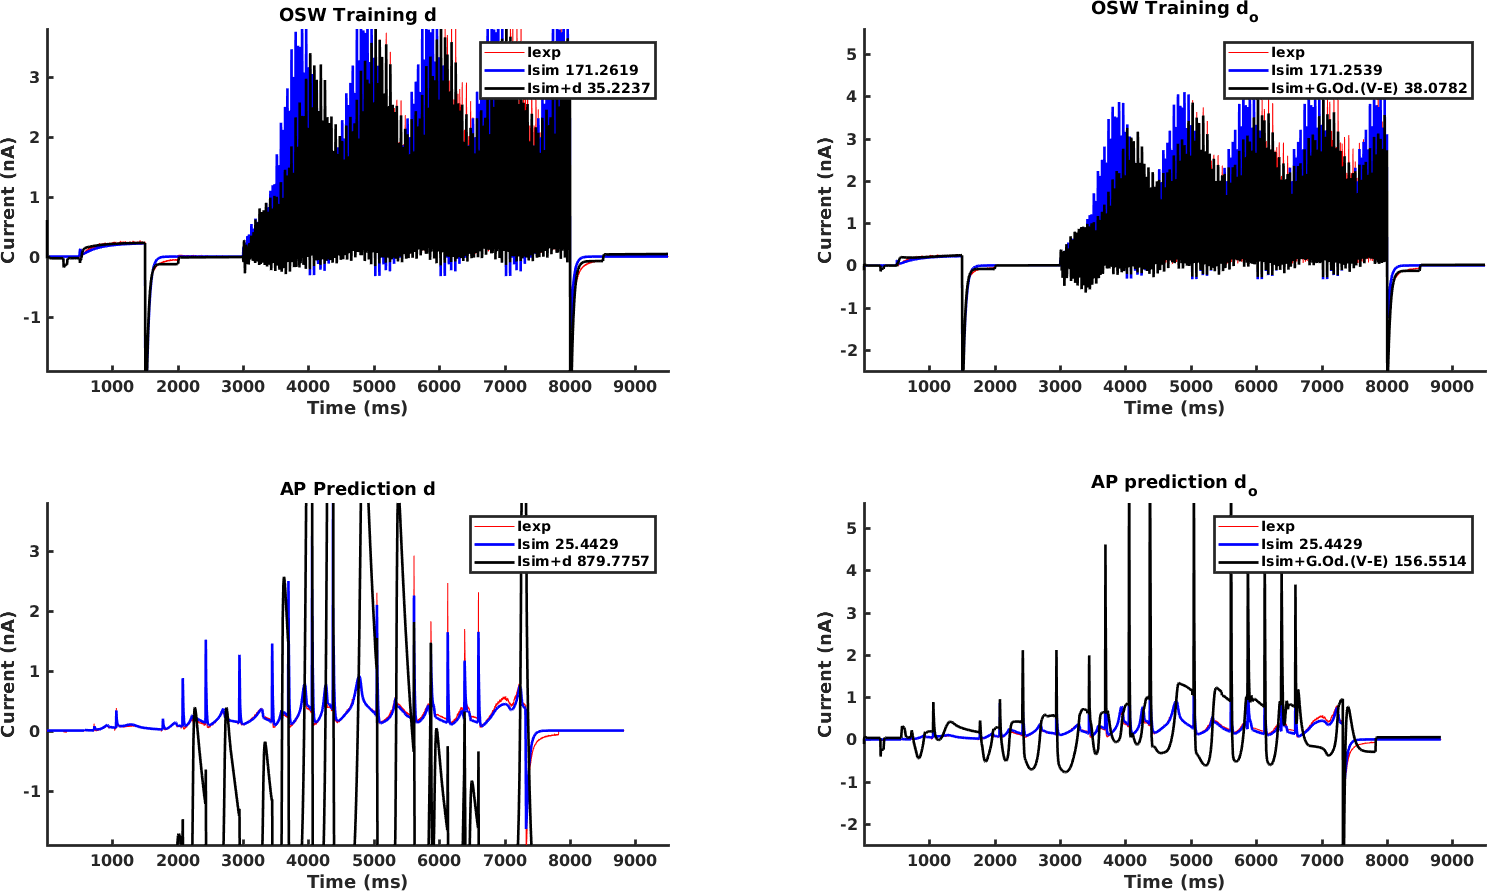
\includegraphics[scale=0.42]{Figures/StepwiseLM_OSW_AP_full_currents.png}
\caption{\textbf{Corrected currents using a linear model of discrepancy constructed using StepwiseLM from the OSW protocol.} The models of $d$ (left) and $d_o$ (right) in Fig. ~\ref{Fig_StepwiseLM_OSW_AP_full_discrepancy} have been incorporated into the simulation (blue line), giving a revised prediction for the OSW and AP protocols (black line). The sum of squared errors between the models and the data are shown in the legend.}
\label{Fig_StepwiseLM_OSW_AP_full_currents}
\end{center}
\end{figure}

\clearpage

\begin{figure}[t]
\begin{center}
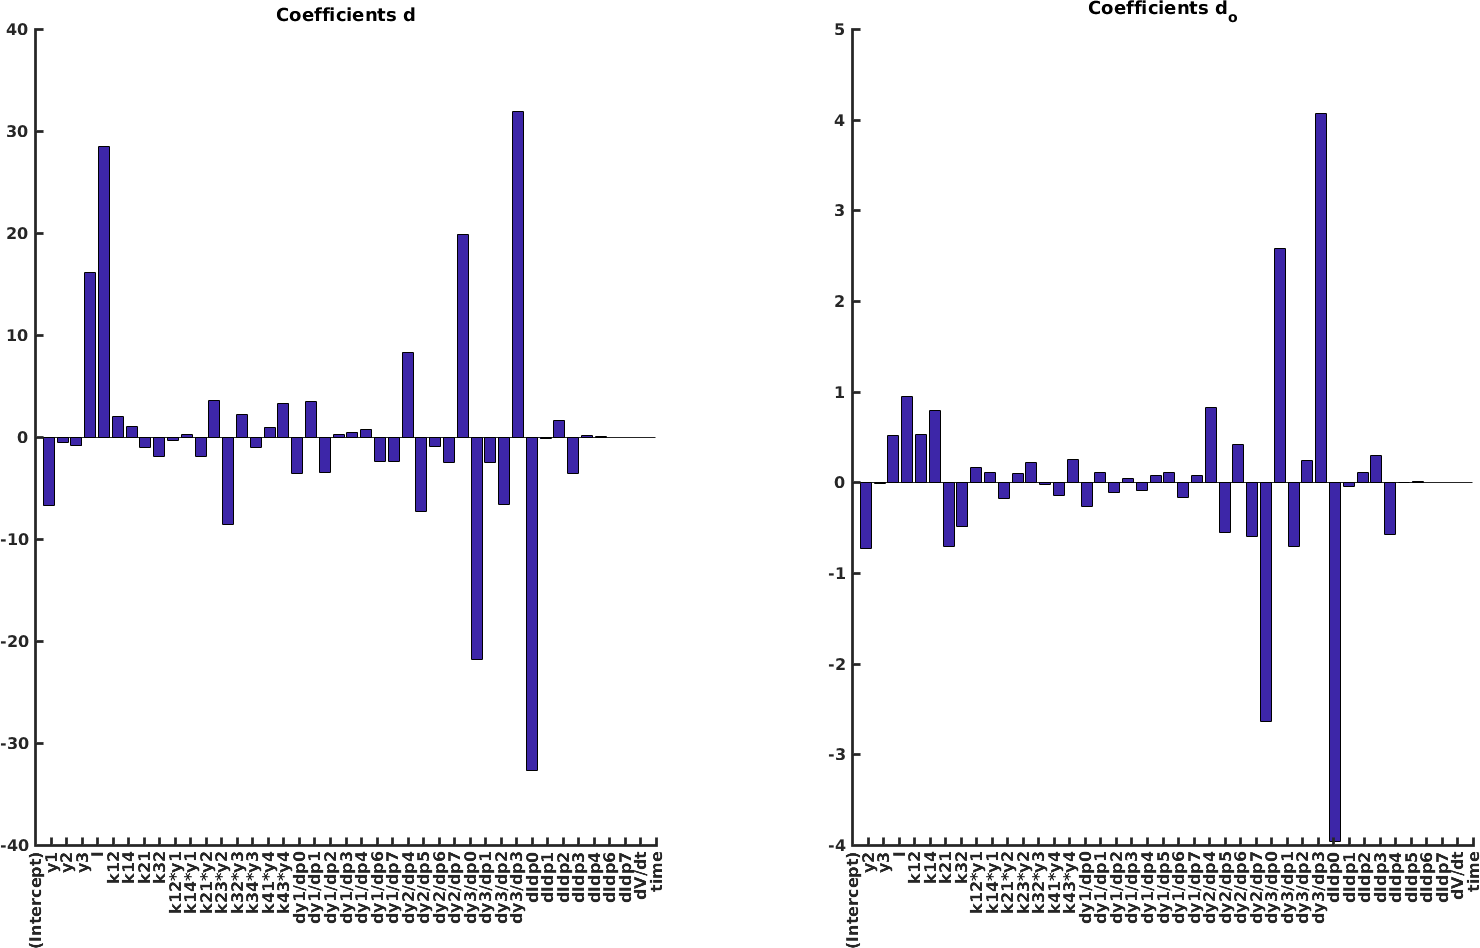
\includegraphics[scale=0.42]{Figures/StepwiseLM_OSW_AP_full_coefficients.png}
\caption{\textbf{Coefficients in the linear model of discrepancy constructed using StepwiseLM from the OSW protocol.} This plot shows the included parameters and coefficients for the model produced by StepwiseLM shown in Fig.~\ref{Fig_StepwiseLM_OSW_AP_full_discrepancy} and Fig.~\ref{Fig_StepwiseLM_OSW_AP_full_currents}. Coefficients for $d$ are shown on the left, and coefficients for $d_o$ are shown on the right.} 
\label{Fig_StepwiseLM_OSW_AP_full_coefficients}
\end{center}
\end{figure}

\clearpage

\begin{figure}[t]
\begin{center}
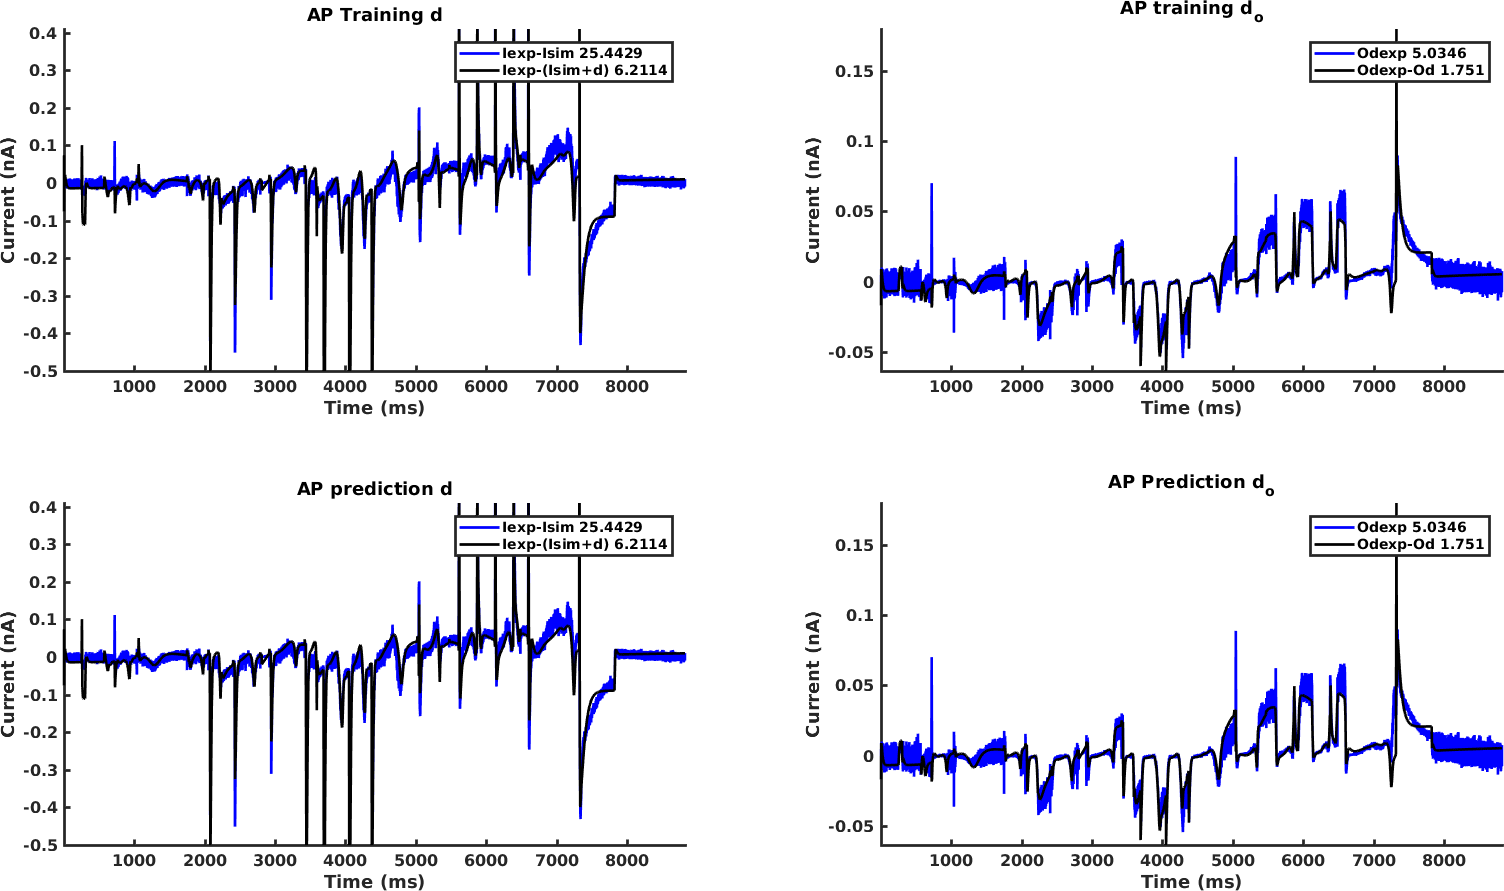
\includegraphics[scale=0.42]{Figures/StepwiseLM_AP_AP_full_discrepancy.png}
\caption{\textbf{Linear model of discrepancy constructed using StepwiseLM from the AP protocol.} These models of $d$ (left) and $d_o$ (right) were constructed using StepwiseLM on the entire AP trace (top), starting with all linearly independent predictors. The root mean square errors between the simulated and predicted traces are shown in the legends. Note that the top and bottom rows of this figure are the same. } 
\label{Fig_StepwiseLM_AP_AP_full_discrepancy}
\end{center}
\end{figure}

\begin{figure}[hb]
\begin{center}
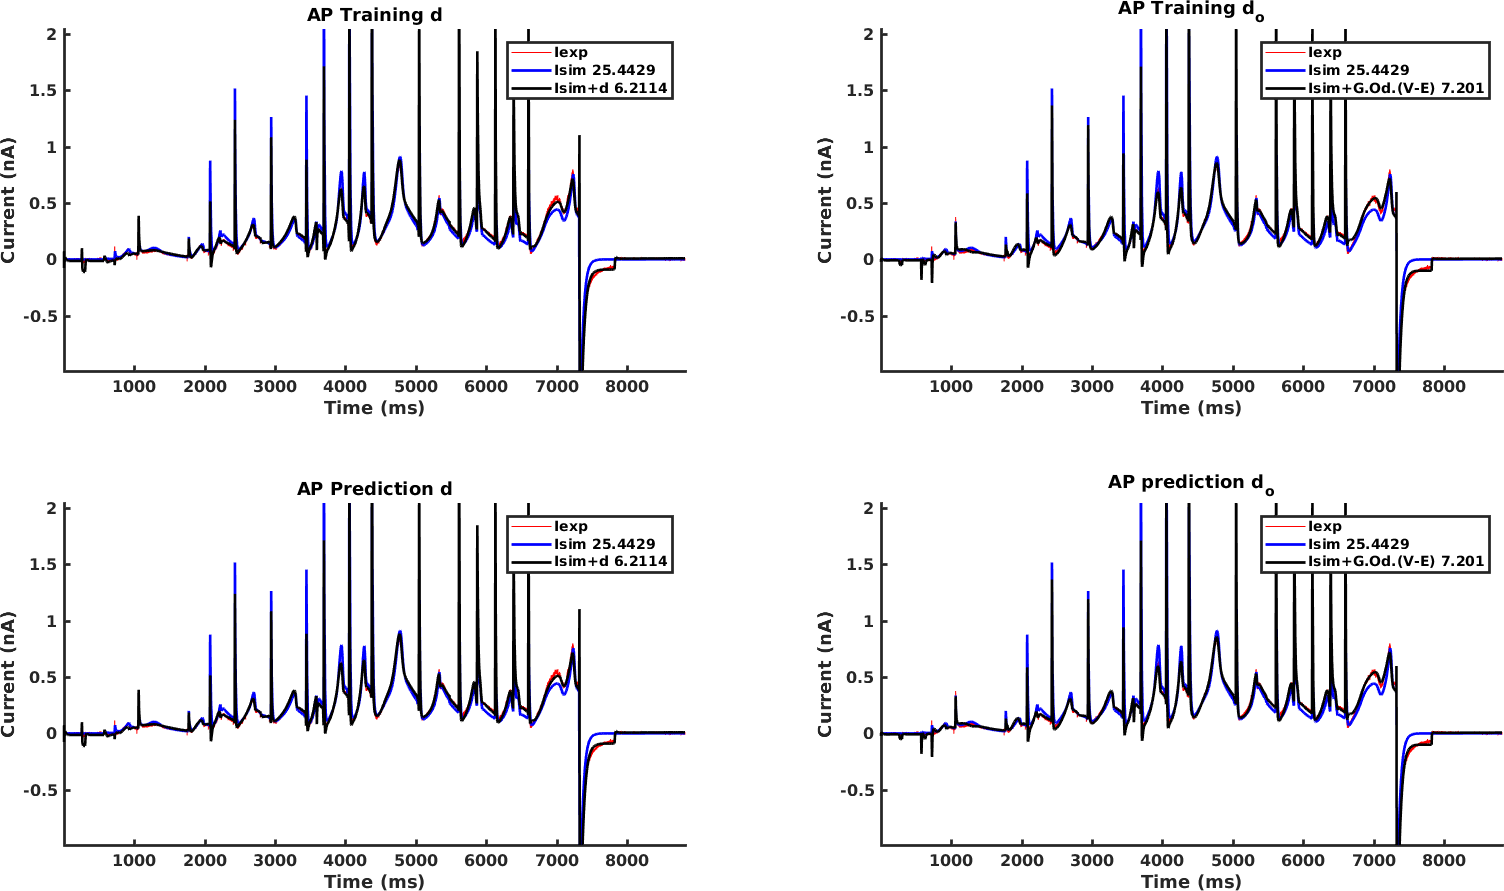
\includegraphics[scale=0.42]{Figures/StepwiseLM_AP_AP_full_currents.png}
\caption{\textbf{Corrected currents using a linear model of discrepancy constructed using StepwiseLM from the OSW protocol.} The models of $d$ (left) and $d_o$ (right) in Fig. ~\ref{Fig_StepwiseLM_AP_AP_full_discrepancy} have been incorporated into the simulation (blue line), giving a revised prediction for the AP protocol (black line). The sum of squared errors between the models and the data are shown in the legend.Note that the top and bottom rows of this figure are the same.}
\label{Fig_StepwiseLM_AP_AP_full_currents}
\end{center}
\end{figure}

\clearpage

\begin{figure}[t]
\begin{center}
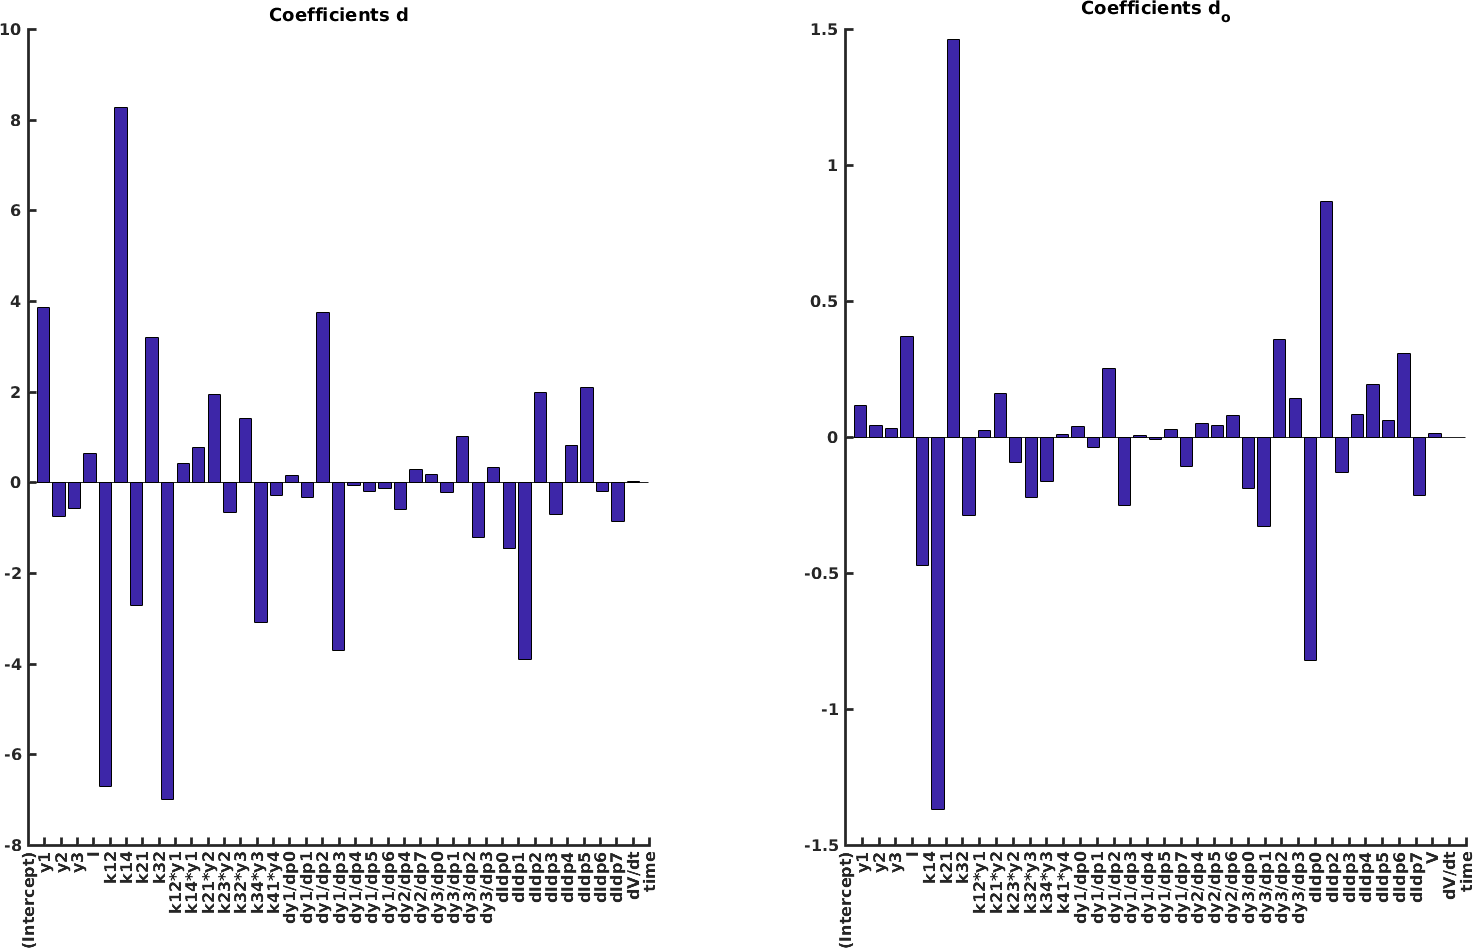
\includegraphics[scale=0.42]{Figures/StepwiseLM_AP_AP_full_coefficients.png}
\caption{\textbf{Coefficients in the linear model of discrepancy constructed using StepwiseLM from the AP protocol.} This plot shows the included parameters and coefficients for the model produced by StepwiseLM shown in Fig.~\ref{Fig_StepwiseLM_AP_AP_full_discrepancy} and Fig.~\ref{Fig_StepwiseLM_AP_AP_full_currents}. Coefficients for $d$ are shown on the left, and coefficients for $d_o$ are shown on the right.} 
\label{Fig_StepwiseLM_AP_AP_full_coefficients}
\end{center}
\end{figure}

\clearpage

\subsection{Artificial Data}
Given the disappointing results in Sections \ref{SubSec_Lasso_Discrepancy} and \ref{SubSec_StepwiseLM_Discrepancy} above, we performed a set of test studies to determine how well the methods could be expected to perform under these circumstances. The first test was to use the AP trace for training, thereby determining an `optimal' model - this approach places a bound on the quality of the fit that should be expected from the method applied - it is constructing a model using the prediction data as shown above. 

The second method we used to determine how effective the methods were likely to be was to generate artificial data. In this approach, we assume that our central hypothesis is true and that the discrepancy between the model and the data can be represented by a linear sum of the model-derived predictors in Section~\ref{SubSec_Predictors}. `Discrepancies' are generated by firstly choosing a random number of $n$ predictors between 1 and 20, and then randomly selecting $n$ predictors. These predictors are then summed with a constant linear coefficient so that the magnitude is comparable to the magnitude of the $d$ trace. Finally, Gaussian noise with mean 0 and standard deviation from the first 1000 time points in the $d$ trace is applied. The process was repeated in the absence of noise. Two examples constructed using LASSO are shown in Figs.~\ref{Fig_LassoArtificialExample}. We repeated this process 20 times and then recorded the relationship between the number of parameters in the model and the MSE between the true model's coefficients and the fitted model's coefficients. Non-included predictors were treated as having a coefficient value of zero. The results are shown in Fig.~\ref{Fig_BatchArtificialFits}, showing that the more parameters are included in the target model, the less likely the model is to be correct. Consequently, large models produced through this fitting method are unlikely to be reliable, consistent with the results shown when using the experimental data in the previous section.

\begin{figure}[t]
\begin{center}
\includegraphics[scale=0.42]{Figures/LassoArtificialExample1_TrainingVsPrediction.png} \hspace{1cm}
\includegraphics[scale=0.21]{Figures/LassoArtificialExample1_Coeffs.png} \newline \newline
\includegraphics[scale=0.42]{Figures/LassoArtificialExample2_TrainingVsPrediction.png} \hspace{1cm}
\includegraphics[scale=0.21]{Figures/LassoArtificialExample2_Coeffs.png}
\caption{\textbf{Example fits using LASSO to artificial data}. The fit of the model to the artificial data is shown on the left, and the coeffcicients in the constructed model and the original model are shown on the right.} 
\label{Fig_LassoArtificialExample}
\end{center}
\end{figure}

\begin{figure}[bt]
\begin{center}
\includegraphics[scale=0.42]{Figures/BatchFitToData.png}
\caption{\textbf{Effectiveness of LASSO and StepwiseLM at recovering artificial data}. The MSE between the original coefficients constructing the artificial model, and the coefficients of the fitted linear model is shown on the y axis, and the number of parameters included in the artificial model is shown on the x-axis. The left panel shows the results for LASSO and the right panel shows the results for StepwiseLM.} 
\label{Fig_BatchArtificialFits}
\end{center}
\end{figure}

\subsection{Conclusions}

The LASSO method tended to produce very small models, particularly for $d_o$. These models were not capable of predicting the discrepancy in the AP trace, even though the analysis in Fig.~\ref{Fig_BatchArtificialFits} suggests that they ought to be relatively reliable if they were detecting a real signal. The fact that these models are unreliable is consistent with them being inaccurate. It is notable that the difference between the folds in most cases is large relative to the MSE, which would suggest that the model is not particularly effective for prediction even within the training data, and explains why very small models tended to be chosen - the LASSO method could not conclude that the larger model with the smallest overall MSE was definitely better than a sparse model. This shows the value of K-fold cross-validation on the training data in any future application of similar methods. Conversely, StepwiseLM tended to produce large linear models which are likely to be untrustworthy based on the simulated data examples in Fig.~\ref{Fig_BatchArtificialFits}. Their lack of predictive function supports this view. We also note that the small discrepancy between the original parameterized model and the experimental data does not seem to be the source of the problem - in the cases where alternative protocols (EP, MWDD, OSW) were used to fit the linear model, the result tended to be worse than for the SW protocol.

It is striking that the two different methods, over multiple different datasets, are very rarely consistent in the predictors they include in the model, either between datasets or between methods. This finding further indicates that a true structural source for the discrepancy is not being successfully identified, as if a source of error were to exist amongst these variables it would be expected to be consistently included. It is also instructive to note that in the two cases where the model was constructed from the prediction data (AP protocol), the error could be reduced to a magnitude comparable to that in the SW protocol data prior to fitting. This is encouraging at first sight. However, the two constructed models are completely different and both very large. Furthermore, the error is much lower in StepwiseLM than LASSO, which may suggest a better model, or alternatively overfititng due to the lack of K-fold cross validation.

Based on the results shown above, we conclude that straightforward linear regression on predictors derived from the HH model equations is unlikely to be an effective method for predicting discrepancy. Unfortunately, this assertion is difficult to prove conclusively as we do not know the structure of the experimental data. Furthermore, in the trivial case where the discrepancy is included in the predictors then the method should always work. Taking these two facts together, we see that any proof without knowledge of how the data ought to behave is likely to be impossible. As mentioned in Section~\ref{Sec_FutureWork}, an approach based on simulations of different model structures may yield insights, but the results presented above suggest that the effort may be better spent elsewhere if practical application of the method within the CiPA framework is desired. 

\section{Parameter Fits Using Alternate Protocols}\label{Sec_AltProtocols}

\subsection{Introduction}
All of the above results consider model discrepancy between a model parameterized to one data set - the SW protocol. In this section, we attempted to determine whether the choice of fitting protocol could provide information about model discrepancy through changing parameters in different regions of parameter space.

\subsection{Methods}
We followed the parameter estimation methods used by Beattie et al for the SW protocol. Briefly, this consisted of a global search using the CMA-ES algorithm from different start points to detect local minima in the parameter space, as measured by the MSE between simulation and experimentally recorded current. Starting from the parameter set with least MSE as determined by the CMA-ES procedure, Markov Chain Monte Carlo (MCMC) Sampling was used to ensure a local optimum has been reached. In all cases, the HH model as used by Beattie et al (Eqns.~\eqref{Eq_dCdt}-\eqref{Eq_I_hh}) was used in the fitting procedure \cite{Beattie2018}.

Fits were performed using the following pacing protocols: AP, OSW, EP, MWDD. Additionally, the original method of Beattie et al was modified to allow the fitting of multiple protocols simultaneously, and was applied to the following combinations of protocols. The log-likelihood function used for optimization is as follows:
\begin{align}
\sum_{i=1}^P \Big\{ -0.5  N_i \log( 2 \pi \sigma_i^2 )-0.5 \frac{1}{\sigma_i^2}\sum_{j=1}^{N_i}(I_{exp,i,j}-I_{sim,i,j})^2 \Big\},
\end{align}
where $P$ is the number of protocols, $N_i$ is the number of data points recorded for protocol $i$, $\sigma_i$ is the standard deviation of the first 200 ms of current recorded for protocol $i$, $I_{exp,i,j}$ is the $j$\textsuperscript{th} time point recorded experimentally for protocol $i$, and $I_{sim,i,j}$ is the $j$\textsuperscript{th} time point of the simulation of protocol $i$ using the current parameter set. Capacitative spikes were disregarded as shown in Fig.~\ref{Fig_Protocols}.

When determining whether a parameter set produced realistic transition rates, we determined the maximum transition rates for each protocol $i$ as follows:
\begin{align}
r_i = \max_{V_i} \big( \ k_1(V_i), k_2(V_i), k_3(V_i), k_4(V_i) \ \big) 
\end{align}
where $V_i$ is the voltage in protocol $i$ and the rates $k_m$ are as defined above. The transition rates are then deemed realistic if 
\begin{align}
\max_i \big( r_i \big) \in \left[ 1.67e{-5} \ 1000  \right].
\end{align}
Parameter upper and lower bounds were protocol independent and determined in the same manner as by Beattie et al. 

When illustrating goodness of fit to a protocol in the Results section, the Root Mean-Squared Error (RMSE) for protocol $i$ is used,
\begin{align}
\text{RMSE}_i & = \sqrt{ \frac{1}{N_i}\sum_{i=1}^{N_i}(I_{exp,i,j}-I_{sim,i,j})^2 }.
\end{align}

\subsection{Results}

The RMSEs for each fit and for each of the five fitting protocols used are shown in Table~\ref{Tab_MSE_Fitted}. From this table, it can be seen that fits to either AP and SW reduce in substantially better fits to the target protocol than any of EP, MWDD, or OSW (diagonal of first five rows). The worst fit to a target protocol was obtained when fitting to OSW. Of the single protocols, the SW protocol gives the best prediction for the AP protocol (third column, rows 1,3,4,5). The OSW protocol gives the worst prediction of the AP protocol. For each of the 5 protocols, the fit to the fitting protocol and its prediction of the AP protocol is shown in Fig.~\ref{Fig_SWfit}-\ref{Fig_OSWfit}. When fitting to the AP protocol, its prediction of the SW protocol is shown in Fig.~\ref{Fig_APfit}. Combining the AP and SW protocols lead to a compromise fit, that, while less good than the original SW fit or the AP fit alone, produced a dramatic improvement in the quality of fit to both, as shown in Fig.~\ref{Fig_AP_SWfit}. However, the fit to EP, MWDD or OSW is not substantially better than for the fits to the AP and SW protocols individually. Combining AP and EP also lead to improvements over the EP protocol alone, although these were more modest than for the AP and SW combination. Combining SW and OSW did not lead to satisfactory fits.

\begin{table}
\caption{RMSE of fitted HH models for different protocols}
\centering
\begin{tabular}{|c|c|c|c|c|c|}
\hline 
 Fitting Protocol & SW & AP & EP & MWDD & OSW \\ [0.5ex]
\hline 
\hline
SW \cite{Beattie2018} & 0.032 & 0.087 & 0.140 & 0.327 & 0.557 
 \\
\hline 
AP & 0.132 & 0.035 & 0.179 & 0.360 & 0.415  \\ 
\hline 
EP & 0.101 & 0.146 & 0.100 & 0.216 & 0.654  \\ 
\hline 
MWDD & 0.138 & 0.144 & 0.154 & 0.135 & 0.330 
\\ 
\hline 
OSW & 0.218 & 0.368 & 0.148 & 0.390 & 0.144 
 \\ 
\hline 
AP \& SW & 0.042 & 0.048 & 0.143 & 0.334 & 0.374 
 \\
\hline 
AP \& EP & 0.084 & 0.077 & 0.112 & 0.253 & 0.394 
 \\
\hline
SW \& OSW & 0.150 & 0.180 & 0.156 & 0.360 & 0.166 
 \\
\hline
\end{tabular} 
\label{Tab_MSE_Fitted}
\end{table}

\begin{figure}[ht]
\begin{center}
\includegraphics[scale=0.42]{Figures/Fig_hh_16713110_FP_sine_wave_CP_sine_wave.png}
\includegraphics[scale=0.42]{Figures/Fig_hh_16713110_FP_sine_wave_CP_ap.png}
\caption{\textbf{Fit to SW protocol}. The fit of the HH model (blue) to experimental data (red) from the SW protocol  for Cell 5 is shown on the left hand side. Using the same parameter set, the prediction of the current from the AP protocol (blue) and the corresponding experimentally recorded current are shown on the right hand side.} 
\label{Fig_SWfit}
\end{center}
\end{figure}

\begin{figure}[hb]
\begin{center}
\includegraphics[scale=0.42]{Figures/Fig_hh_16713110_FP_equal_proportions_CP_equal_proportions.png}
\includegraphics[scale=0.42]{Figures/Fig_hh_16713110_FP_equal_proportions_CP_ap.png}
\caption{\textbf{Fit to EP protocol}. The fit of the HH model (blue) to experimental data (red) from the EP protocol  for Cell 5 is shown on the left hand side. Using the same parameter set, the prediction of the current from the AP protocol (blue) and the corresponding experimentally recorded current are shown on the right hand side.} 
\label{Fig_EPfit}
\end{center}
\end{figure}

\begin{figure}[ht]
\begin{center}
\includegraphics[scale=0.42]{Figures/Fig_hh_16713110_FP_maz_wang_div_diff_CP_maz_wang_div_diff.png}
\includegraphics[scale=0.42]{Figures/Fig_hh_16713110_FP_maz_wang_div_diff_CP_ap.png}
\caption{\textbf{Fit to MWDD protocol}. The fit of the HH model (blue) to experimental data (red) from the MWDD protocol  for Cell 5 is shown on the left hand side. Using the same parameter set, the prediction of the current from the AP protocol (blue) and the corresponding experimentally recorded current are shown on the right hand side.} 
\label{Fig_MWDDfit}
\end{center}
\end{figure}

\begin{figure}[hb]
\begin{center}
\includegraphics[scale=0.42]{Figures/Fig_hh_16713110_FP_original_sine_CP_original_sine.png} 
\includegraphics[scale=0.42]{Figures/Fig_hh_16713110_FP_original_sine_CP_ap.png}
\caption{\textbf{Fit to OSW protocol}. The fit of the HH model (blue) to experimental data (red) from the OSW protocol  for Cell 5 is shown on the left hand side. Using the same parameter set, the prediction of the current from the AP protocol (blue) and the corresponding experimentally recorded current are shown on the right hand side.} 
\label{Fig_OSWfit}
\end{center}
\end{figure}

\begin{figure}[ht]
\begin{center}
\includegraphics[scale=0.42]{Figures/Fig_hh_16713110_FP_ap_CP_ap.png}
\includegraphics[scale=0.42]{Figures/Fig_hh_16713110_FP_ap_CP_sine_wave.png}
\caption{\textbf{Fit to AP protocol}. The fit of the HH model (blue) to experimental data (red) from the AP protocol  for Cell 5 is shown on the left hand side. Using the same parameter set, the prediction of the current from the SW protocol (blue) and the corresponding experimentally recorded current are shown on the right hand side.} 
\label{Fig_APfit}
\end{center}
\end{figure}

\begin{figure}[hb]
\begin{center}
\includegraphics[scale=0.42]{Figures/Fig_hh_16713110_FP_ap_sine_wave_CP_sine_wave.png}
\includegraphics[scale=0.42]{Figures/Fig_hh_16713110_FP_ap_sine_wave_CP_ap.png}
\caption{\textbf{Fit to AP and SW protocols}. The fit of the HH model (blue) to experimental data (red) from the SW and AP protocols for Cell 5 is shown on the left hand side, compared to the data for the SW protocol. Using the same parameter set, the simulation of the current from the AP protocol (blue) and the corresponding experimentally recorded current are shown on the right hand side.} 
\label{Fig_AP_SWfit}
\end{center}
\end{figure}

\begin{figure}[hb]
\begin{center}
\includegraphics[scale=0.42]{Figures/Fig_hh_16713110_FP_ap_sine_wave_CP_ap_zoom.png}
\caption{\textbf{Fit to AP and SW protocols: focus on current following AP upstroke}. The fit of the HH model from the SW and AP protocols (blue, solid line) and from the SW protocol alone (blue, dashed line), for Cell 5 is shown on the left hand side, compared to the current data for the AP protocol (red line). Currents following three AP upstrokes are shown.} 
\label{Fig_AP_SWzoomfit}
\end{center}
\end{figure}

One notable result of the fit to the SW and AP combined is that it demonstrates the existence of a potentially better fit for both protocols than that produced by SW alone, although the fit to the SW alone is slightly worse. In particular, this fit improves the fitting of the decay of the current after the AP upstroke in the AP protocol, which contributes to large discrepancies in the AP protocol (zoom in Fig.~\ref{Fig_AP_SWzoomfit}). However, the error in the early after-depolarization part of the AP trace remains large (Fig.~\ref{Fig_AP_SWfit}, bottom, around 7000ms).

Parameter sets from each set of fitting protocols are shown in Table.~\ref{Tab_Fitted_Parameters}. Conductance ($G$) varied wildly between the parameter fits, with AP, MWDD, and OSW coming close to the maximum allowed conductance. In the case of the AP protocol, this may be explained by the lack of an activation step prior to the action potential component of the protocol, however this step is present in both the OSW and MWDD protocols. Combining AP or OSW with SW reduced the estimate for the protocol. In contrast, EP lead to a lower estimate of the conductance than found in the SW. The kinetic rate parameters do not appear to follow a pattern. However, the kinetic parameters for SW, AP and AP \& SW are all of the same order of magnitude as one another, which is not true for the other protocols (EP, MWDD, OSW).

\begin{table}
\caption{Fitted HH model parameters}
\centering
\resizebox{\textwidth}{!}{%
\begin{tabular}{|c|c|c|c|c|c|c|c|c|c|}
\hline 
Fitting Protocol & $G$ & $P_0$ & $P_1$ & $P_2$ & $P_3$ & $P_4$ & $P_5$ & $P_6$ & $P_7$ \\ [0.5ex]
\hline 
\hline
SW \cite{Beattie2018} & 0.152395 & 0.000226 & 0.069925 & 0.000034 & 0.054616 & 0.087328 & 0.008914 & 0.005152 & 0.031583  \\ 
\hline 
AP & 0.599747 & 0.000063 & 0.047988 & 0.000023 & 0.055198 & 0.101544 & 0.016342 & 0.006023 & 0.022413 
 \\ 
\hline 
EP & 0.126691 & 0.002110 & 0.040174 & 0.000131 & 0.039128 & 0.084381 & 0.003305 & 0.003411 & 0.032497  \\ 
\hline 
MWDD & 0.611997 & 0.003991 & 0.025138 & 0.000593 & 0.026240 & 0.196518 & 0.000000 & 0.001292 & 0.028238  \\ 
\hline 
OSW & 0.612000 & 0.000078 & 0.018201 & 0.000000 & 0.097087 & 0.170079 & 0.026229 & 0.001162 & 0.048377  \\ 
\hline 
AP \& SW & 0.159141 & 0.000195 & 0.068248 & 0.000011 & 0.063159 & 0.119212 & 0.012568 & 0.006842 & 0.026522 \\
\hline 
AP \& EP & 0.112754 & 0.001071 & 0.045607 & 0.000126 & 0.039605 & 0.109146 & 0.013584 & 0.006111 & 0.027252  \\
\hline 
SW \& OSW & 0.106054 & 0.000298 & 0.050493 & 0.000001 & 0.083926 & 0.166419 & 0.026477 & 0.002109 & 0.044508 
 \\
\hline 
\end{tabular} 
}
\label{Tab_Fitted_Parameters}
\end{table}

\subsection{Conclusions}

Based on the above results for fitting, we conclude that, of the protocols studied, the SW protocol produces the best fits in terms of predicting the AP protocol. Fitting to the AP protocol directly of course gives a better result for the AP, but the results for predicting the SW protocol were worse in this case. However, fitting to both the AP and SW protocol produced fits of quality nearing that for the direct fits to either the SW or the  AP protocols with one parameter set. This result suggests that, while the parameters fitted for the SW protocol alone have been shown to be 'optimal' for that protocol by Beattie et al \cite{Beattie2018}. In particular, this finding suggests that the difference between simulations and experiment following the AP upstrokes may not be down to measurement error resulting from a pacing artefact, but may be (partially) accounted for by improved parameterisation. However, errors elsewhere in the trace, and the discrepancy in the AP alone fit, continue to support the hypothesis that prediction errors cannot entirely be fixed by parameterisation and that some degree of model error is still present. These results confirm that, while further improvement of the SW protocol may be possible, particularly in terms of capturing post-upstroke behaviour, it is the best choice of teh protocols tested thus far for predicting currents induced by AP-like waveforms.

It is worthwhile to speculate as to why the SW protocol outperforms other protocols at predicting the AP protocol currents. Phase-plane analysis (Dr.~Clerx) suggests that the AP and SW protocols exist in a similar region of phase space, at least when fitted to the SW protocol data. This finding may suggests that the SW and AP protocols are perhaps more similar than they first appear, in terms of the model behaviours elicited. No fitting protocol was able to reproduce quantitatively the behaviour produced during the early after-depolarization at the end of the AP trace, including the AP protocol itself. This suggests that the channel kinetics are inadequately represented in this kind of behaviour, indicative of model discrepancy in an area crucial for arrhythmogenesis.

\clearpage

\section{Discrepancy Between Alternate Model Structures}\label{Sec_ModelDiscrepancy}

\subsection{Introduction}
Understanding model discrepancy directly from experimentally recorded currents is extremely challenging, as the gating kinetics of the hERG channel remain a source of scientific debate. This can be demonstrated by studying the range of different kinetic model structures shown in Beattie et al. \cite{Beattie2018}. As existing methods for evaluating the influence of model discrepancy on simulation results rely on having some prior idea of factors omitted from the model \cite{Strong2014}, we therefore decided to investigate how model discrepancy between different models trained on the same data would manifest itself. We therefore performed two experiments - one to fit an $mh$ model to the current generated by the Wang model, which has a completely different structure, and one whereby we fit four different models all based on the Hodgkin-Huxley equations to the SW protocol. Each of these models can be thought of as adding additional closed and/or inactive states to the HH model. 

\subsection{Methods}
In this section, we used two different sets of target currents for fitting, based on the SW protocol. The first, used to fit an $mh$ model (Eqns.~\eqref{Eq_dmdt}-\eqref{Eq_mh}), was the current generated by the Wang model when fitted to the SW protocol (Wang$_\text{SW}$), as can be found in the supplement of the paper by Beattie et al \cite{Beattie2018}. The second set of data was the original SW protocol data recorded from cell 5, to which each of the $mh$, $m^2h$, $m^3h$, $m^4h$, and $m^2h^2$ models (Eqns.~\eqref{Eq_mh}-\eqref{Eq_m2h2}) was fitted. The fitting method was the same as shown in Section \ref{Sec_AltProtocols}. Note that the output of the $mh$ model is identical to the HH model in terms of current generated when the same parameter sets are used.

\subsection{Results}

The fit of the $mh$ model to the Wang model is shown in  Fig.~\ref{Fig_SW_Wang}, with a zoom in Fig.~\ref{Fig_SW_Wang_Zoom}. The models produce extremely similar outputs, however some evidence of model discrepancy can be found during the activation and deactivation steps, where the Wang$_\text{SW}$ model is able to reproduce behaviours that the HH model cannot. Fitted parameters for the $mh$ model to the Wang$_\text{SW}$ model are shown in Table~\ref{Tab_Fitted_Parameters_Wang}. It is notable that the parameters of the $mh$ model when fitted to the Wang$_\text{SW}$ model instead of the experimentally recorded current from the SW protocol data have barely changed, indicating that the model is barely changing its fit from the original fit to the SW protocol. This indicates that, from the fitting algorithm point of view, the SW protocol data and Wang$_\text{SW}$ are almost indistinguishable, as confirmed by their similar behaviour for the AP protocol shown in Fig.~\ref{Fig_AP_Wang}. The Wang$_\text{SW}$ model and the HH model, however, begin to diverge from one another when simulating the AP protocol. This finding indicates that model discrepancy may be detectable when using predictions based on data not used for fitting. However, as concluded above, linear regression methods are unlikely to detect this difference. 

\begin{figure}[ht]
\begin{center}
\includegraphics[scale=0.42]{Figures/Fig_mh_16713110_FP_sine_wave_wang_CP_sine_wave_wang.png}
\caption{\textbf{Fit to Wang$_\text{SW}$}. The simulation of the Wang model fitted to the SW protocol (Wang$_\text{SW}$) is shown in red. The fit of the $mh$ model to Wang$_\text{SW}$ is shown in blue. For comparison, the original Beattie et al model is shown in blue dashes.} 
\label{Fig_SW_Wang}
\end{center}
\end{figure}

\begin{figure}[hb]
\begin{center}
\includegraphics[scale=0.42]{Figures/Fig_mh_16713110_FP_sine_wave_wang_CP_sine_wave_wang_zoom.png}
\caption{\textbf{Fit to Wang$_\text{SW}$, with zoom}. The simulation of the Wang model fitted to the SW protocol (Wang$_\text{SW}$) is shown in red. The fit of the $mh$ model to Wang$_\text{SW}$ is shown in blue. For comparison, the original Beattie et al model is shown in blue dashes. } 
\label{Fig_SW_Wang_Zoom}
\end{center}
\end{figure}

\begin{table}
\caption{Fitted HH model parameters to the Wang model}
\centering
\resizebox{\textwidth}{!}{%
\begin{tabular}{|c|c|c|c|c|c|c|c|c|c|}
\hline 
Fitting Protocol & $G$ & $P_0$ & $P_1$ & $P_2$ & $P_3$ & $P_4$ & $P_5$ & $P_6$ & $P_7$ \\ [0.5ex]
\hline 
\hline
SW \cite{Beattie2018} & 0.152395 & 0.000226 & 0.069925 & 0.000034 & 0.054616 & 0.087328 & 0.008914 & 0.005152 & 0.031583  \\ 
\hline 
HH$_\text{SW}$ & 0.149807 & 0.000223 & 0.068167 & 0.000030 & 0.055608 & 0.101196 & 0.010718 & 0.006310 & 0.030265 \\ 
\hline 
\end{tabular} 
}
\label{Tab_Fitted_Parameters_Wang}
\end{table}

\begin{figure}[hb]
\begin{center}
\includegraphics[scale=0.42]{Figures/Fig_mh_16713110_FP_sine_wave_wang_CP_ap_wang.png}
\caption{\textbf{Fit to Wang$_\text{SW}$ used to simulate the AP protocol}. The Wang$_\text{SW}$ model simulated for the AP protocol is shown in red. The fit of the $mh$ model to Wang$_\text{SW}$ is shown in blue and used to simulate the AP protocol. For comparison, the original Beattie et al model is shown in blue dashes.} 
\label{Fig_AP_Wang}
\end{center}
\end{figure}

Parameter fits for the SW protocol using the $mh$ ,$m^2h$, $m^3h$, $m^4h$ and $m^2h^2$ models are shown in Table \ref{Tab_Fitted_Parameters_mh}. Traces of the change in model structure can be seen in the changes in the parameters. Parameters influencing the closed to open transition represented by $m$ in the $mh$ formulation ($P_0$ - $P_3$) show considerable differences between the $mh$, $m^2$, $m^3h$ and $m^4h$ models, while the parameters representing the active - inactive transition represented by $h$ remain relatively constant ($P_4$ - $P_7$). By contrast, there are large changes from the $mh$ model in both sets of parameters for the $m^2h^2$ model.Furthermore, voltage dependence parameters tend to decrease in magnitude as the exponent of their related variable increases. Conductance increases with the powers in the model, consistent with the effect of an exponent applied to a value between 0 and 1 reducing the open probability. 

Plots of the resulting model simulations for the SW protocol are shown in Fig.~\ref{Fig_mh_SW}, with a zoom in Fig.~\ref{Fig_mh_SW_Zoom}. The fits for each model are similar, however distinct behaviour appear during the activation step where the unrealistic early spike in current in the $mh$ step is reduced in the models with exponents. However, this comes at a price of a slower accumulation of current during this step. Otherwise, the fits are very similar. In the prediction simulations using the AP protocol (Fig.~\ref{Fig_mh_AP} and Fig.~\ref{Fig_mh_AP_Zoom}), it can again be appreciated that all five models behave in a qualitatively similar way, although discrepancy does begin to emerge. In general, the models with larger exponents tend to over-estimate the current (perhaps due to the increased conductance), while models with lower exponents tend to under-estimate the current. RMSE values for the fits are shown in Table \ref{Tab_RMSE_mh}. In terms of RMSE, while the $mh$ model does provide the best fit to the SW data, the prediction of the AP data is similar for the $mh$, $m^2h$, $m^3h$ and $m^4h$ models. The $m^2h^2$ model provides a worse prediction overall.

\begin{table}
\caption{Fitted $mh$ model parameters}
\centering
\resizebox{\textwidth}{!}{%
\begin{tabular}{|c|c|c|c|c|c|c|c|c|c|}
\hline 
Fitting Protocol & $G$ & $P_0$ & $P_1$ & $P_2$ & $P_3$ & $P_4$ & $P_5$ & $P_6$ & $P_7$ \\ [0.5ex]
\hline 
\hline
$mh$ & 0.152397 & 0.000226 & 0.069922 & 0.000034 & 0.054615 & 0.087329 & 0.008915 & 0.005152 & 0.031582 
  \\ 
\hline 
$m^2h$ & 0.157950 & 0.001316 & 0.029060 & 0.000044 & 0.047010 & 0.085411 & 0.009117 & 0.004852 & 0.030882 
 \\ 
\hline 
$m^3h$ & 0.167375 & 0.001881 & 0.018868 & 0.000053 & 0.042376 & 0.086311 & 0.009076 & 0.004655 & 0.030357 
 \\ 
\hline 
$m^4h$ & 0.172830 & 0.002181 & 0.015171 & 0.000054 & 0.039888 & 0.086073 & 0.009009 & 0.004493 & 0.030211 
 \\ 
\hline 
$m^2h^2$ & 0.191411 & 0.000986 & 0.042141 & 0.000028 & 0.050956 & 0.055119 & 0.001509 & 0.014950 & 0.023350 
 \\ 
\hline 
\end{tabular} 
}
\label{Tab_Fitted_Parameters_mh}
\end{table}

\begin{figure}[ht]
\begin{center}
\includegraphics[scale=0.42]{Figures/Fig_mh_family_16713110_FP_sine_Wave_CP_sine_wave.png}
\caption{\textbf{Fits to the SW protocol using alternative $mh$ model structures}. Simulations of the $mh$ ,$m^2h$, $m^3h$, $m^4h$ and $m^2h^2$ models fitted to the SW protocol for cell 5 are shown. Experimental data is shown in red.} 
\label{Fig_mh_SW}
\end{center}
\end{figure}

\begin{figure}[hb]
\begin{center}
\includegraphics[scale=0.42]{Figures/Fig_mh_family_16713110_FP_sine_wave_CP_sine_wave_zoom.png}
\caption{\textbf{Fits to the SW protocol using alternative $mh$ model structures - zoomed in}.  Simulations of the $mh$ ,$m^2h$, $m^3h$, $m^4h$ and $m^2h^2$ models fitted to the SW protocol for cell 5 are shown. Experimental data is shown in red.} 
\label{Fig_mh_SW_Zoom}
\end{center}
\end{figure}

\begin{figure}[ht]
\begin{center}
\includegraphics[scale=0.42]{Figures/Fig_mh_family_16713110_FP_sine_Wave_CP_ap.png}
\caption{\textbf{Prediction of the AP protocol using alternative $mh$ model structures}. Simulations of the $mh$ ,$m^2h$, $m^3h$, $m^4h$ and $m^2h^2$ models fitted to the SW protocol for cell 5 are shown. Experimental data is shown in red.} 
\label{Fig_mh_AP}
\end{center}
\end{figure}

\begin{figure}[hb]
\begin{center}
\includegraphics[scale=0.42]{Figures/Fig_mh_family_16713110_FP_sine_wave_CP_ap_zoom.png}
\caption{\textbf{Prediction of the AP protocol using alternative $mh$ model structures - zoomed in}.  Simulations of the $mh$ ,$m^2h$, $m^3h$, $m^4h$ and $m^2h^2$ models fitted to the SW protocol for cell 5 are shown. Experimental data is shown in red.} 
\label{Fig_mh_AP_Zoom}
\end{center}
\end{figure}

\begin{table}
\caption{RMSE for $mh$ models}
\centering
\resizebox{\textwidth}{!}{%
\begin{tabular}{|c|c|c|c|c|c|
}
\hline 
Protocol & $mh$ & $m^2h$ & $m^3h$ & $m^4h$ & $m^2h^2$ \\ [0.5ex]
\hline 
\hline
SW & 0.031694 & 0.039017 & 0.044552 & 0.047805 & 0.044960  \\ 
\hline 
AP & 0.086661 & 0.087106 & 0.086366 & 0.086869 & 0.102761  \\ 
\hline 
\end{tabular} 
}
\label{Tab_RMSE_mh}
\end{table}

\subsection{Conclusions}

Model discrepancy can be visualised in parameters when a comparison between model structures is possible. The family of $mh$ models are all comparable in structure and show a clear pattern in the variation in their parameters as a result of fitting, whilst producing almost indistinguishable simulations of the fitted data. However, when model parameters are not directly comparable, the failure of linear regression as a method for detecting model discrepancy presents challenges. In the data from fitting the HH model to the Wang$_\text{SW}$ model, we can observe the discrepancy in the AP simulations despite the extreme similarity of the two fits for the SW protocol. However, we still lack a method for determining the cause of this discrepancy at present when the structures are eitehr different or unknown. A further issue with the fitting to the Wang$_\text{SW}$ data can be seen in that the parameters of the fitted HH model barely differ from the model generated by Beattie et al. This finding suggests that we may not have fitted to the Wang$_\text{SW}$ as such, as the HH model cannot distinguish between this data set and the original experimental data. We may therefore ask how meaningful the fit to the model data directly is, as opposed to simply considering two optimally fitted models to the same data as being `the same'.

\clearpage

\section{Future Work}\label{Sec_FutureWork}

\subsection{Detecting Discrepancy}

In this report, we have described how linear regression as a method fails to allow us to predict discrepancy between a model and experimental data, and have shown that two popular methods may not be able to detect discrepancies of this kind. Consequently, we must look for alternative methods for detecting model discrepancy in the future. One proposal is to use methods that allow us to track the time dependency of the model, allowing us to monitor how they will change over time. In particular, the results for the SW+AP fit suggest that different parameter sets may give better or worse fits at different points in the experimental data trace. Consequently, we may need to have a representation of discrepancy that can be updated dynamically. 

One method that may be able to address the dynamic nature of the discrepancy while updating the state of the model is the Kalman Filter \cite{Reich2015}. Using a Kalman filter, model variables can be updated and changed through time in response to differences with a target trace. By treating parameters as variables with derivative 0, they can be included into the Kalman filter paradigm. The Kalman filter is an attractive alternative to whole-trace fitting as it allows for changes in a variable or parameter value to continue to have an effect from that point onwards. Using the idea that different components of the data may be fitted by different sets of parameters, we envisage running the filter over the same data set multiple times until a `steady state' is reached, where the Kalman filter performs the same operations on each run in terms of changing states and parameters. Points where parameters shift from one regime to another are likely to then represent regions where the chosen model structure cannot represent both behaviours using one parameter set, i.e. indicate model structural discrepancy. Using the Kalman filter to predict the discrepancy in a prediction trace such as the AP protocol data in Beattie et al \cite{Beattie2018} is likely to be more challenging as it is not clear how the filter would be `trained' \textit{a priori}.

The results for the $mh$ models in Section \ref{Sec_ModelDiscrepancy} demonstrate that model parameter changes are likely to follow some logic when model structures are comparable. Consequently, we would propose that future research into model discrepancy should start from this point - models with comparable structures such as the family of $mh$ models used here. In this case, some relation should be expected between the parameters fitted to the different models, and an important first step for any method for detecting structural discrepancy would be to be able to predict these changes. An additional observation is that the conductance may confound some of these predictions and so it may be more beneficial to fix the value for all fits in the first instance to allow a tighter focus on model structure. In a similar vein, future work should consider redoing Section \ref{Sec_AltProtocols} using a fixed conductance value, as this may enable closer comparison between kinetic parameters and consequently more insight into model structural discrepancy. A further advantage of using models with known structural discrepancies is that this will allow us to assess how far understanding model discrepancy in the training data (SW) allows us to predict the resulting discrepancy in the prediction (AP) data.

One disadvantage of the $m^kh$ models studied in Section \ref{Sec_ModelDiscrepancy} is that they add additional closed states whose parameters are directly related to one another. It may therefore be advantageous to break this relationship. One possibility would be to consider models of the form C-O-I, C-C-O-I, and so on, where the transition from inactive to closed is not present, yet the form of the model remains simple. Models of increasing size could be considered in a similar manner to Section \ref{Sec_ModelDiscrepancy}, with the additional possibility of investigating the influence of over-fitting and parameter degeneracy as models become large. 

\subsection{Representations of discrepancy}

In this study, we have considered two different definitions of discrepancy between simulated and experimental currents, one additive and one incorporated into the open probability (see Eqs.~\eqref{discrepancy_d} and \eqref{discrepancy_do}). In general, the regression methods described in Section \ref{Sec_ModelDiscrepancy} performed less well using the discrepancy in open probability rather than the simple additive definition of discrepancy. However, for understanding the influence of structural discrepancy in different settings, it may be necessary to consider expanding the definition of structural discrepancy, for example by adding a discrepancy term to each model state. Care should be taken so that each state remains positive and the sum of states sum to one - essentially this means that the sum of the discrepancies mustbe zero. Alternatively, discrepancy could be represented by adding a single `discrepant' state to the parameterised model, and using either direct fitting or Kalman filtering to determine its state occupancy throughout the trace. A major challenge for these methods will be that the only directly observable state of the model is the open probability, through the current. This represents another argument in favour of performing synthetic experiments as a first step before attempting to use this form of structural discrepancy to redesign existing models based on experimental data.

The majority of the above discussion addresses the understanding of structural uncertainty, on the assumption that a better fit to data will allow us to make a more accurate prediction of currents in experimental data. However, the quality of the fit to the SW protocol (away from the activation and deactivation steps) is so high as to suggest that this may not be possible. In this context, it may be worth considering a second protocol for training the discrepancy model, which is then used with the original model to simulate the prediction model. In this context, the results in Section~\ref{Sec_AltProtocols} seem relevant because the HH model produced poorer fits to the OSW, EP or MWDD protocols than it did to either the SW or the AP protocols, indicating that these protocols contain information that is distinct from that provided by SW or AP. However, it remains unclear as to whether the behaviours elicited by these protocols, particularly the OSW protoocl, are physiologically relevant. Conversely, it could be argued that a `correct' model would reproduce the currents elicited by a cell regardless of their physiological relevance.

\subsection{Prediction of discrepancy}

Most of the above discussion addresses improvement in model prediction through reduction n model structural discrepancy. However, it does not necessarily provide a method for quantifying where discrepancy would be expected to occur in a prediction trace, which will ultimately be necessary in any quantitative predictive method used within the CiPA project. Continuing the logic of the previous paragraph, one could instead consider a region of certainty in a model prediction based upon the proximity of the prediction protocol to the training protocol \textit{in some phase, parameter, or other variable space}. Points close to the training protocol would be assigned a higher predictive value, and points further away would be assigned a lower predictive value (perhaps based on a metric such as distance / max distance). Alternatively, one could consider a maximum error envelope by creating a manifold that bounds the error for a point in the above space with the maximum error. In its simplest form, this approach is bounded above by simply calculating the maximum error at any point in the prediction trace, and applying this to the entire prediction simulation as an upper bound of error. More sophisticated methods would assign a maximum error that depends on parameters such as state variables or voltage. This case is slightly simpler than the methods attempted in Section \ref{Sec_ModelsOfDiscrepancy} as it excludes the case where, for a given neighbourhood in the space, two or more discrepancies can be recorded due to the influence of other variables or history. However, the results in Section \ref{Sec_ModelsOfDiscrepancy} still suggest that a fundamental problem here will be the selection of these variables, and it is not clear how to proceed here. At the time of writing, Dr.~Clerx is tkaing this problem forward for visualising protocols using state variables and voltage.

\section{Conclusion}

In conclusion, we have demonstrated that straightforward linear regression is unlikely to be able to predict discrepancy in simulated currents from cell specific models (Section \ref{Sec_ModelsOfDiscrepancy}). Our work has also demonstrated that the AP and SW protocols can be fitted more accurately using the HH model than other voltage protocols tested throughout the acquisition of data by Beattie et al\cite{Beattie2018} (Section \ref{Sec_AltProtocols}). This finding hints at some sort of underlying similarity between the behaviours elicited by the AP and SW protocols. Furthermore, we were able to demonstrate the existence of a compromise parameter set that fitted both the AP and the SW protocol well, resolving some issues close to the action potential upstroke in the AP protocol while still providing a decent representation of the SW current. In Section \ref{Sec_ModelDiscrepancy}, structural model discrepancy can be visualised between models where a comparable structure is present, as for the $m^kh$ family of models. However, this work also shows that the meaning of fitting a model to a model fitted to a data set is unclear - it may be better to consider two models to be `similar' if they have been optimally fitted to the same data set using the same method, at least when model discrepancy is low.

\section{Acknowledgements}
The authors would like to thank Dr.~Simon Preston and Dr.~Theo Kypraios (University of Nottingham) for useful discussions on LASSO and K-fold cross validation; Dr.~Kylie Beattie (GlaxoSmithKline) for help with data processing and implementation of alternate pacing protocols; and Dr.~Michael Clerx and Dr.~Sanmitra Ghosh (University of Oxford) for useful discussions on Hodgkin-Huxley models and model discrepancy. This study was funded by a Wellcome Trust and Royal Society Sir Henry Dale Fellowship to Dr.~Gary R.~Mirams (grant number 101222/Z/13/Z).

\bibliographystyle{plain}
\bibliography{Bibliography}

\end{document}
